%!TEX root = ../thesis.tex

\chapter[Multivariate tipping point techniques]{Extension of tipping point techniques to multivariate data}
\label{chap:2D}

\graphicspath{{Chap_Multivariable/Figs/}}

    	Early warning signal techniques generally are applied only to univariate data, often one-dimensional time series from a single data source or model output. In an effort to study multidimensional geophysical variables we here consider cases where we have more than one time series, either because
    	\begin{enumerate}
    		\item there are multiple measured variables,
    		\item a variable is measured at multiple spacial locations,
    		\item both of these simultaneously.
    	\end{enumerate}  
    	In the first case it may suffice to attempt an EWS detection on each time series individually, but one can envision a scenario where it is possible to detect an EWS in neither $X(t)$ nor $Y(t)$ but, considered together in some way, an EWS is detectable. It may therefore be worthwhile to investigate the possibility of an analogue to existing one-dimensional tipping point techniques for time series in two or more variables. In the case of gridded data it is common to use Empirical Orthogonal Functions (EOF), also known as Principal Component Analysis (PCA), to reduce the dimensionality of a system \citep{vonstorch,jolliffe1986}. This technique has also been more specifically applied to EWS methods \citep{held2004,bathiany2013p1,kwasniok2018}. Principal interaction and oscillation patterns (PIPs and POPs) can be considered as extensions of the EOF method and provide additional techniques for the dimension reduction of complex systems \citep{hasselmann1988}.
    	
  		It has been suggested that an EWS is detectable in a dynamical system defined over a two-dimensional field, such as climatological or ecological variable modelled or measured at multiple geographical points \citep{guttal2009spatial, donangelo2010early, dakos2010spatial}. There has been a large amount of work involving the use of multiple data sources spread over a geographic area, such as complex network analysis in climatology \citep{tsonis2006,yamasaki2008,gozolchiani2011} which has been applied to the El Ni{\~n}o. In these suggested methods, the cross-covariance or cross-correlation is calculated between points on a grid, rather than the temporal autocorrelation (or related properties) being calculated. The assumption here is that the correlation between neighbouring points will increase close to a tipping point. Similar techniques calculate the cross-covariance of a variable, at a specific time slice, between points inside a specified region of interest \citep{ludescher2013,ludescher2014} or identify emerging spatial patterns in the data \citep{kefi2014early}. It is also possible to identify regions of interest, or "hotspots": \citet{bathiany2013p1} partition the field into elements and use EOFs to determine which elements contribute most to the autocorrelation. The method is applied successfully to a highly idealised model of a vegetation cover.
    	
    	In this chapter we review and analyse techniques which may be used to calculate an EWS with an input of two variables, namely the methods presented by \citet{williamson2015} (in section~\ref{sec:2D:Williamson}), and the use of EOFs for dimension-reduction (in section~\ref{sec:2D:EOF}). These two techniques are applied, in section~\ref{sec:2D:MethodsApplied}, to multivariate time series data from models of three simple dynamical systems: two are examples taken from \citet{williamson2015}, and the results are successfully reproduced; the third example is the Van der Pol oscillator, which allows us to test the same methods in a novel system. In chapter~\ref{chap:cyclones} these same methods will be applied to real measurements of physical variables, alongside the one-dimensional techniques (see chapter~\ref{chap:1D}). 
    	
    	In section~\ref{sec:2D:EOF-justification} the method of using EOF for dimension reduction prior to the application of an EWS indicator is tested analytically, thus providing a step towards a mathematically rigorous understanding of the commonly used method. In section~\ref{sec:2D:AlternativeEOF} we present an alternative formulation of the EOF method for dimension reduction. 
  	
    	In section~\ref{sec:2D:ExtensionToGridded} we present a method to visualise early warning signals in a dynamical system over a 2D field, and apply this method to data from a simple model of a progressing "front", in which the variable is modelled at discrete grid points. Again, in chapter~\ref{chap:cyclones}, this method will be applied to real measured physical variables, that is, the  time series of geophysical variables measured at geographically separated locations in the vicinity of an approaching tropical cyclone with monitoring of sea-level pressure.
    	
    	

\section{Multivariate extension of the autocorrelation function}
\label{sec:2D:Williamson}

\citet{williamson2015} introduce a method to anticipate bifurcations in dynamical systems with more than one variable. The method is a higher-dimensional analogue of the one-dimensional ACF1 indicator. Indeed, we note the similarities between the equation used to calculate the lag-1 autocorrelation coefficient $a$ in the one dimensional time series $\{x_t\}$:
\begin{equation}
	a = \frac{   \sum_t (x_{t+1}x_t)   - \overline{x}^2}{\sum_t (x_t^2) - \overline{x}^2}\,,
	\label{eqn:2D:williamson-1Dautocorrelation}
\end{equation}
and the equation given by the authors:
\begin{equation}
	A = \left[\sum_t (\x_{t+1}\x_t^\top)   - \overline{\x}^2\right]\left[\sum_t (\x_t\x_t^\top) - \overline{\x}^2\right]^{-1}\,,
	\label{eqn:2D:williamson-autoA}
\end{equation}
where $\{\x_t\}$ is a multivariate time series. By linearising and discretising, one may approximate the one-dimensional time series $\dot{x} = f(x) + \eta(t)$ as the auto regressive system
\begin{equation}
x_t = ax_{t-1} + c + \eta_t,
\label{eqn:2D:williamson-AR1equation}
\end{equation}
where $c$ is a scalar value and $\eta_t$ is Gaussian noise. An AR(1) model of a system may therefore be constructed based only on time series data, by calculating the parameter $a$ using equation \ref{eqn:2D:williamson-1Dautocorrelation}, that is, the lag-1 autocorrelation coefficient. In the same way, the matrix $A$ may be used to model an $N$-dimensional system $\dot{x}^{(i)} = f(x^{(1)},...,x^{(N)})+\eta^{(i)}$ using the analogous form
\begin{equation}
\x_t = A\x_{t-1} + \mathbf{c} + \mathbf{\eta}_t,
\label{eqn:2D:williamson-AR1analogue}
\end{equation}
where $\mathbf{c}$ is a constant vector and $\mathbf{\eta}_t$ is a vector with each element being an independent Gaussian white noise term. In this linear system a tipping point occurs when an eigenvalue of $A$ has the value one. It is, therefore, changes in the eigenvalues of $A$ that must be studied and these are calculated easily once the matrix $A$ has been found from time series data, according to equation~\ref{eqn:2D:williamson-autoA}. However, it is more useful to study the eigenvalues of the Jacobian of the system equations, since their behaviour is already well studied in many contexts. For example, a Hopf bifurcation is characterised by a conjugate pair of Jacobian eigenvalues crossing the imaginary axis \citep{strogatz2014}. Tracking the changes in the imaginary part of one of these eigenvalues as it approaches zero therefore gives an early warning signal of the Hopf bifurcation. 

Given a system of equations, for example the two-dimensional system
	\begin{equation}
		\begin{array}{rcl}
			\dot{x}&=&f(t,x,y),\\
			\dot{y}&=&g(t,x,y),
		\end{array}
	\end{equation}
which has a stable centre at the point $\mathbf{x}_\star=(x_\star, y_\star)$, we can calculate the Jacobian matrix explicitly, evaluated at $\mathbf{x}_\star$:
	\begin{equation}
		J(\mathbf{x}_\star) = \left(\begin{array}{cc}
		\left. \frac{df}{dx}\right|_{\mathbf{x}_\star} & \left. \frac{df}{dy}\right|_{\mathbf{x}_\star}\\
		~\\
		\left. \frac{dg}{dx}\right|_{\mathbf{x}_\star} & \left. \frac{dg}{dy}\right|_{\mathbf{x}_\star}
		\end{array}\right).
	\end{equation}
This allows us to study the effect of a small perturbation in $x$ or $y$ and, as noted, the eigenvalues of the Jacobian matrix are well studied in many dynamical systems \citep{thompson2002nonlinear}.

However, we are interested in detecting and anticipating tipping points in time series, not analytically defined systems. \citet{williamson2015} provide a method for estimating the eigenvalues $\lambda_k$ of the Jacobian, given a time series. Rather than attempting to calculate the $\lambda_k$ from a time series, the authors calculate the matrix $A$ directly using equation \ref{eqn:2D:williamson-autoA} and then refer to the discretised system (equation~\ref{eqn:2D:williamson-AR1analogue}), in which $A = \mathbf{I}+J(\mathbf{x}_\star)\Delta t$. The first order approximation 
	\begin{equation}
		A = \mathbf{I}+J(\mathbf{x}_\star)\Delta t \approx \exp(J(\mathbf{x}_\star)\Delta t)
		\label{eqn_jacobian_justification}
	\end{equation}
is used to recover the Jacobian eigenvalues $\lambda_k$ from the eigenvalues $a_k = |a_k|\exp(i\varphi)$ of $A$, with the relations 
	\begin{align}
		\begin{split}
			\mathbb{R}(\lambda_k) &= \frac{1}{\Delta t}\ln|a_k|\,,\\
			\mathbb{I}(\lambda_k) &= \frac{1}{\Delta t} \varphi_k\,.
		\end{split}
		\label{eqn:2D:williamson-eigenvalueRelations}
	\end{align}
The eigenvalues $\lambda_k$ are then, themselves,  tipping point indicators. To obtain an EWS, the method then involves calculating the matrix $A$ from the given time series data in a sliding window, similarly to the one-dimensional ACF1 indicator, and recovering the Jacobian eigenvalues using equation~\ref{eqn:2D:williamson-eigenvalueRelations}.

We note that this method is only effective as an EWS if the type of expected tipping, particularly a bifurcation, is known in advance, since it is necessary to know which eigenvalue to study in order to use that eigenvalue as an indicator. However, an obvious increase or decrease in either eigenvalue may provide an indication that a critical transition is happening, and could therefore lend confidence to an EWS derived by another method. The method, however, would certainly be useful in the detection and classification of tipping points, when applied retrospectively. In systems of more than two variables the situation is more acute because of the increased number of eigenvalues. Identifying conjugate pairs may lead to some insight as to which could be indicators (depending of the type of bifurcation), and will reduce the number of distinct eigenvalues. 

\subsubsection{Analysis of a Hopf bifurcation}
In order to analyse this method further we take, as an example, the Van der Pol oscillator 
	\begin{equation}
		\begin{array}{rcl}
			\dot{x} &=& \mu\left(x - \frac{1}{3}x^3\right)+y,\\
			\dot{y} &=& -x,
		\end{array}
	\label{eqn:2D:exampleVDP}
	\end{equation} 
which experiences a Hopf bifurcation at $\mu=0$ if $\mu$ varies. That is, the eigenvalues are a complex conjugate pair whose imaginary parts cross the imaginary axis at $\mu=0$ \citep{strogatz2014}. In section~\ref{sec:2D:MethodsApplied} we shall integrate this system numerically with added noise and apply the EWS method described here to the resulting time series. Here we consider only the analytic process of the method.

We see that the system has a stable point at $\mathbf{x}_\star=(0,0)$ and the Jacobian is found to be
	\begin{equation}
		J(\mathbf{x}_\star) = \left.\left(
		\begin{array}{cc}
		\mu(1-x^2) & 1\\
		-1 & 0
		\end{array}
		\right)\right|_{(0,0)} = \left(
		\begin{array}{cc}
		\mu & 1\\
		-1 & 0
		\end{array}
		\right) \,,
	\label{eqn:2D:exampleVDPJacobian}
	\end{equation}
with eigenvalues
	\begin{align}
		\lambda &=\frac{1}{2}\left(\mu\pm\sqrt{\mu^2-4}\right)\\
		&= \frac{\mu}{2}\pm i~ \frac{\sqrt{4-\mu^2}}{2}~~~~~ \text{where}~|\mu|<2\,.
	\label{eqn:2D:VDPactualJacobianEigenvalues}
	\end{align} 
We obtain the matrix $A$ by discretising according to the Euler method:
	\begin{align}
		\left(\begin{array}{c}
		x_{t+1}\\y_{t+1}
		\end{array}\right) &= \left(\begin{array}{c}
		x_{t}\\y_{t}\end{array}\right) + \Delta t \left(\begin{array}{c}
		\mu(x_{t}-x_{t}^3/3)+y_{t}\\
		-x_{t}
		\end{array}\right).
	\end{align}
We use the linearisation $x^3=0$ to continue:
	\begin{align}
		\left(\begin{array}{c}
		x_{t+1}\\y_{t+1}
		\end{array}\right) &= \left(\begin{array}{c}
		x_{t}\\y_{t}\end{array}\right) + \Delta t \left(\begin{array}{c}
		\mu x_{t} +y_{t}\\
		-x_{tt}
		\end{array}\right)\\
		&= \left(\begin{array}{cc}
		1 + \Delta t \mu & \Delta t\\
		-\Delta t & 1
		\end{array}\right) \left(\begin{array}{c}
		x_{t}\\y_{t}\end{array}\right).
	\label{eqn:2D:AnalyticMatrixA}
	\end{align}
The matrix in equation~\ref{eqn:2D:AnalyticMatrixA} is the matrix $A$, with eigenvalues 
	\begin{equation}
		a = \frac{2+\Delta t \mu}{2} \pm i~ \frac{\Delta t \sqrt{4-\mu^2}}{2} ~,~~~~\text{where}~|\mu|<2\,.
	\end{equation}
Or $a = |a|\exp(i\varphi)$, where
	\begin{equation}
		\begin{array}{ccc}
		|a| &=& \sqrt{\Delta t^2 + \Delta t \mu +1}\,,\\
		\varphi &=& \arctan\left(\frac{\Delta t \sqrt{4-\mu^2}}{2+\Delta t}\right)\,.
		\end{array}
	\end{equation}
These eigenvalues of $A$ can now be used to reconstruct the eigenvalues of the Jacobian. Referring to equations~\ref{eqn:2D:williamson-eigenvalueRelations}, and using the power series expansions \(\arctan(x) = x - x^3/3 +...\) and \(\ln(x+1) = x-x^2/2+...\)\, , we find
	\begin{align}
		\mathbb{R}(\lambda) &= \frac{1}{\Delta t}\ln|a| = \frac{\mu}{2} + \frac{\Delta t}{2} + \Delta t\frac{\mu^2}{4} + \mathcal{O}(\Delta t^2)\,,\\
		\mathbb{I}(\lambda) &= \frac{1}{\Delta t} \varphi = \frac{\sqrt{4-\mu^2}}{2+\Delta t} + \mathcal{O}(\Delta t^2)\,.
	\label{eqn:2D:EstimatedLambdaVDP}
	\end{align}
If we use the approximation $\Delta t =0$, which is valid for very small $\Delta t$, these agree exactly with the Jacobian eigenvalues found in equation~\ref{eqn:2D:VDPactualJacobianEigenvalues}. Thus, from the linearised system $\mathbf{x}_{t+1}=A\mathbf{x}_t$ in equation~\ref{eqn:2D:AnalyticMatrixA}, we have reconstructed the Jacobian eigenvalues, evaluated at the stable centre, of the non-linearised system (equation~\ref{eqn:2D:exampleVDP}), with only the assumption that $\Delta t$ is close to zero. 


\section{Dimension reduction using EOFs}
\label{sec:2D:EOF}

In this section we study the technique of dimension reduction using empirical orthogonal functions (EOFs), also known as principal components analysis. This technique is widely used in geosciences and meteorology to aid the study of a large, multivariate data set \citep{bjornsson1997,stephenson2000}. \citet{held2004} use the EOF technique prior to applying the ACF1 indicator to a set of gridded time series, relying on the observation that an increase in autocorrelation is typically accompanied by an increase in variance. \citet{held2004} use this observation to argue that in a multi-dimensional system one should project onto the first EOF (the basis vector for which the variance of the system is maximised) as this is the one-dimensional basis in which the rise in autocorrelation (and also variance) will occur. 

We note that the basis in which the variance is maximal may not be the same as the basis in which the variance is increasing. At least, this is not obvious {\it a priori}. In some dynamical systems it may be that while autocorrelation rises before a tipping point, variance does not \citep{livina2012, gsell2016}. This observation is investigated further in section~\ref{sec:2D:EOF-justification}.

In this section we explain the EOF method for dimension reduction. In section~\ref{sec:2D:MethodsApplied} we apply this method to three two-variable time series prior to using the one-dimensional ACF1, DFA and PS indicators. 

\subsection{Empirical orthogonal functions}
\label{subsec:2D:EOF:description}

The EOF method involves projecting a data matrix $Y$ of $N$ time series onto a different basis to obtain $N$ new time series. This basis is orthogonal and is constructed so that projecting $Y$ onto the first basis vector maximises the variance of the projection. The second basis vector is such that projecting $Y$ onto it will maximise the variance given that it must be orthogonal to the first, and so on. Thus, the first one or two EOF scores may capture most of the variance of the whole data set of hundreds of time series. 

We consider $N$ observations  $\x_1, \x_2, ..., \x_N$ of a $P$-dimensional system, collected in the $N\times P$ matrix $X$, shown in equation \ref{eqn:EOF-matrixX}.
	\begin{equation}
		X = \begin{bmatrix}
		\x_1^\top  \\
		\vdots \\
		\x_N^\top 
		\end{bmatrix}
		= \begin{bmatrix}
		x_{11} & \hdots & x_{1P} \\
		\vdots & \ddots & \vdots \\
		x_{N1} & \hdots & x_{NP} 
		\end{bmatrix}.
	\label{eqn:EOF-matrixX}
	\end{equation}
The method requires a mean-centred series so it is common to replace the series $[\x_n]_{n=1}^N$ with a new set of series $[\y_n]_{n=1}^N$, were the $i\textsuperscript{th}$ element of $\y_n$, which we call $\y_n^{(i)}$, is given by
	\begin{equation}
	\y_n^{(i)} = \x_n^{(i)} - \frac{1}{N}\sum_{j = 1}^N \x_j^{(i)},
	\end{equation}
	 %The matrix $Y$ is then created where the $(N-n)\textsuperscript{th}$ row is the row vector $\y_n^\top$. 
so that a new matrix $Y$ is created from the $N$ time series $\y_1, \y_2, ..., \y_N$, similar to the matrix $X$ in equation \ref{eqn:EOF-matrixX}.
We then project $Y$ onto a different basis to obtain the matrix $T$ of EOF scores. The first column of $T$ being the first EOF score. We now calculate the matrix $W$ of basis vectors, these are the eigenvectors of the covariance matrix 
	 \begin{equation}
		 C = \frac{1}{N-1}Y^\top Y.
		 \label{eqn:2D:EOFmatrixC}
	 \end{equation}
The eigenvector corresponding to the largest eigenvalue is the first column of the matrix $W$, and so on. Then we are able to calculate $T = YW$. Often, only the first one or two EOF scores are required, therefore we may create a smaller matrix $W$ whose columns are the first one or two eigenvectors of $C$ (those corresponding to the largest eigenvalues).

The method described above may be used to reduce the dimension of a system from many hundreds or thousands, to ten or fewer, particularly in cases when the multidimensionality arises from a variable having been measured or modelled at discrete points of a grid. In this study, we are particularly interested in reducing the dimension to just one, so that the one-dimensional EWS indicators described in chapter~\ref{chap:1D} may be applied. The choice of $W$ is therefore simple: the column vector which is the eigenvector of $C$ corresponding to the largest eigenvalue. Having obtained the one-dimensional series $T=YW$, in this case in the form of an $N\times 1$ matrix, the sliding-window or "fingerprinting" indicator methods may be applied with an appropriate window size. 


\subsection{EOFs and tipping point indicators}
\label{subsec:2D:EOF:movingEOF}

Having obtained the principal EOF score we are able to calculate the one-dimensional tipping point indicators: either the ACF1, DFA or PS indicator, or any other available. Alternatively, we can say that we obtain the principal EOF eigenvector, the principal eigenvector of $C$ (equation~\ref{eqn:2D:EOFmatrixC}), and then project the multi-variate time series onto this vector prior to the calculation of the tipping point indicator. This allows us to project each window of data separately, giving rise to the possibility of updating the EOF eigenvector during the indicator calculation. 

There are three available approaches to obtaining the principal EOF eigenvector, we may use either
\begin{enumerate}
	\item the entire available time series, or
	\item only the current window of data, or
	\item the entire available time series \emph{up to} the end of the current window.
\end{enumerate}
The first option implies using the part of the time series which lies in the "future" of the current window. This is not comparable to practical prediction problems but is the most convenient and least computationally expensive. This option is sufficient for the purposes of this chapter where we are experimenting with the application of these methods in principle. In chapter~\ref{chap:cyclones}, where these methods are applied to real geophysical data, it will be necessary to choose the second or third options, which are more applicable to practical problems. 

The second option restricts the number of available data points more so than the third option, but it does mean that in each specific window the series is projected onto the vector which maximises its specific variance. When the first option is used, a principal EOF score can be obtained, that is, a new one-dimensional time series, and then the one-dimensional tipping point indicators can be calculated. When using the second or third option, an individual EOF principal eigenvector is obtained in each window and the current window is projected onto that vector to obtain a local EOF score for that window. A single value of the one-dimensional tipping point indicator is then calculated for that individual window. 

For a multi-variable time series $[X_t]_{t=0,...,T}$, we calculate the $i^\textrm{th}$ value of the tipping point indicator series in the window $Y^{(i)} = [X_t]_{t=(i-s+1),...,i}$ where $s$ is the window size. To obtain the one-dimensional time series of length $s$ used in the calculation of the tipping point indicator value we must project the window $Y^{(i)}$ onto the direction of the vector $w_{t_1,t_2}$ which is the principal eigenvector obtained from the EOF analysis of the time series segment $[X_t]_{t=t_1,...,t_2}$\,. We are now able to properly describe the alternative choices:

\begin{definition}[Indicator based on a global EOF projection]
	\label{def:2D:EOF:globalprojection}
	The entire time series is projected onto the principal EOF eigenvector obtained from the entire time series of data. That is, $t_1 = 0$ and $t_2 = T$. 
\end{definition}

\begin{definition}[Indicator based on a windowed EOF projection]
	\label{def:2D:EOF:windowprojection}
	At each stage during the calculation of the indicator, the current window of data is projected onto the principal EOF eigenvector obtained from the current window of data. That is, 
	\begin{align}
	\begin{split}
	t_1& = i-s+1,\\
	t_2 &= i.
	\end{split}
	\end{align}
\end{definition}

\begin{definition}[Indicator based on a moving EOF projection]
	\label{def:2D:EOF:movingprojection}
	At each stage during the calculation of the indicator, the current window of data is projected onto the principal EOF eigenvector obtained from the the entire time series up to the end of the current window of data. That is, 
	\begin{align}
	\begin{split}
	t_1& = 0,\\
	t_2 &= i.
	\end{split}
	\end{align}
\end{definition}

{\Red{The last of these, the `moving EOF projection', will possibly introduce biases since the length of the time series used to create the EOF projection is different at each time step. In this chapter, generally, a global EOF projection is used for convenience. However, an investigation of the other options is presented in section~\ref{subsec:2D:MethodsApplied:Hopf_movingEOF}. In chapter~\ref{chap:cyclones} the windowed EOF projection is used for accuracy.}}

\section{Application of methods to bifurcating dynamical systems}
\label{sec:2D:MethodsApplied}

In this section we reproduce the results presented by \citet{williamson2015}, in which the method described in section~\ref{sec:2D:Williamson} is applied to two two-dimensional dynamical systems: one experiencing a unique bifurcation resembling a saddle-node bifurcation, and one experiencing a Hopf bifurcation. {\Red{ The value of the relevant estimated Jacobian eigenvalue, which is used by \cite{williamson2015} as an early warning indicator to provide an EWS, we call the \emph{eigenvalue indicator}, to maintain consistency when referring also to the `ACF1 indicator', for example. Of course, this concept differs in the respect that it requires the \emph{relevant} eigenvalue, and often only the \emph{relevant} part (real or imaginary). In two dimensions it is often the case that the eigenvalues are a complex conjugate pair, in which case it does not matter which one is selected as the `indicator'. As remarked in section~\ref{sec:2D:Williamson}, a knowledge of a particular system, and which variety of bifurcation is to be anticipated, inform the user as to whether the real or imaginary part will provide an EWS}} \citep{williamson2015}.    

We also apply the eigenvalue indicator method to a Van der Pol oscillator which experiences a Hopf bifurcation, as an independent test of the method. Since we will be referring to these three systems often (near-homoclinic, Hopf bifurcation, and Van der Pol oscillator), we will call them systems A, B and C respectively for brevity, wherever the meaning is obvious.

In addition, we provide a comparison between this method and the method of using EOFs for dimension reduction \citep{held2004}. We reduce the dimension of the time series data obtained from the dynamical systems from two to one, using the EOF method, in order to apply the one-dimensional ACF1, DFA and PS indicators described in chapter~\ref{chap:1D}. 

{\Red{ The dynamical systems studied in this section are presented as systems of stochastic differential equations. As stated in section~\ref{sec:1D:numerical_integration}, all SDEs throughout this thesis, where they have been integrated numerically to produce a time series, have been so using the Milstein method (see equation~\ref{eqn:1D:numerical_integration:Milstein}, section~\ref{sec:1D:numerical_integration}). }}

\subsection{Application of the eigenvalue indicator}
\label{subsec:2D:MethodsApplied:Williamson_and_ACF1DFA}

Here we integrate three two-dimensional dynamical systems and calculate the eigenvalue indicators for the resulting time series. We also calculate the EOF projection of the resulting two-dimensional time series and calculate the ACF1 and DFA indicators of the projection. In section~\ref{subsec:2D:MethodsApplied:PS-indicator} we also apply the novel PS indicator method. {\Red{ The first two systems we investigate (systems A and B) have been chosen for study because they are presented as examples by \cite{williamson2015} when those authors apply their own technique to each. In this section we attempt to accurately replicate those results, and also apply our own EWS methods, and so we choose to study the same dynamical systems.}}

\subsubsection{The near-homoclinic orbit (System A)}
\label{subsec:2D:MethodsApplied:WilliamsonHomoclinic}

\begin{figure}
	\centering
	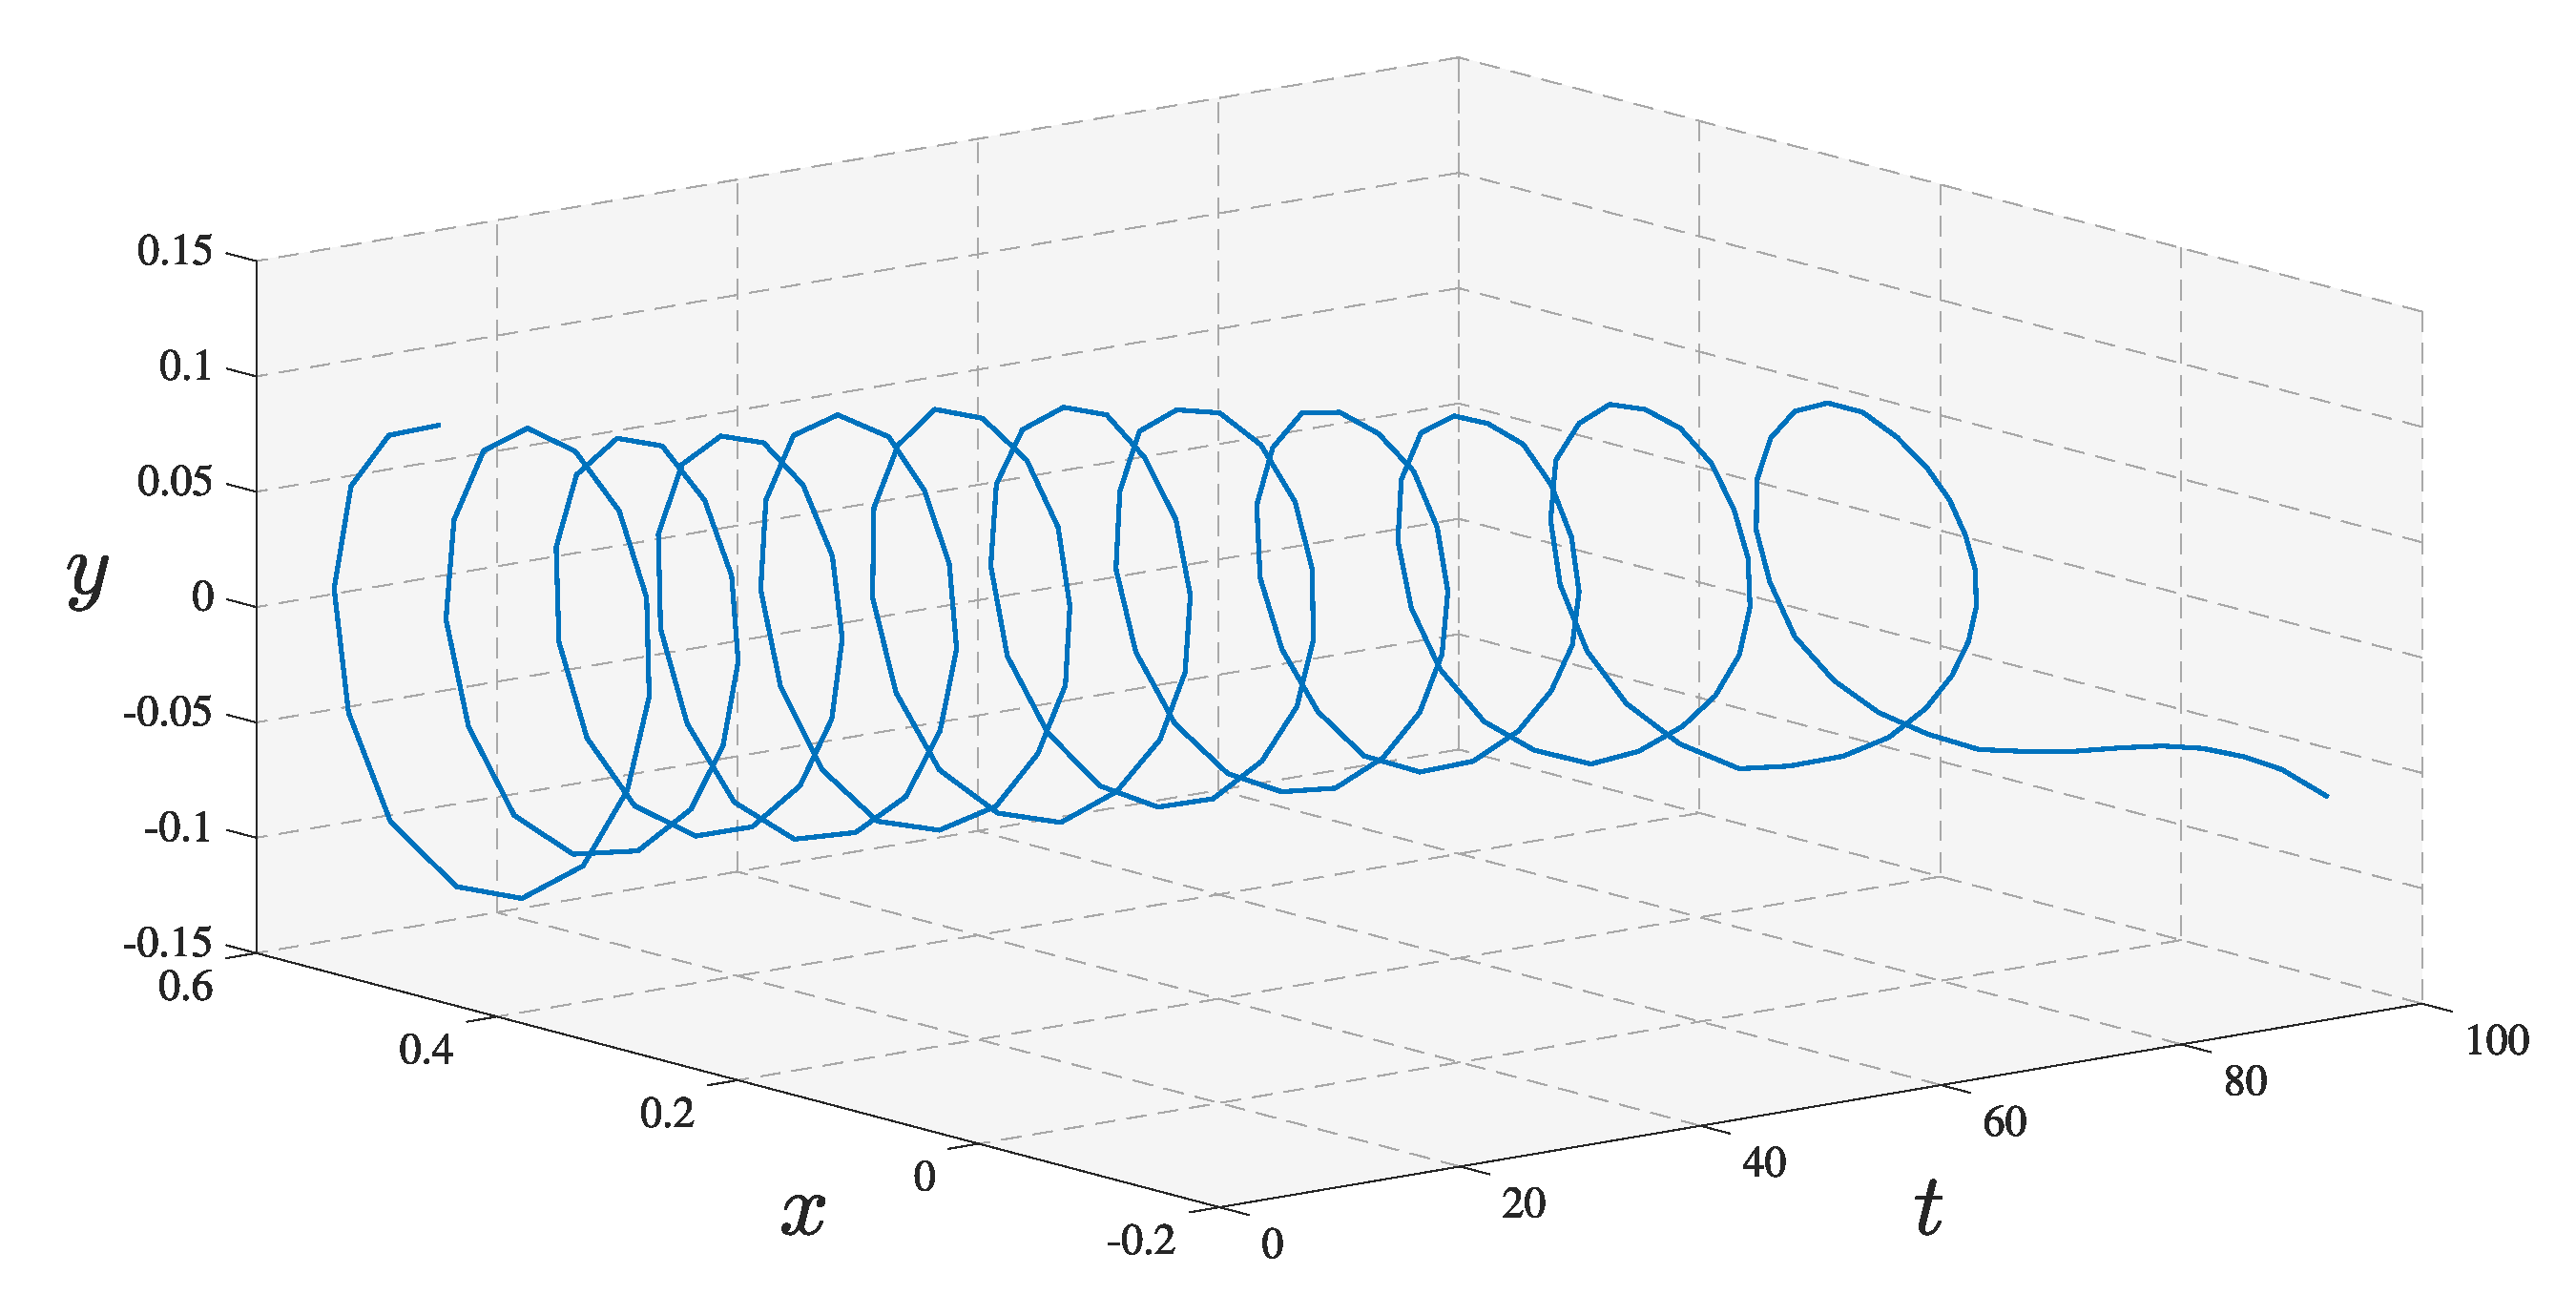
\includegraphics[width = 0.9\columnwidth]{Homoclinic3D}
	\caption{A single realisation of the system in equation~\ref{eqn:2D:homoclinicSystem} with initial point $(\sqrt{0.2},0.1)$. The system spirals around the moving centre at $(\sqrt{\alpha},0)$, $\alpha$ is given in equation~\ref{eqn:2D:homoclinicAlpha}, until $t=100$, $\alpha=0$, when the bifurcation occurs and the system tends towards infinity in the negative $x$ and negative $y$ directions.
		\label{fig:2D:Homoclinic3D}}
\end{figure}

We consider the system given by equations
	\begin{equation}
		\begin{array}{rcl}
		\dot{x} &=& y + \eta^{(x)},\\
		\dot{y} &=& \alpha - x^2 + \eta^{(y)},
		\end{array}
	\label{eqn:2D:homoclinicSystem}
	\end{equation}
where $\eta^{(x)}$, $\eta^{(y)}$ are white noise terms. If we ignore these noise terms, we find that the system has steady state solutions at $(x,y) = (\pm \sqrt{\alpha},0)$. The Jacobian of the system is given by 
	\begin{equation}
		J(x,y) = \left(\begin{array}{cc}
		0 & 1 \\ -2x & 0
		\end{array}\right)\,,
	\label{eqn:2D:homoclinicJacobian}
	\end{equation}
and has eigenvalues $\lambda = \pm \sqrt{-2x}$. The eigenvalues at the stable solutions are:
\begin{itemize}
	\item at $(-\sqrt{\alpha},0)$: $\lambda = \pm(4\alpha)^{1/4}$, indicating that this is a saddle,
	\item at $(+\sqrt{\alpha},0)$: $\lambda = \pm i(4\alpha)^{1/4}$, indicating that this is a stable centre.
\end{itemize}
\cite{williamson2015} allow $\alpha$ to vary and to approach zero from above. At $\alpha=0$ the two stable points collide resulting in a bifurcation and there are no stable solutions for $\alpha<0$. {\Red{ Before the bifurcation, the evolution of the system resembles a near-homoclinic orbit around the stable centre. This orbit becomes more and more pointed as the bifurcation approaches as the system spends more and more time close to the saddle point on each period. This looks like a system approaching a homoclinic bifurcation, in which the orbit eventually joins with the saddle and becomes homoclinic, and then disconnects from the saddle with further change in the system parameter (see equation~\ref{eqn:intro:trueHomoclinic}, page~\pageref{eqn:intro:trueHomoclinic} for an example of such a system). In this system, however, the orbit shrinks around the stable centre and, at the point of bifurcation, the centre meets with the saddle at the same time at which the orbit shrinks down to zero-radius, so the orbit does not actually become homoclinic. 
		
If we consider the system equations without the stochastic component, that is,
	\begin{equation}
	\begin{array}{rcl}
		\dot{x} &=& y ,\\
		\dot{y} &=& \alpha - x^2 ,
		\end{array}
		\label{eqn:2D:homoclinicSystem_deterministic}
	\end{equation}
we note this is equivalent to the second order differential equation
	\begin{equation}
		\ddot{x} = \alpha - x^2,
	\label{eqn:2D:homoclinicSystem_secondorder}
	\end{equation}
which has potential function
	\begin{equation}
		V(x) = \frac{x^3}{3} - \alpha x,
	\end{equation} 
since this results in
	\begin{equation}
		\ddot{x} = -\frac{\partial}{\partial x}V(x)\,.
	\end{equation} 
Since the energy 
	\begin{equation}
		E(x) = \frac{\dot{x}^2}{2}+V(x) = \frac{y^2}{2} + \frac{x^3}{3} - \alpha x\,,
	\end{equation} 
is a conserved quantity, that is, $\dot{E}(x)=0$, $E(x)=c$ for some constant $c$, then we have that the solutions to the ODE are given by
	\begin{equation}
		\frac{y^2}{2} + \frac{x^3}{3} - \alpha x =c\,.
		\label{eqn:2D:SystemA_solutions}
	\end{equation} 
This set of solutions is represented in figure~\ref{fig:2D:systemA_circles} where the solution is plotted for $10$ values of $c$ in the range $-1\leq c \leq 1$, with $\alpha=1$. We note the stable point at $x=\sqrt{\alpha}=1,~ y=0$ surrounded by concentric egg-shape `circles'. Thus, the system is not spiralling inwards toward the stable point, nor outwards. 
	}}

\begin{figure}
	\centering
	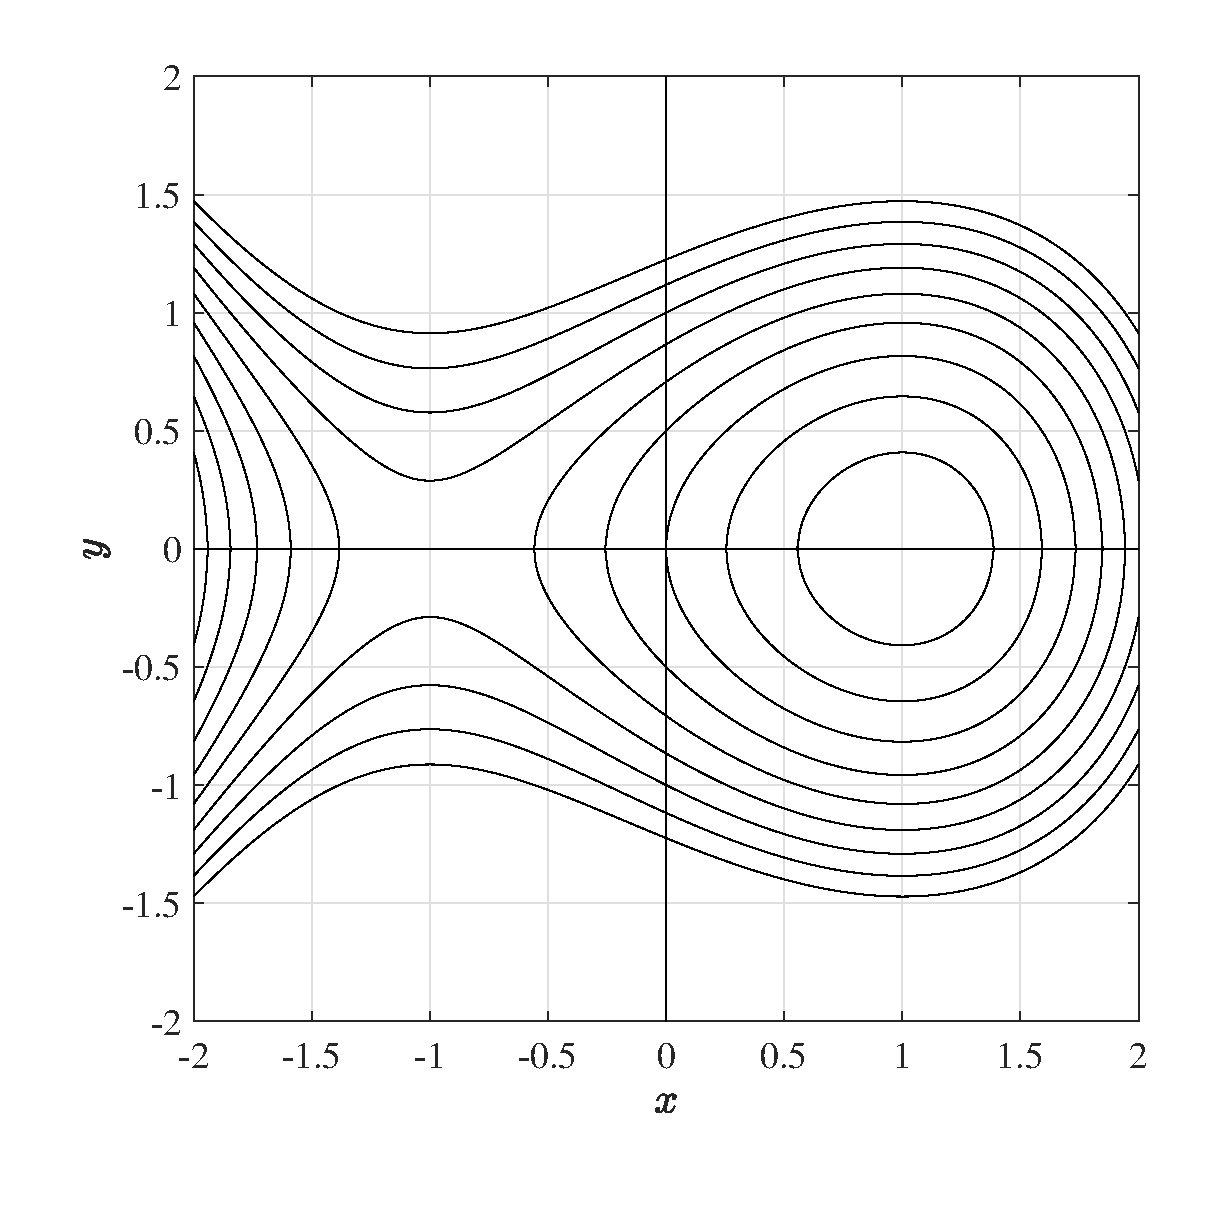
\includegraphics[width = 0.4\columnwidth]{systemA_circles}
	\caption{\Red{The solutions for System A (see equation~\ref{eqn:2D:SystemA_solutions}) are plotted for $\alpha=1$ with $10$ values of $c$ in the range $-1\leq c \leq 1$. A single stable point occurs at $(1,0)$ while a saddle exists at $(\m1, 0)$.
	}}
	\label{fig:2D:systemA_circles}
\end{figure}
%systemA_circles


\cite{williamson2015} consider a point at or close to the stable centre 
$(+\sqrt{\alpha},0)$, with noise terms $\eta^{(x)}$, $\eta^{(y)}$ in equation \ref{eqn:2D:homoclinicSystem} having standard deviation of 0.01. At this centre the eigenvalues of the Jacobian have zero real part but imaginary part of $\pm(4\alpha)^{1/4}$. If we take the eigenvalue with positive imaginary part we expect to see it decrease as $\alpha$ decreases to zero. This is the early warning signal of the bifurcation. 

We integrate the system in equations \ref{eqn:2D:homoclinicSystem} from $t=0$ to $t=100$, using a varying parameter
	\begin{equation}
		\alpha(t) = 0.2 - 0.002t,
	\label{eqn:2D:homoclinicAlpha}
	\end{equation}
so that the bifurcation when $\alpha = 0$ will occur at $t=100$. Noise terms $\eta^{(x)}$, $\eta^{(y)}$ are independent with zero mean and standard deviation 0.01 and the solution is sampled at intervals of $\Delta t = 0.5$. The result of one such integration is plotted in figure~\ref{fig:2D:Homoclinic3D}.

\begin{figure}
	\centering
	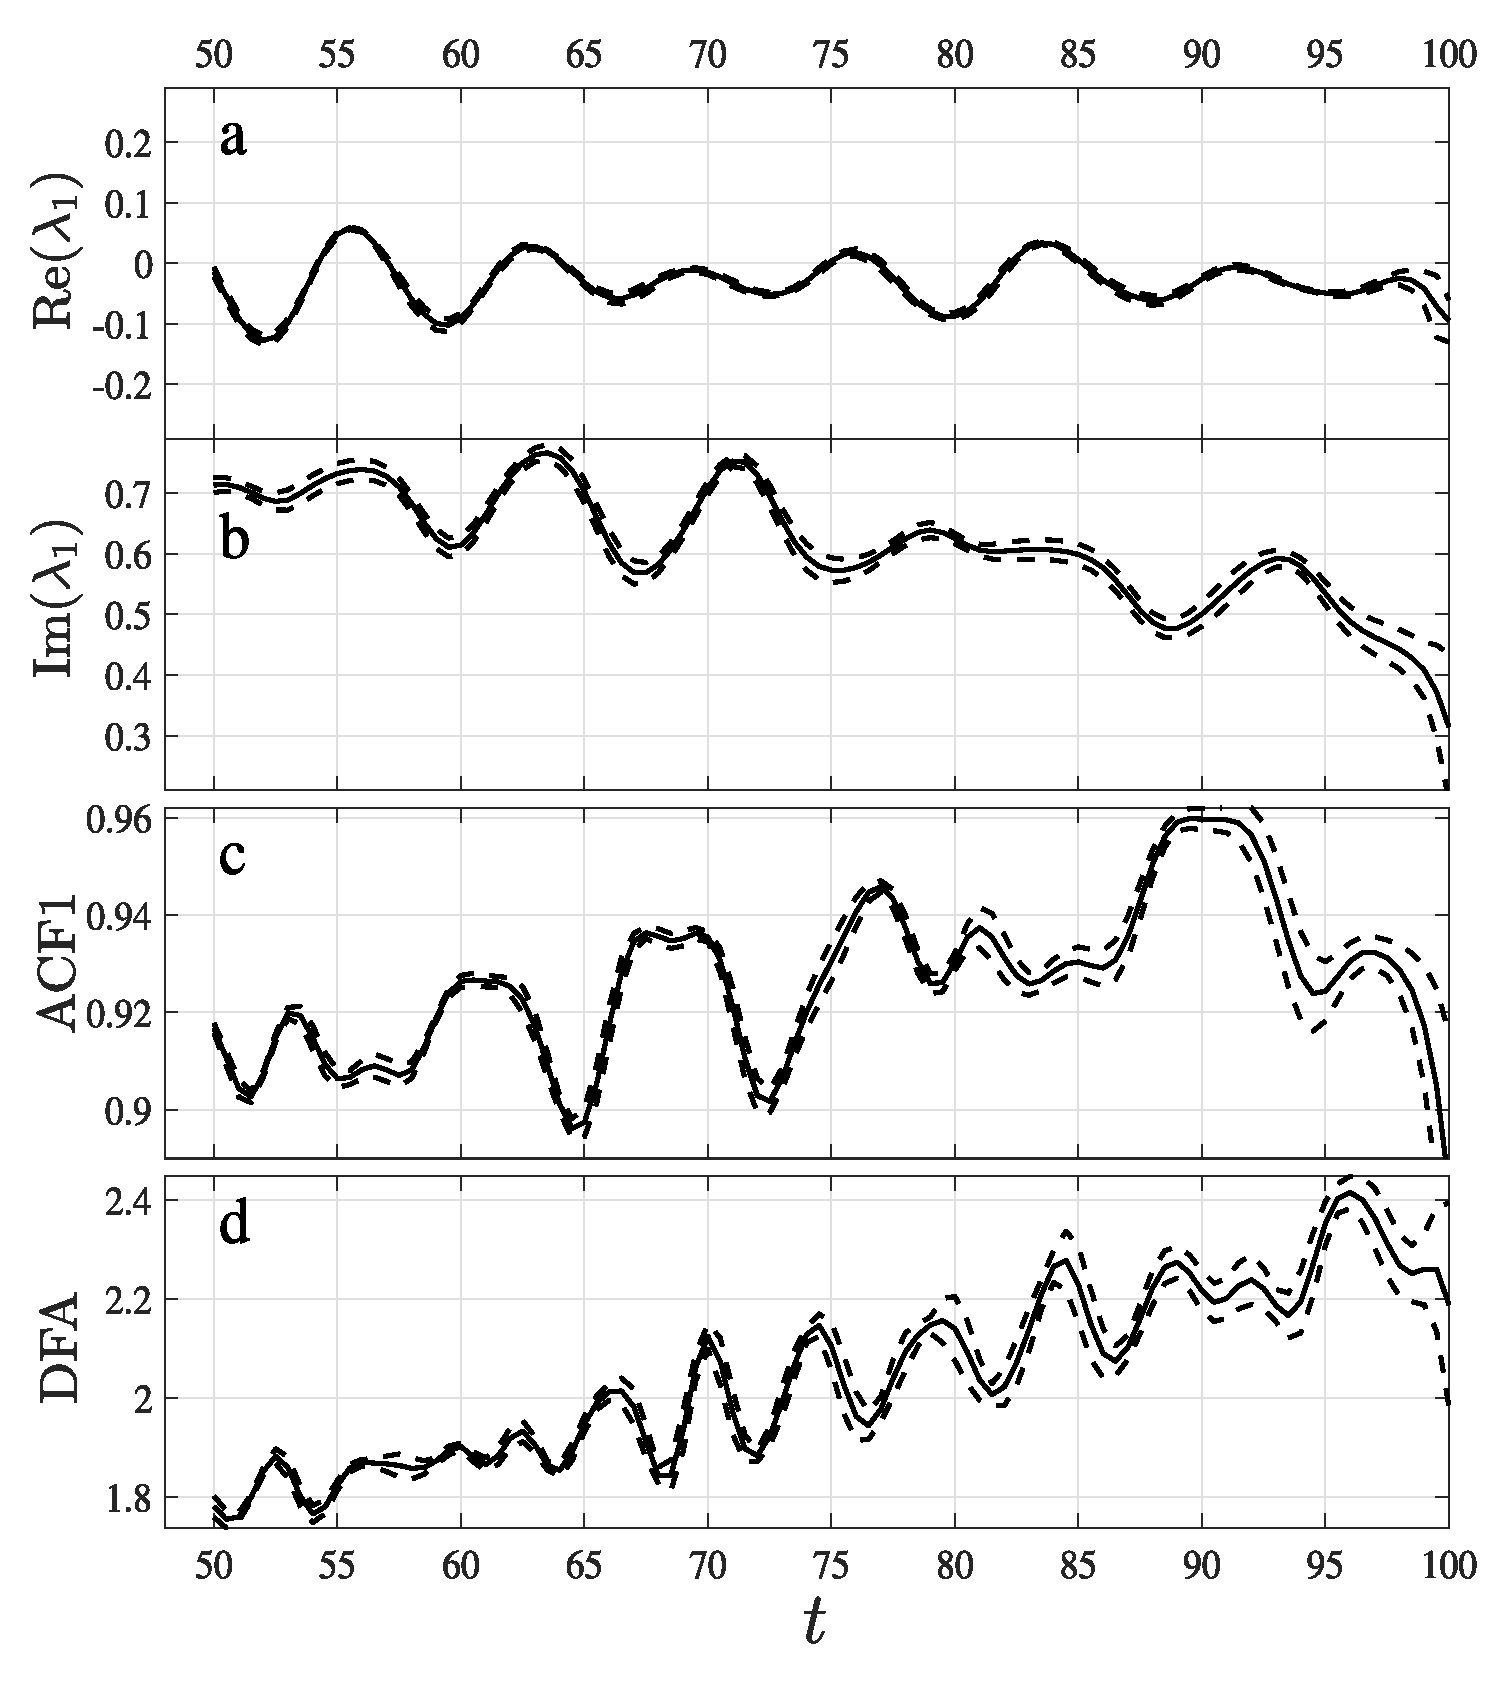
\includegraphics[width = 0.9\columnwidth]{HomoclinicIndicators}
	\caption{Tipping point indicators applied to System A (equation~\ref{eqn:2D:homoclinicSystem}) which experiences a bifurcation at $t=100$. Panels \textbf{a} and \textbf{b} show the real and imaginary parts of the first reconstructed eigenvalue of the Jacobian matrix, as in equation~\ref{eqn:2D:williamson-eigenvalueRelations}. Panels \textbf{c} and \textbf{d} show the ACF1 and DFA indicators calculated with a window size of 100 points, applied to the one-dimensional time series obtained by applying EOF dimension reduction to the data. The system was integrated ten times and the mean over ten data sets is plotted, along with error of one standard deviation (dashed lines).
	\label{fig:2D:HomoclinicIndicators}}
\end{figure}

We now attempt to provide an early warning signal of the impending bifurcation. The autocorrelation matrix $A$ is calculated using equation \ref{eqn:2D:williamson-AR1analogue} in a sliding window of 100 points. The Jacobian eigenvalues are recovered using equations \ref{eqn:2D:williamson-eigenvalueRelations} and the real and imaginary parts of the first eigenvalue (the eigenvalue with positive imaginary part) are calculated. This procedure is applied to ten realisations of the system, and the mean is shown in figure~\ref{fig:2D:HomoclinicIndicators}a,b with error bars of one standard deviation. The figure shows a successful reproduction of the results of \citet{williamson2015}: the real part of the eigenvalue is $\approx 0$ with little variability, as expected for $\mu>0$, and the decreasing imaginary part of the eigenvalue predicates the bifurcation as $\alpha\rightarrow0$, as predicted by the analysis. 

As a comparison, the ACF1 and DFA indicators are applied to the same data using a 100 point window size and after reducing the dimension of the system using EOFs. The results are shown in figure~\ref{fig:2D:HomoclinicIndicators}c,d. Both indicators show a general upwards trend prior to the bifurcation at $t=100$, but the ACF1 indicator contains more variability. 



\subsubsection{System experiencing a Hopf bifurcation (System B)}
\label{subsec:2D:MethodsApplied:WilliamsonHopf}

\begin{figure}
	\centering
	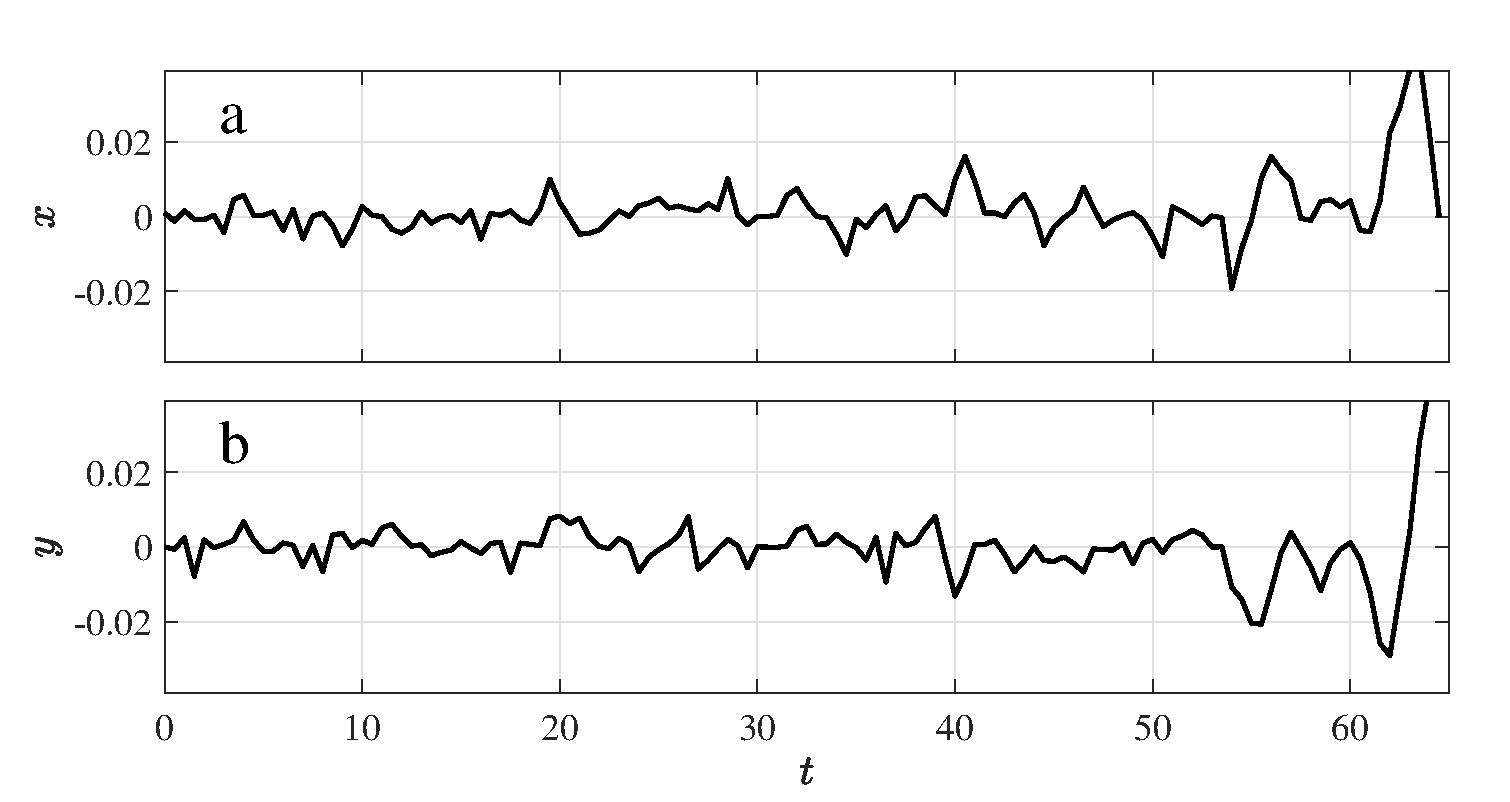
\includegraphics[width = 0.9\columnwidth]{HopfIllustration_EM}
	\caption{A single realisation of the system in equation~\ref{eqn:2D:HopfSystem_noise} with initial point $(0,0)$. The system oscillates about the stable point $(0,0)$ until $t=58$ when the bifurcation occurs and the stability is lost.
		\label{fig:2D:HopfIllustration}}
\end{figure}

We now consider the second example given by \citet{williamson2015}, the system given by the polar equations 
	\begin{equation}
		\begin{array}{rcl}
			\dot{r} &=& \mu r - r^3,\\
			\dot{\theta} &=& 1 + r^2.
		\end{array}
		\label{eqn:2D:HopfSystem}
	\end{equation}
The system is a classic example of a supercritical Hopf bifurcation. The normal form of the Hopf bifurcation is
\begin{equation}
	\dot{z} = z\left((\lambda+i)+b|z|^2\right),
\end{equation}
where $z$ and $b=\alpha+i\beta$ are complex numbers. 
If we rewrite the system in equation \ref{eqn:2D:HopfSystem} according to $z = \exp(i\theta)$, we get
	\begin{align}
		\begin{split}
			\dot{z} &= \dot{r}e^{i\theta}+ir\dot{\theta}e^{i\theta}\\
			&= re^{i\theta}\left(\frac{\dot{r}}{r}+i\dot{\theta}\right)\\
			&= re^{i\theta}\left((\mu-r^2)+i(1+r^2)\right)\\
			&= z\left((\mu+i)+(i-1)|z|^2\right).
		\end{split}
	\end{align}

The system has stable solution at $r=0$ for $\mu<0$. At $\mu=0$ a bifurcation occurs and $r=0$ becomes unstable, whilst two stable solutions for $r$ are created at $r = \pm\sqrt{\mu}$. Since $\theta$ increases at a constant rate $\dot{\theta}=1+\mu$, or almost constant if an additional noise term is introduced into equation~\ref{eqn:2D:HopfSystem}, this results in a stable limit cycle with radius $r=\sqrt{\mu}$. 

We may also investigate the nature of the bifurcation by studying the eigenvalues of the Jacobian of the system equations. In Cartesian rather than polar coordinates we have
	\begin{equation}
		J(x,y) =  
		\left(
		\begin{array}{cc}
		\mu - (x+y)^2-2x^2 & -1-(x+y)^2-2y^2\\
		1+(x-y)^2 + 2x^2 & \mu - (x-y)^2-2y^2
		\end{array} \right).
	\label{eqn:2D:HopfJacobian}
	\end{equation}
At the stable point $r=0$ (i.e. $(x,y)=(0,0)$), the matrix $J(x,y)$ has complex conjugate eigenvalues $\lambda=\mu\pm i$. The system therefore experiences a Hopf bifurcation as $\mu$ approaches zero from below, characterised by the Jacobian eigenvalues moving from the negative-real to the positive-real half of the complex plane.

We reproduce the numerical results of \citet{williamson2015} using a varying parameter
	\begin{equation}
		\mu(t) = 0.05t - 2.9\,,
	\label{eqn:2D:HopfParameter}
	\end{equation} 
and integrate the system from $t=0$ to $t=60$ with the solution given at intervals $\Delta t = 0.2$. The bifurcation at $\mu = 0$ will occur at $t=58$. Gaussian noise terms $\eta^{(r)}$ and $\eta^{(\theta)}$ are also added to the system equations for $r$ and $\theta$ respectively:
	\begin{equation}
		\begin{array}{rcl}
		\dot{r} &=& \mu r - r^3 + \eta_r\,,\\
		\dot{\theta} &=& 1 + r^2 + \eta_\theta\,,
		\end{array}
	\label{eqn:2D:HopfSystem_noise}
	\end{equation}
where $\eta_r$, $\eta_\theta$ both have zero mean and standard deviation $0.01$. The result is shown in figure~\ref{fig:2D:HopfIllustration}. 

\begin{figure}
	\centering
	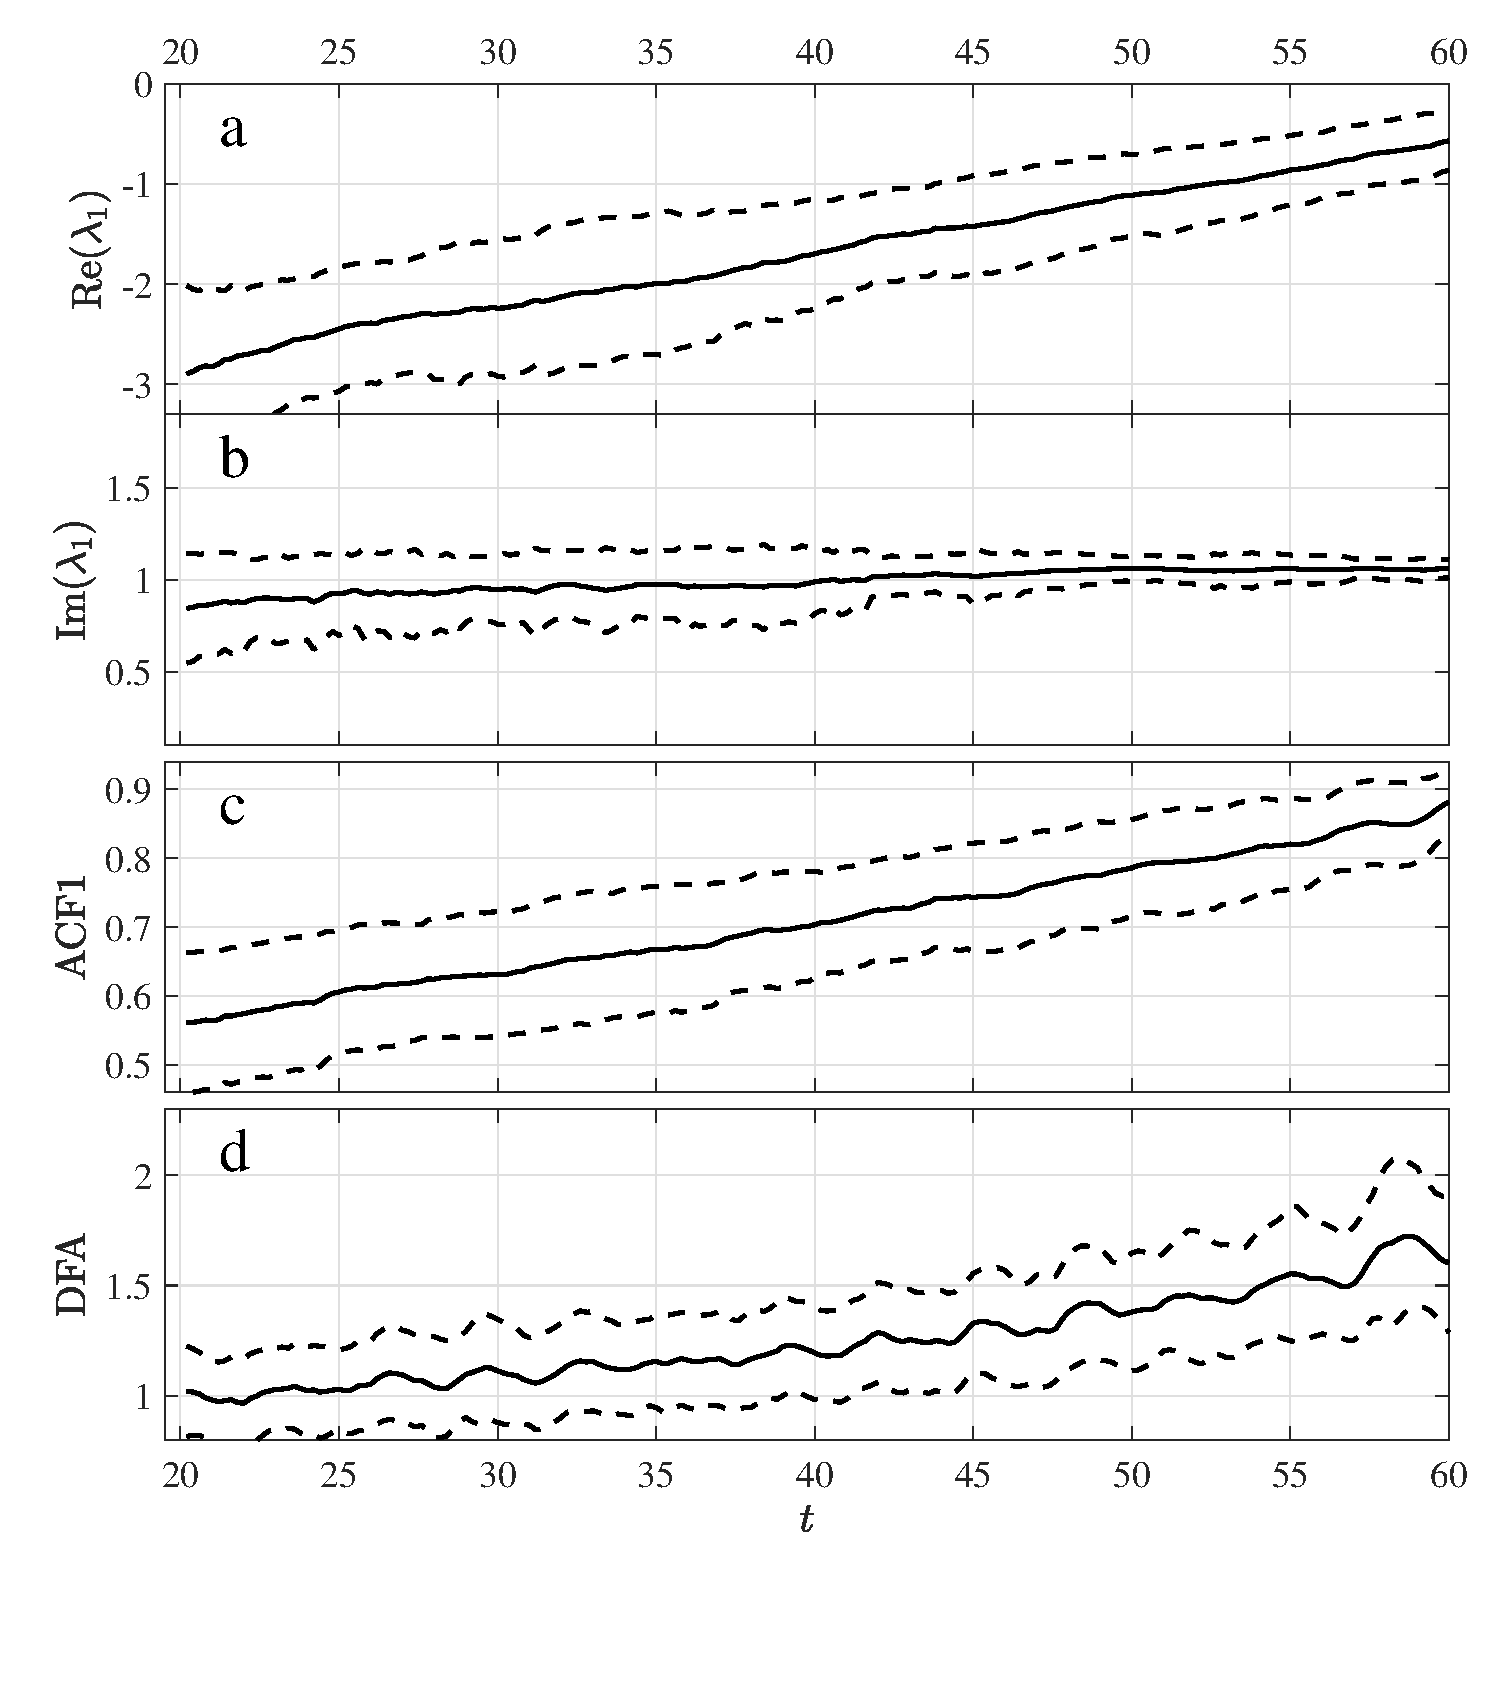
\includegraphics[width = 0.9\columnwidth]{HopfIndicators_EM}
	\caption{Tipping point indicators applied to System B (equation~\ref{eqn:2D:HopfSystem_noise}) which experiences a Hopf bifurcation at $t=58$. Panels \textbf{a} and \textbf{b} show the real and imaginary parts of the first reconstructed eigenvalue of the Jacobian matrix, as in equation~\ref{eqn:2D:williamson-eigenvalueRelations}. Panels \textbf{c} and \textbf{d} show the ACF1 and DFA indicators calculated with a window size of 100 points, applied to the one-dimensional time series obtained by applying EOF dimension reduction to the data. The system was integrated $100$ times and the mean over the $100$ data sets is plotted, along with error of one standard deviation (dashed lines).
		\label{fig:2D:HopfIndicators}}
\end{figure}

As in the previous example, the autocorrelation matrix $A$ is calculated using equation~\ref{eqn:2D:williamson-AR1analogue} in a sliding window of 100 points. The Jacobian eigenvalues are recovered using equation~\ref{eqn:2D:williamson-eigenvalueRelations} and the real and imaginary parts of the first eigenvalue are plotted in figure~\ref{fig:2D:HopfIndicators}a,b.

In this example, as in the previous, we are able to successfully reproduce the results of \citet{williamson2015}.


\subsubsection{The Van der Pol oscillator (System C)}
\label{subsec:2D:MethodsApplied:WilliamsonVanDerPol}
\begin{figure}
	\centering
	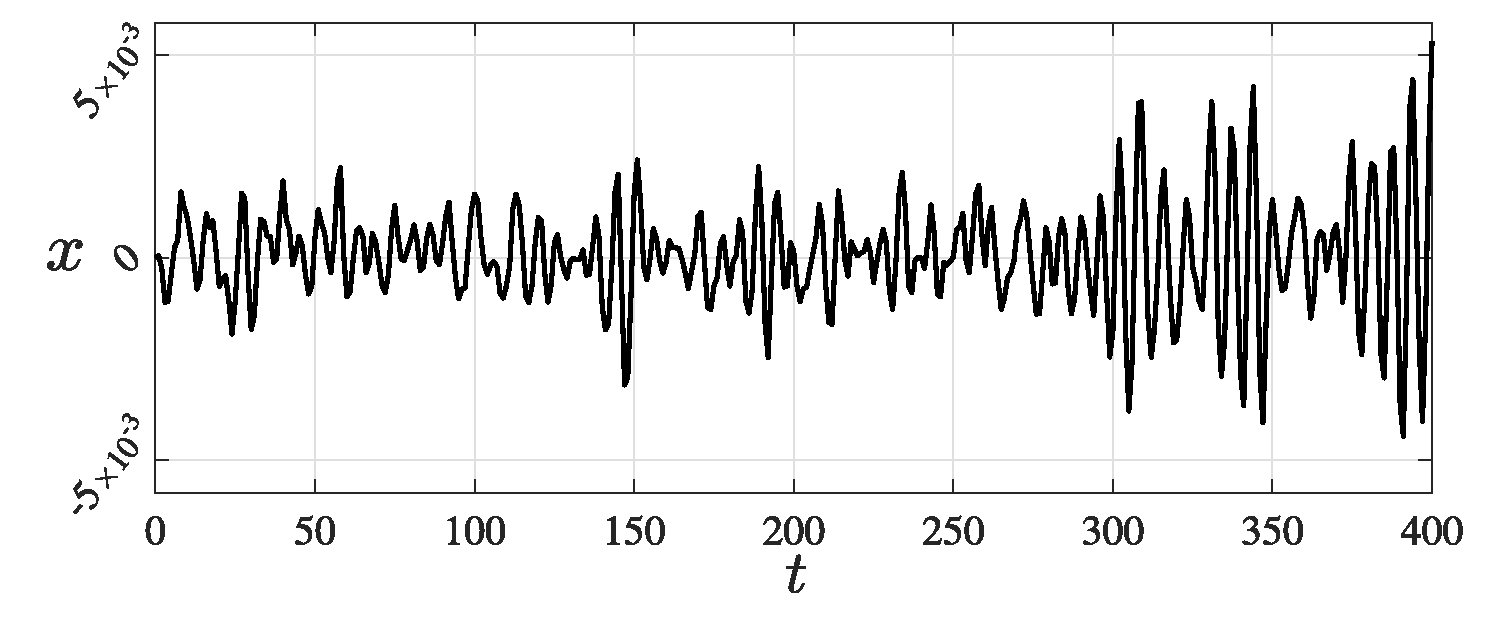
\includegraphics[width = 0.9\columnwidth]{vdpIllustration}
	\caption{A single realisation of the Van der Pol system in equation~\ref{eqn:2D:VDPSystemCoupled} with initial point $(0,0)$. The system oscillates about the centre at $(0,0)$ until $t=380$, $\mu=0$, when the Hopf bifurcation occurs and stability is lost.
		\label{fig:2D:vdpIllustration}}
\end{figure}

Here, we consider another example of a Hopf bifurcation, allowing us to apply the method introduced by \citet{williamson2015} to a novel system. We consider the Van der Pol oscillator \citep{vanDerPol1926} given by
	\begin{equation}
		\ddot{x} - \mu(1-x^2)\dot{x} + x = \eta,
		\label{eqn:2D:VDPSystem}
	\end{equation}
where the stochastic forcing term $\eta$ is white noise with standard deviation 0.01. We may also write equation \ref{eqn:2D:VDPSystem} as a coupled system of first order ODEs:
	\begin{equation}
		\begin{array}{rcl}
		\dot{x} &=& \mu\left(x - \frac{1}{3}x^3\right)+y,\\
		\dot{y} &=& -x + \eta.
		\end{array}
		\label{eqn:2D:VDPSystemCoupled}
	\end{equation}
The system has a stable equilibrium point ($\dot{x}= \dot{y}= 0$) at $(x,y)= (0,0)$ for $\mu<0$ which becomes the centre of a stable limit cycle for $\mu>0$. The Jacobian of this system is calculated:
	\begin{equation}
		J(x,y) = \left(
		\begin{array}{cc}
		\mu(1-x^2) & 1\\
		-1 & 0
		\end{array}
		\right).
		\label{eqn:2D:VDPJacobian}
	\end{equation}
Evaluated at the stable point $(0,0)$, the two complex-conjugate eigenvalues of the Jacobian are $\lambda = \frac{1}{2}(\mu \pm \sqrt{\mu^2-4})$. We therefore expect that the real part of both of the eigenvalues, equal to $\mu/2$, will approach zero as $\mu$ approaches zero from below, i.e. as the system approaches the bifurcation. 

We integrate the system in equations \ref{eqn:2D:VDPSystemCoupled} from $t=0$ to $t=400$ using a time dependent parameter
	\begin{equation}
		\mu(t) = -0.38 + 0.001t,
		\label{eqn:2D:vdpParameter}
	\end{equation} 
so that the bifurcation $\mu=0$ will occur at $t=380$. Using the method described, we estimate the first eigenvalue of the Jacobian in a sliding window of 100 points. The mean (with error bars of one standard deviation) of 10 such experiments is shown in figure~\ref{fig:2D:vdpIndicators}. We note that the real part of the eigenvalue increases as expected and provides an early warning signal of the impending Hopf bifurcation.

\begin{figure}
	\centering
	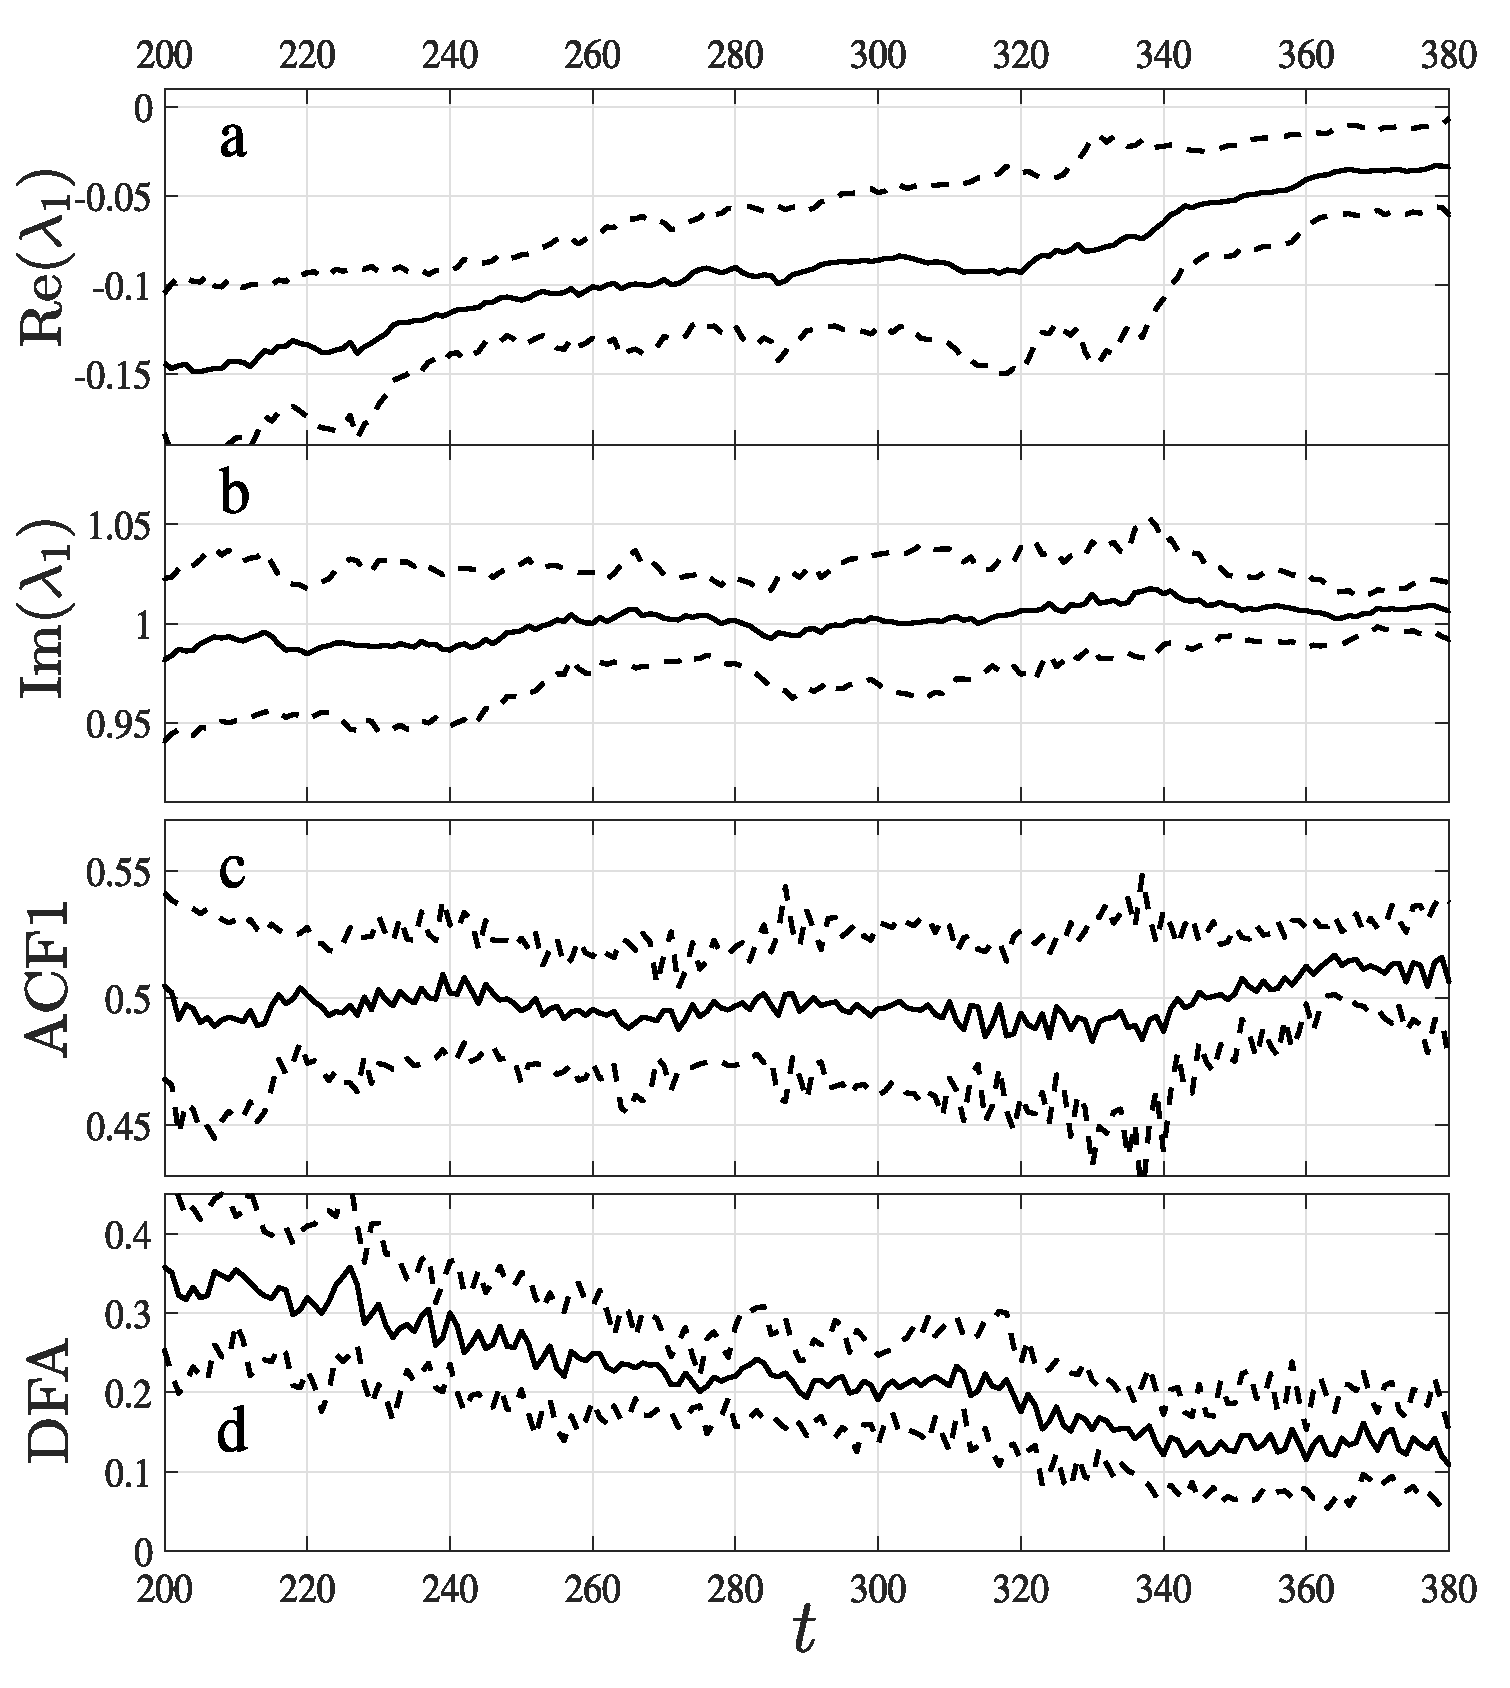
\includegraphics[width = 0.9\columnwidth]{VdpIndicators}
	\caption{Tipping point indicators applied to System C, the Van de Pol oscillator (equation~\ref{eqn:2D:VDPSystemCoupled}), which experiences a Hopf bifurcation at $t=380$. Panels \textbf{a} and \textbf{b} show the real and imaginary parts of the first reconstructed eigenvalue of the Jacobian matrix, as in equation~\ref{eqn:2D:williamson-eigenvalueRelations}. Panels \textbf{c} and \textbf{d} show the ACF1 and DFA indicators calculated with a window size of 100 points, applied to the one-dimensional time series obtained by applying EOF dimension reduction to the data. The system was integrated ten times and the mean over ten data sets is plotted, along with error of one standard deviation (dashed lines).
		\label{fig:2D:vdpIndicators}}
\end{figure}

\subsection{Application of the novel PS indicator}
\label{subsec:2D:MethodsApplied:PS-indicator}

We also calculate the PS indicator in the three systems described in this section, in addition to the ACF1 and DFA indicators and the Jacobian eigenvalues as shown in figures~\ref{fig:2D:HomoclinicIndicators}-\ref{fig:2D:vdpIndicators}. Systems A, B and C (see equations~\ref{eqn:2D:homoclinicSystem}, \ref{eqn:2D:HopfSystem_noise} and \ref{eqn:2D:VDPSystemCoupled}) are integrated and the PS indicator is calculated, in all three cases, using a sliding window of 100 points, similarly to the other indicator methods. This is done ten times for each system and the mean of the PS indicator is found, as shown in figure~\ref{fig:2D:PS-indicators}. We see that the PS indicator does not provide an EWS for the bifurcation in systems A and C, and the signal is very weak, obscured by its variability, in system B. In all three cases the DFA indicator, as presented in figures~\ref{fig:2D:HomoclinicIndicators}-\ref{fig:2D:vdpIndicators}, provides a clearer EWS. 

\begin{figure}
	\centering
	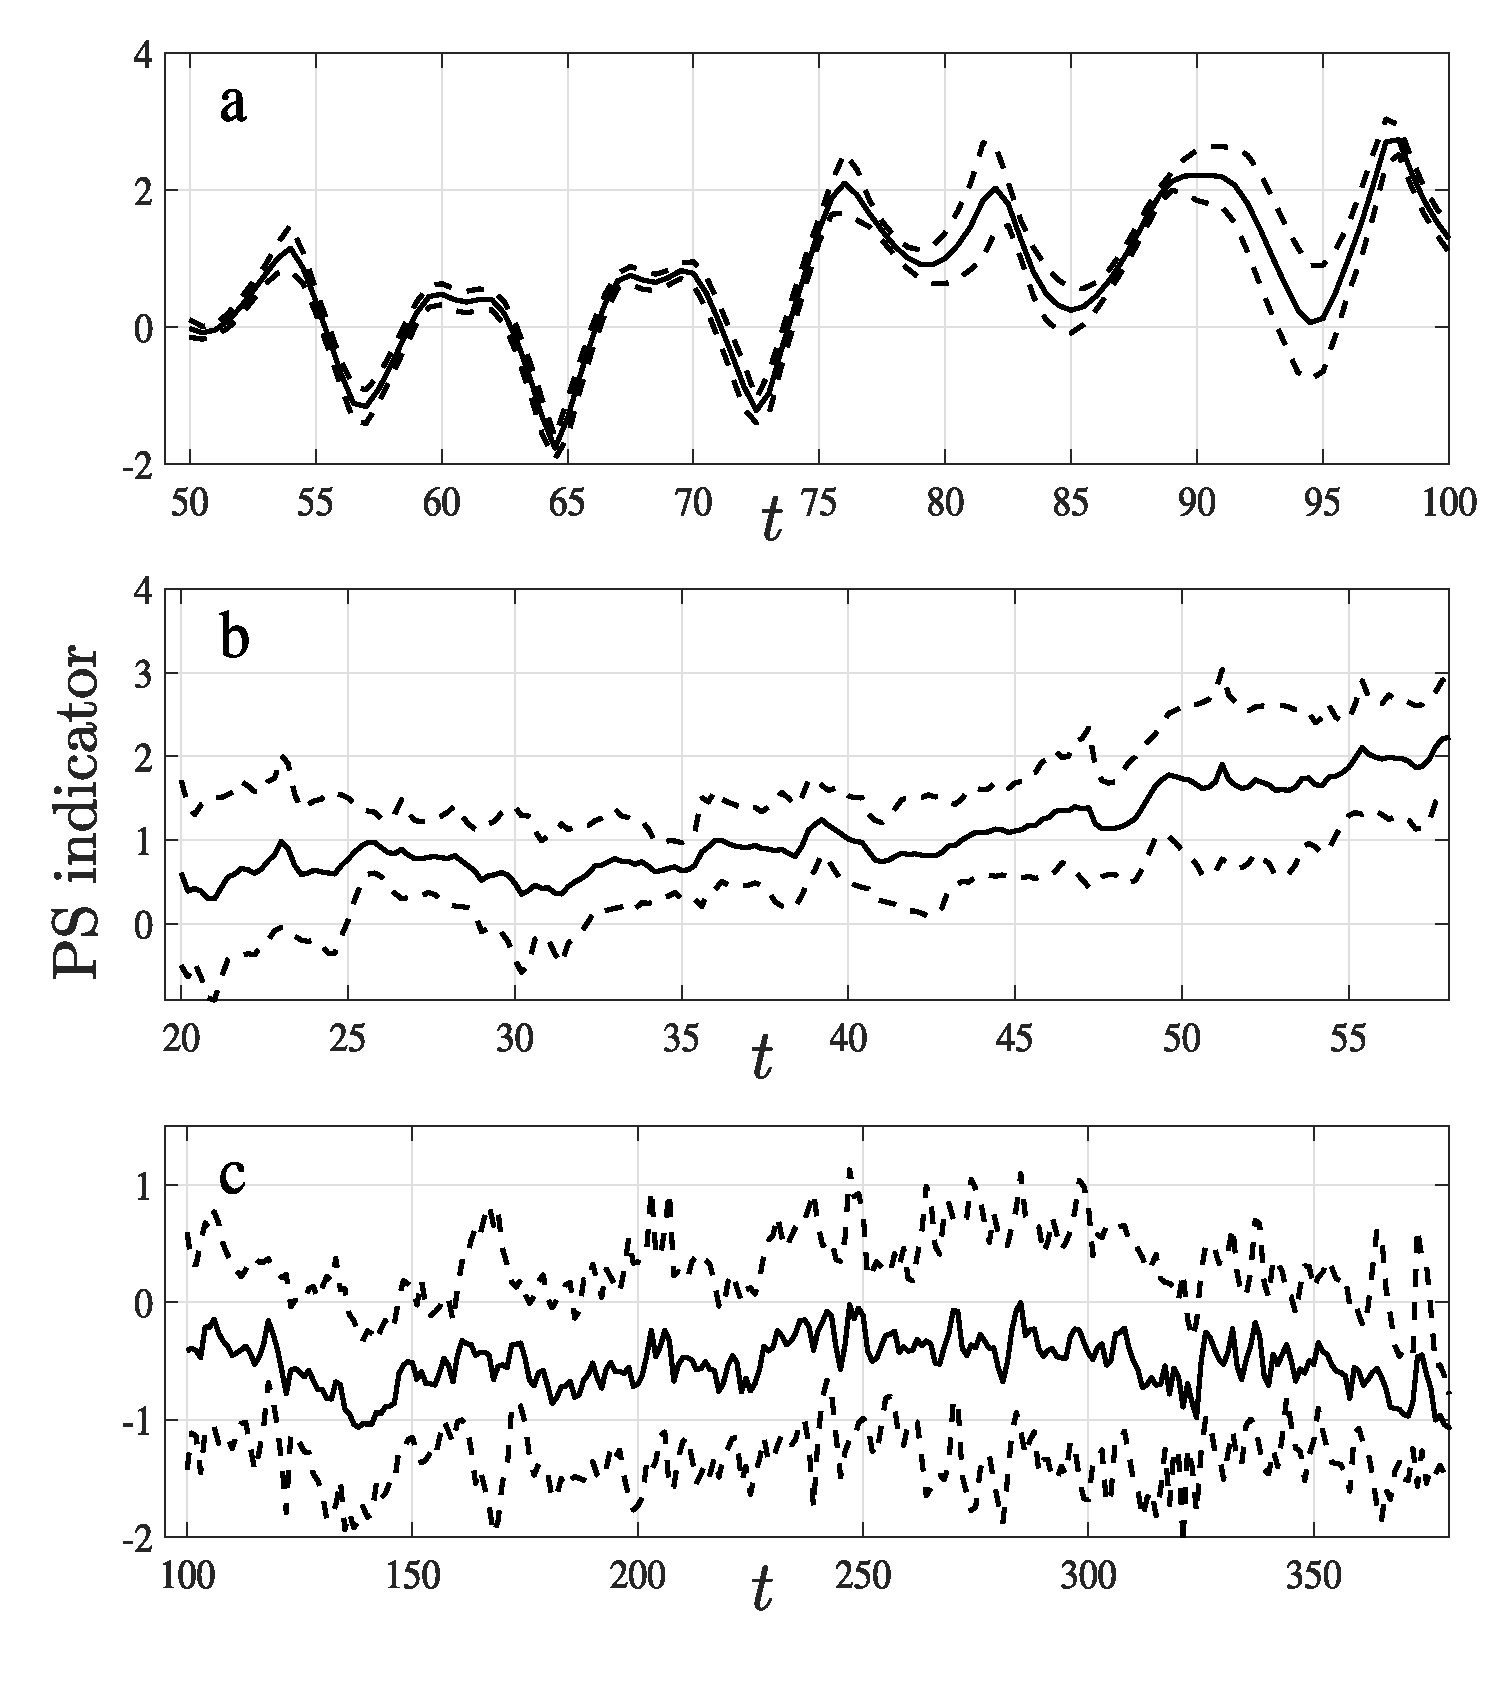
\includegraphics[width = 0.9\columnwidth]{PSindicators}
	\caption{PS indicator applied to the three systems described in this section after reducing each system to one dimension using the EOF method. The results for systems A, B and C are shown in panels \textbf{a}, \textbf{b} and \textbf{c} respectively. In each plot the bifurcation occurs at the last point on the $t$-axis: $t=100$, $t=58$ and $t=380$ respectively. Each system was integrated ten times and the mean over ten data sets is plotted, along with error of one standard deviation (dashed lines).
		\label{fig:2D:PS-indicators}}
\end{figure}



\subsection[Investigation of updated EOF projection]{Investigation of updated EOF projection with the ACF1 indicator}
\label{subsec:2D:MethodsApplied:Hopf_movingEOF}

In section~\ref{subsec:2D:EOF:movingEOF} it is remarked that in a practical prediction problem one cannot obtain a single EOF score with which to calculate a tipping point indicator. More sensibly, the EOF eigenvector, onto which the multi-variable time series is projected, would be updated at each iteration of the indicator calculation. Here we once again apply the ACF1 indicator to system B (see figure~\ref{fig:2D:HopfIndicators}b) but present the other available options. Figure~\ref{fig:2D:Hopf_movingEOF} shows the result of using the global EOF projection (as in figure~\ref{fig:2D:HopfIndicators}b) alongside the windowed EOF projection, in which only the current window of data is considered, and the moving EOF projection, in which the EOF eigenvector is updated using new data as time progresses without disregarding any previous data.
\begin{figure}
	\centering
	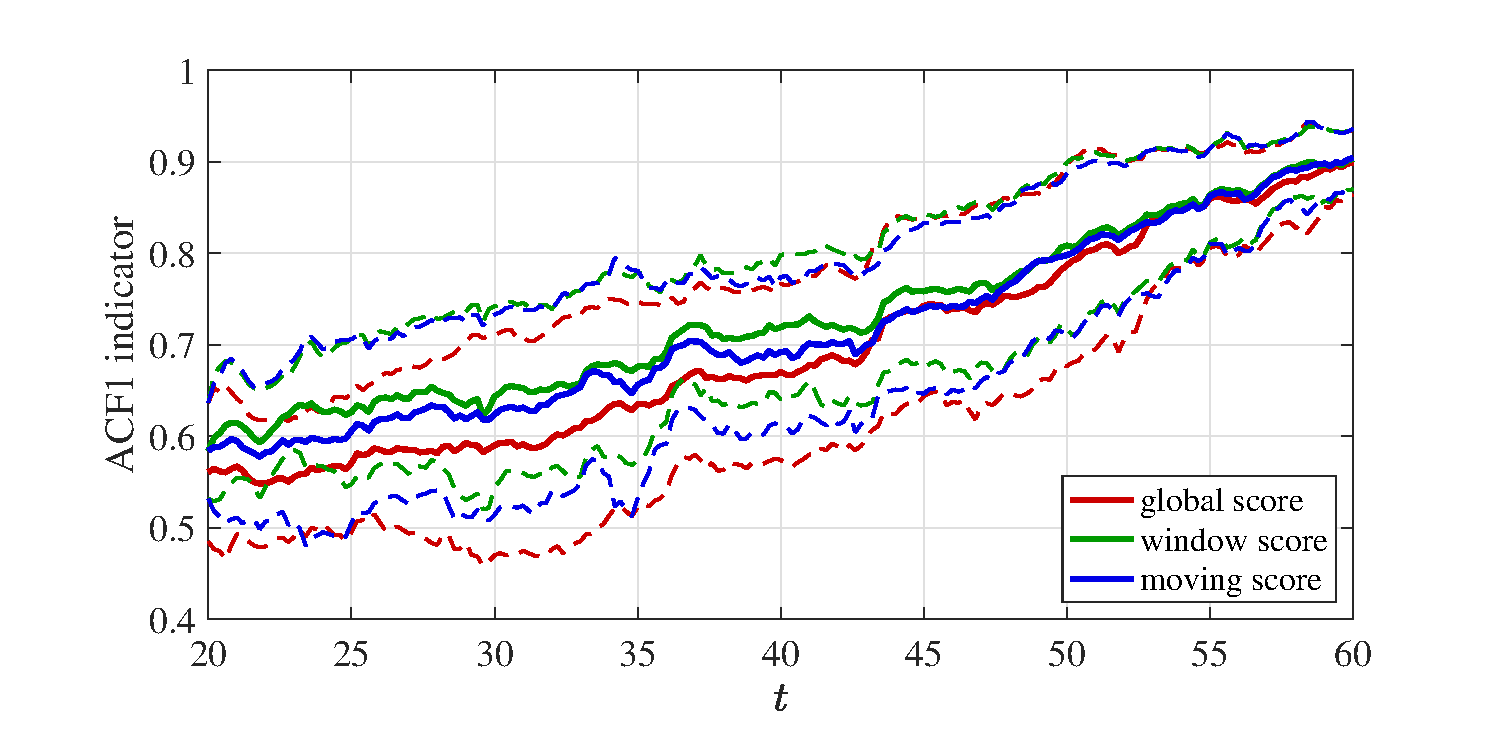
\includegraphics[width = 0.9\columnwidth]{HopfEOF}
	\caption{ACF1 indicator applied to System B in conjunction with EOF dimension reduction. Three different options for the EOF calculation are used: the global, windowed and moving EOF projections (red, blue and green respectively). For each of the three options, the system was integrated ten times and the mean over ten data sets is plotted, along with error of one standard deviation (dashed lines).
		\label{fig:2D:Hopf_movingEOF}}
\end{figure}

We note that the three options do not differ significantly. In particular, the fact that the global and windowed approaches yield very similar results demonstrates that the principal EOF eigenvector does not change significantly over time. In systems where the EOF eigenvector is likely to change over time, it would be best to use the windowed projection approach for practical problems so that the optimal variance-maximising projection is always used. However, this may introduce noise-induced error, particularly when the window size is short. 

\subsection{Discussion of results}
\label{subsec:2D:MethodsApplied:discussion}
{\Red{
In this section we have calculated the ACF1, DFA and PS indicators for three different dynamical systems in order to provide an early warning signal. Unlike in chapter~\ref{chap:1D} (see section~\ref{sec:1D:indicatorComparison}) we did not have a one-dimensional time series to which these methods might be applied, the EOF projections of the two-dimensional time series were therefore used. In addition we have obtained an additional early warning signal, from the `eigenvalue indicator', using the method of \cite{williamson2015} (see section~\ref{sec:2D:Williamson}). 

In the cases of Systems A and B the results of \cite{williamson2015} are faithfully reproduced. The imaginary part of the first eigenvalue decreases as an EWS of the bifurcation in System A, and the real part of the first eigenvalue increases as an EWS of the Hopf bifurcation in System B. When applied to System C, the Van der Pol oscillator, the real part of the first eigenvalue increases, which is to be expected since the tipping point in this case is also a Hopf bifurcation. We therefore verify the method in a new system, where the same indicator predicts the same variety of bifurcation (Hopf). 

The one-dimensional EWS methods introduced in chapter~\ref{chap:1D} were applied to the EOF projection of the time series in each case. We find that for Systems A and B these methods do provide an EWS in the sense that the indicators increase prior to the tipping point. That is, the indicators are higher in each case when the system parameter is closer to the critical value. This increase is clearer in the ACF1 and DFA indicators than in the PS indicator, and we note that the PS indicator also showed the least significant increase in all the one-dimensional systems studied in chapter~\ref{chap:1D}, so this is not surprising. In the case of System A, all three indicators suffer from large fluctuations which disguise any increase due to the presence of the tipping point itself. These fluctuations are likely due to the oscillations in System A, which orbits around the stable centre until it crosses the saddle node and diverges. This oscillation will be investigated further, and solutions proposed, in section~\ref{sec:2D:periodic_orbit}. 

In the case of System C, the Van der Pol oscillator, none of these three indicators provided an EWS. The ACF1 and PS indicators remained approximately constant as the bifurcation approached, whilst the DFA indicator apparently \emph{decreased} significantly. In this case the eigenvalue indicator performed much better than the combination of the EOF projection and the one-dimensional indicators. The problem may lie, again, with the oscillations in the system. 

}}


\section{Dealing with periodicity in an orbiting system}
\label{sec:2D:periodic_orbit}
{\Red{

The poor performance of the early warning indicators, and the DFA indicator in particular, when applied to System A (equation~\ref{eqn:2D:homoclinicSystem}), may be in part attributable to the periodicity in the system since the methods are not designed with this aspect in mind \citep{williamson2016}. The data may appear highly correlated even far from the bifurcation due to the fact that the system is following an orbit, although each orbit is in fact simply a noisy variation of the last. The DFA method removes trends only by subtracting a quadratic or cubic fit to the data and will not necessarily eliminate the correlation due to an orbit, particularly if more than one periods of the orbit occur within a single DFA window. 

In this section we investigate the effect of the presence of the orbit on the performance of the early warning indicators and attempt to improve performance by replacing the time series with its Poincaré map. As an example we again use System A:
\begin{equation}
	\begin{array}{rcl}
	\dot{x} &=& y + \eta^{(x)},\\
	\dot{y} &=& \alpha - x^2 + \eta^{(y)},
	\end{array}
	\label{eqn:2D:homoclinicSystem_again}
\end{equation}
(reprinting of equation~\ref{eqn:2D:homoclinicSystem}) where $\eta^{(x)}$ and $\eta^{(y)}$ are Gaussian white noise terms and $\alpha$ is a parameter affecting the nature of the stable states. For $\alpha>0$ the system has a stable centre at $(x,y) = (\sqrt{\alpha}, 0)$ and a saddle point at $(\m\sqrt{\alpha},0)$, at $\alpha=0$ the two points meet and there are no stable solutions for $\alpha<0$. If the system is initially close to the stable centre $(\sqrt{\alpha}, 0)$ it will orbit around this point, eventually either converging towards the centre or spiralling outwards until it leaves the orbit and diverges to infinity once it reaches the saddle node. Experimentally we find that for $\alpha=1$ the system diverges if the initial radius (with $(\sqrt{\alpha}, 0)$ as the centre) is greater than $\approx 0.24$. As $\alpha$ decreases toward zero this limiting radius also decreases so than an initially convergent system becomes divergent close to the bifurcation. 
}}
\begin{figure}
	\centering
	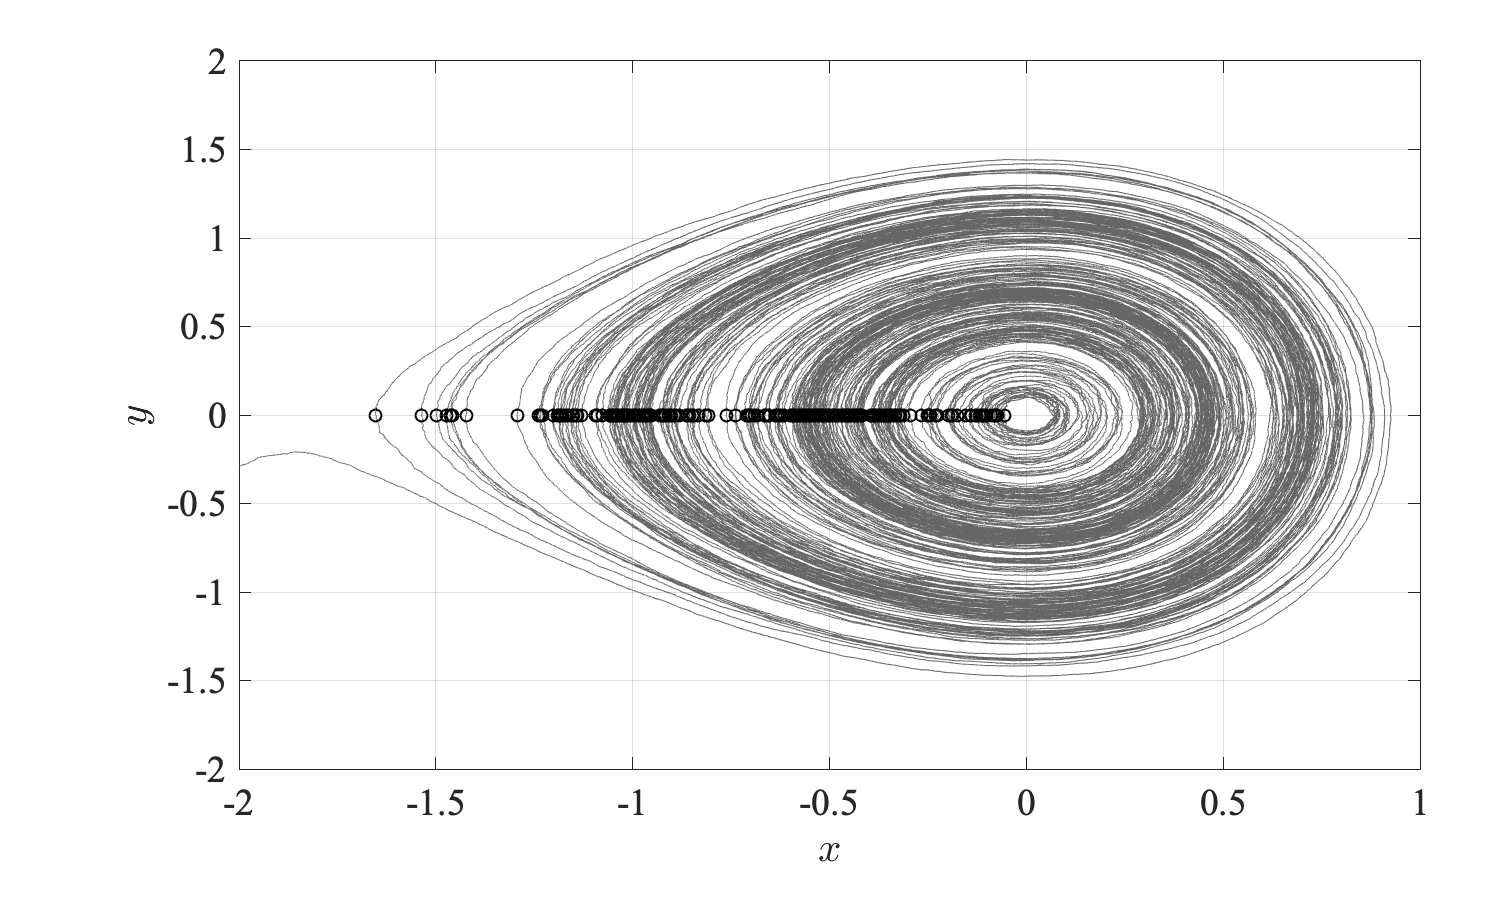
\includegraphics[width = 0.6\columnwidth]{periodicity_IntegrationPlusReturnPoints}
	\caption{\Red{ System A is integrated numerically with 
			$\Delta t = 0.01$ and $\alpha(t) = 1-10^{\m4}t$. The Poincar\'{e} return points for each orbit are also plotted (black circles).}}
	\label{fig:2D:periodicity:integration}
\end{figure}


\subsection{Methods}
\label{subsec:2D:periodic_orbit:methods}
{\Red{
In the original study of System A (see figure~\ref{fig:2D:HomoclinicIndicators}, page~\pageref{fig:2D:HomoclinicIndicators}) the periodicity was ignored and the early warning signals calculated using the raw data as an output of the numerical integration of the system equations. Here we present two alternative approaches to dealing with the periodicity.

\subsubsection{An approach based on the Poincaré map}

For a deterministic system $z(t)$ which orbits about a central point, the Poincaré map (see \cite{strogatz2014}) of a point $z(t_0)$ is the point $z(t_0+\tau) = P(z(t_0))$ such that the system has completed one periodic orbit during the time $\tau$. If $P(z(t_0)) = z(t_0)$ then the system has returned to exactly the same point after one period and therefore, if the system is deterministic, will continually repeat the same trajectory. 

In order to obtain a time series without oscillating behaviour, we consider the series of iterated Poincaré maps $z_n = P(z_{n-1})$ staring with an initial point $z_0$. In the case of System A (equation~\ref{eqn:2D:homoclinicSystem_again}) we take $z_0$ to be the first point on the half line $y=0,~x<\sqrt{\alpha}$, so that the series $[z_n]$ is the series of all the points which cross this half line as the system orbits around the point $(\sqrt{\alpha},0)$. We record only the $x$ coordinates since $y=0$ always, giving a one-dimensional time series.

\subsubsection{A periodic smoothing approach}

A potential drawback of the above Poincaré map method is that it reduces the length of the original time series by recording only one point per orbit. Alternatively, we may adopt a smoothing approach by taking the moving-mean of the data in a sliding window the length of which is the period of the orbit. 

In practice, for a two-dimensional time series in $x$ and $y$, we translate into polar coordinates $(r, \theta)$ centred on the sable point $(x_1, y_1)$ about which the system orbits. That is,
\begin{equation}
	\begin{array}{rcl}
	 	x &=& x_1 + r \cos(\theta)\,,\\
	 	y &=& x_2 + r \sin(\theta)\,.
	\end{array}
\end{equation}
Then from the original time series $(r(t), \theta(t))$ we have the new series $(\bar{r}(t), \theta(t))$ where 
\begin{equation}
 	\bar{r}(t_k) = \frac{1}{n}\sum_{t = t_{k-n+1}}^{t_k}r(t)\,,
\end{equation} 
and $n$ is the smallest integer $>0$ such that $\theta(t_k) = \theta(t_{k-n})$. That is, $t_k - t_{k-n}$ is the period of the orbit. We note that this period is not necessarily constant and so $n$ is itself a function of time. We take the mean of $r(t)$ over all times between the current time $t$ and the previous time $t_0$ at which $\theta$ was last equal to the current value of $\theta$. 

Then, when studying the system, we are able to use the one dimensional time series $\bar{r}$.

}}


\begin{figure}
	\centering
	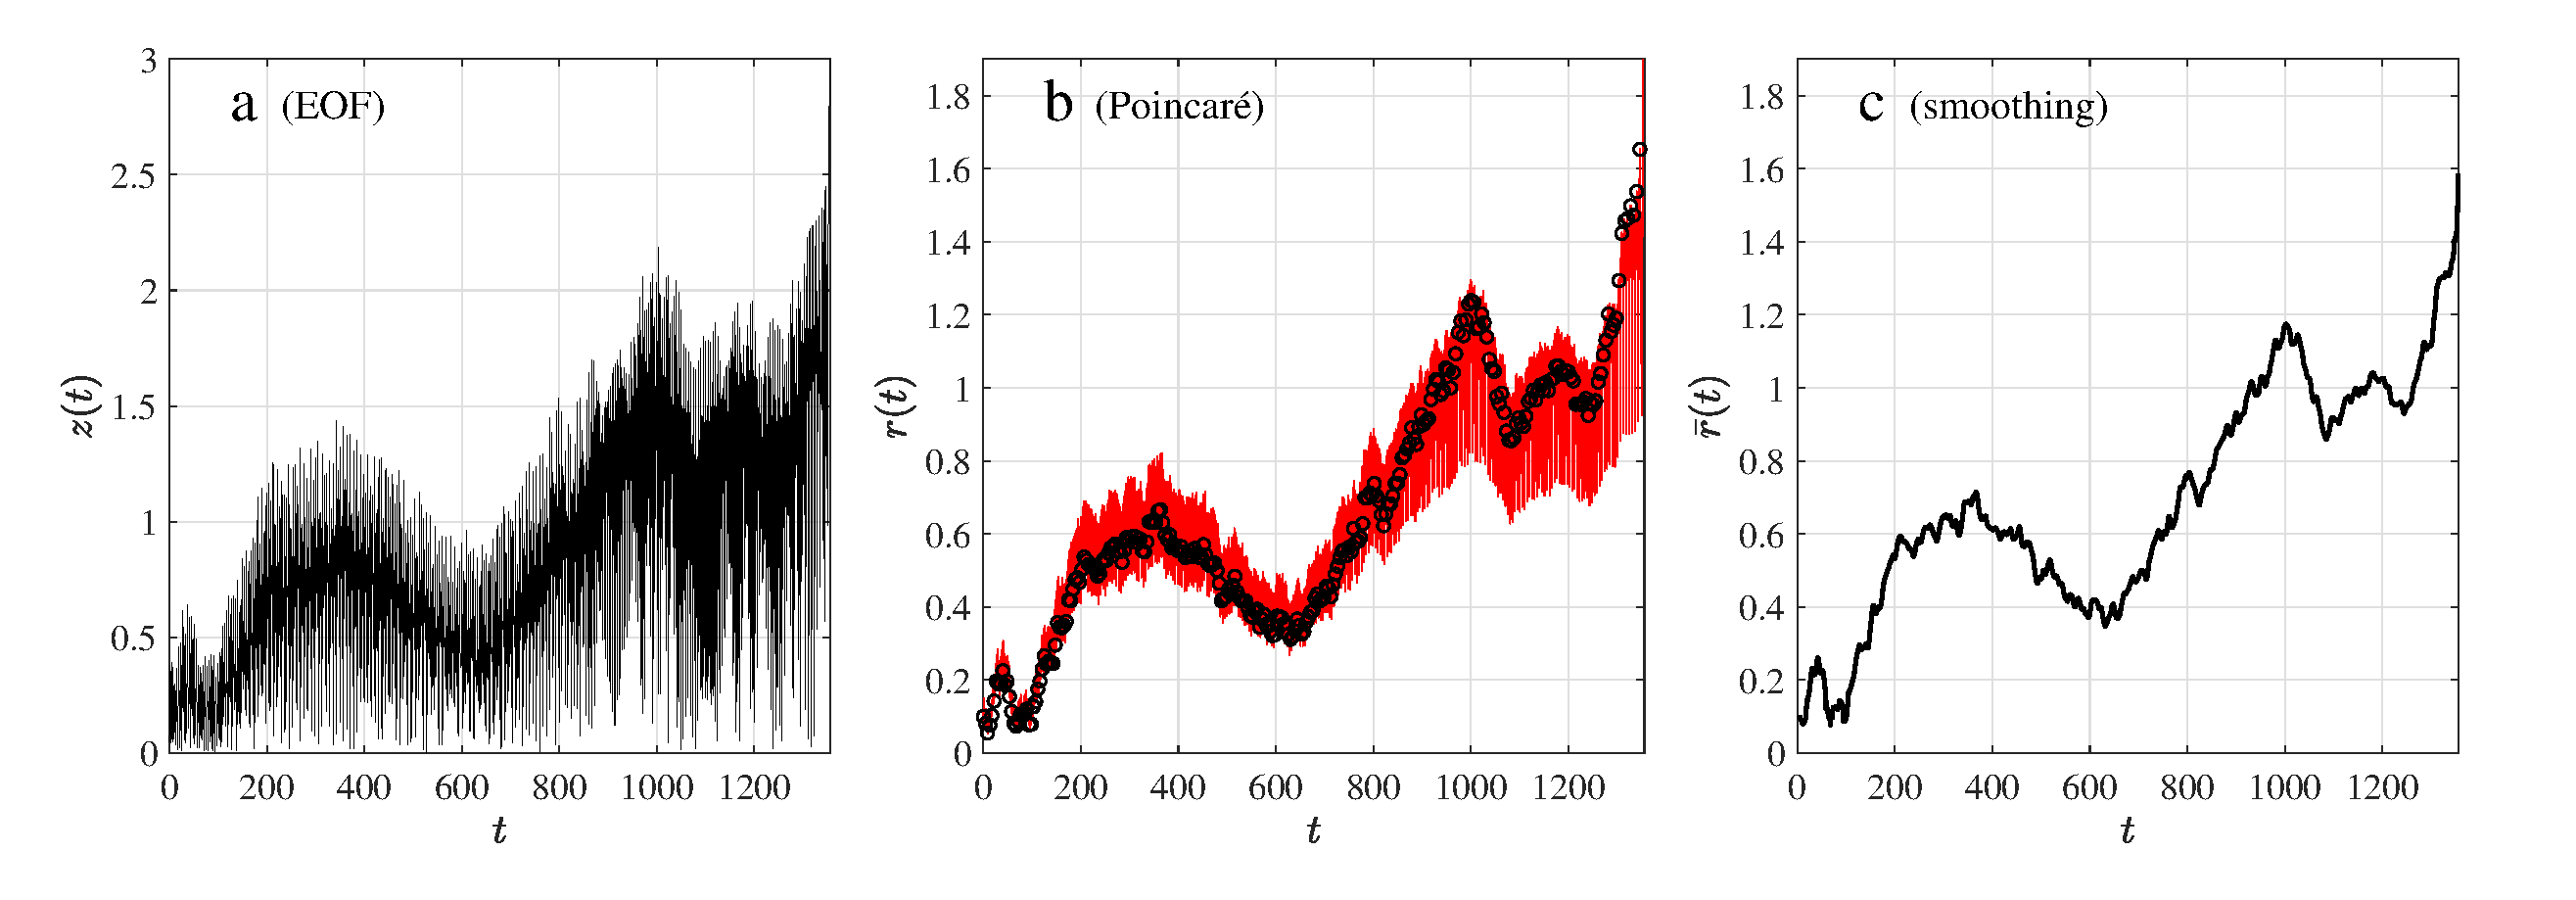
\includegraphics[width = 0.9\columnwidth]{periodicity_3Interpretations}
	\caption{\Red{Three separate interpretations of the System A time series in $x$ and $y$. Panel {\bf a}: the time series are combined using the EOF method to obtain a time series in a single variable. Panel {\bf b}: the radius $R$ (red) and also the Poincar\'{e} map of return points (black circles). Panel {\bf c}: a smoothing applied to the radius where the radius is averaged over each orbit.
	}}
	\label{fig:2D:periodicity:3Interpretations}
\end{figure}


\subsection{Results}
\label{subsec:2D:periodic_orbit:results}
{\Red{
In figure~\ref{fig:2D:periodicity:integration} one integration of System A is presented. We use system equations~\ref{eqn:2D:homoclinicSystem_again} with the standard deviation of both noise terms $\eta^{(x)}$ and $\eta^{(y)}$ set as 0.1. In order to simplify the calculations involved in the two methods described above, we make a simple change of coordinates so that the stable centre is at the origin and the saddle point at $(-2\sqrt{\alpha}, 0)$ is moving towards it as $\alpha$ goes towards zero. Also marked in figure~\ref{fig:2D:periodicity:integration} are the Poincar\'{e} return points, where the system crosses the negative $x$ axis once on each orbit. 

The system is integrated (using the Milstein method) with a time step $\Delta t = 0.01$ in the range $t\in[0,10^4]$, a significantly longer time period than was used in the analysis in section~\ref{sec:2D:MethodsApplied} (see figures~\ref{fig:2D:Homoclinic3D}, \ref{fig:2D:HomoclinicIndicators}). Accordingly, the parameter $\alpha$ is varied more slowly, according to the formula
	\begin{equation}
		\alpha(t) = 1-10^{\m4}t,
	\end{equation}
so that the bifurcation does not occur until $t=10^4$. The initial value of $\alpha$ is therefore $1$, and we use an initial point $(x,y)=(-0.1,0)$ so that the system begins by orbiting the centre at a radius $\approx 0.1$. The observed tipping point therefore occurs earlier than $t=10^4$ since the system will cross the saddle node and `blow up' before the two stable points meet. We disregard any part of the time series after $r>5$. In this particular integration, the system began to diverge at around $t=1400$. 

In figure~\ref{fig:2D:periodicity:3Interpretations} three separate interpretations of the system time series are presented. In panel {\bf a} the time series in $x$ and $y$ are combined using the EOF method to obtain a time series in a single variable. In panel {\bf b} we plot the radius $R$ over time and also the Poincar\'{e} map where the radius is recorded only at the return points. In panel {\bf c}, then, the smoothing method, as described above, has been applied to the data. 

The resulting time series from all three methods were subject to the PS, DFA and ACF1 indicators, as shown in figure~\ref{fig:2D:periodicity:crap_results}. The ACF1 indicator appears to provide the expected EWS when applied to the dimension-reduced, EOF time series, but no clear EWS is observable in any of the indicators applied to the time series produced by either the Poincaré map method or the periodic smoothing technique. 
}}

\begin{landscape}
	\begin{figure}
		\centering
		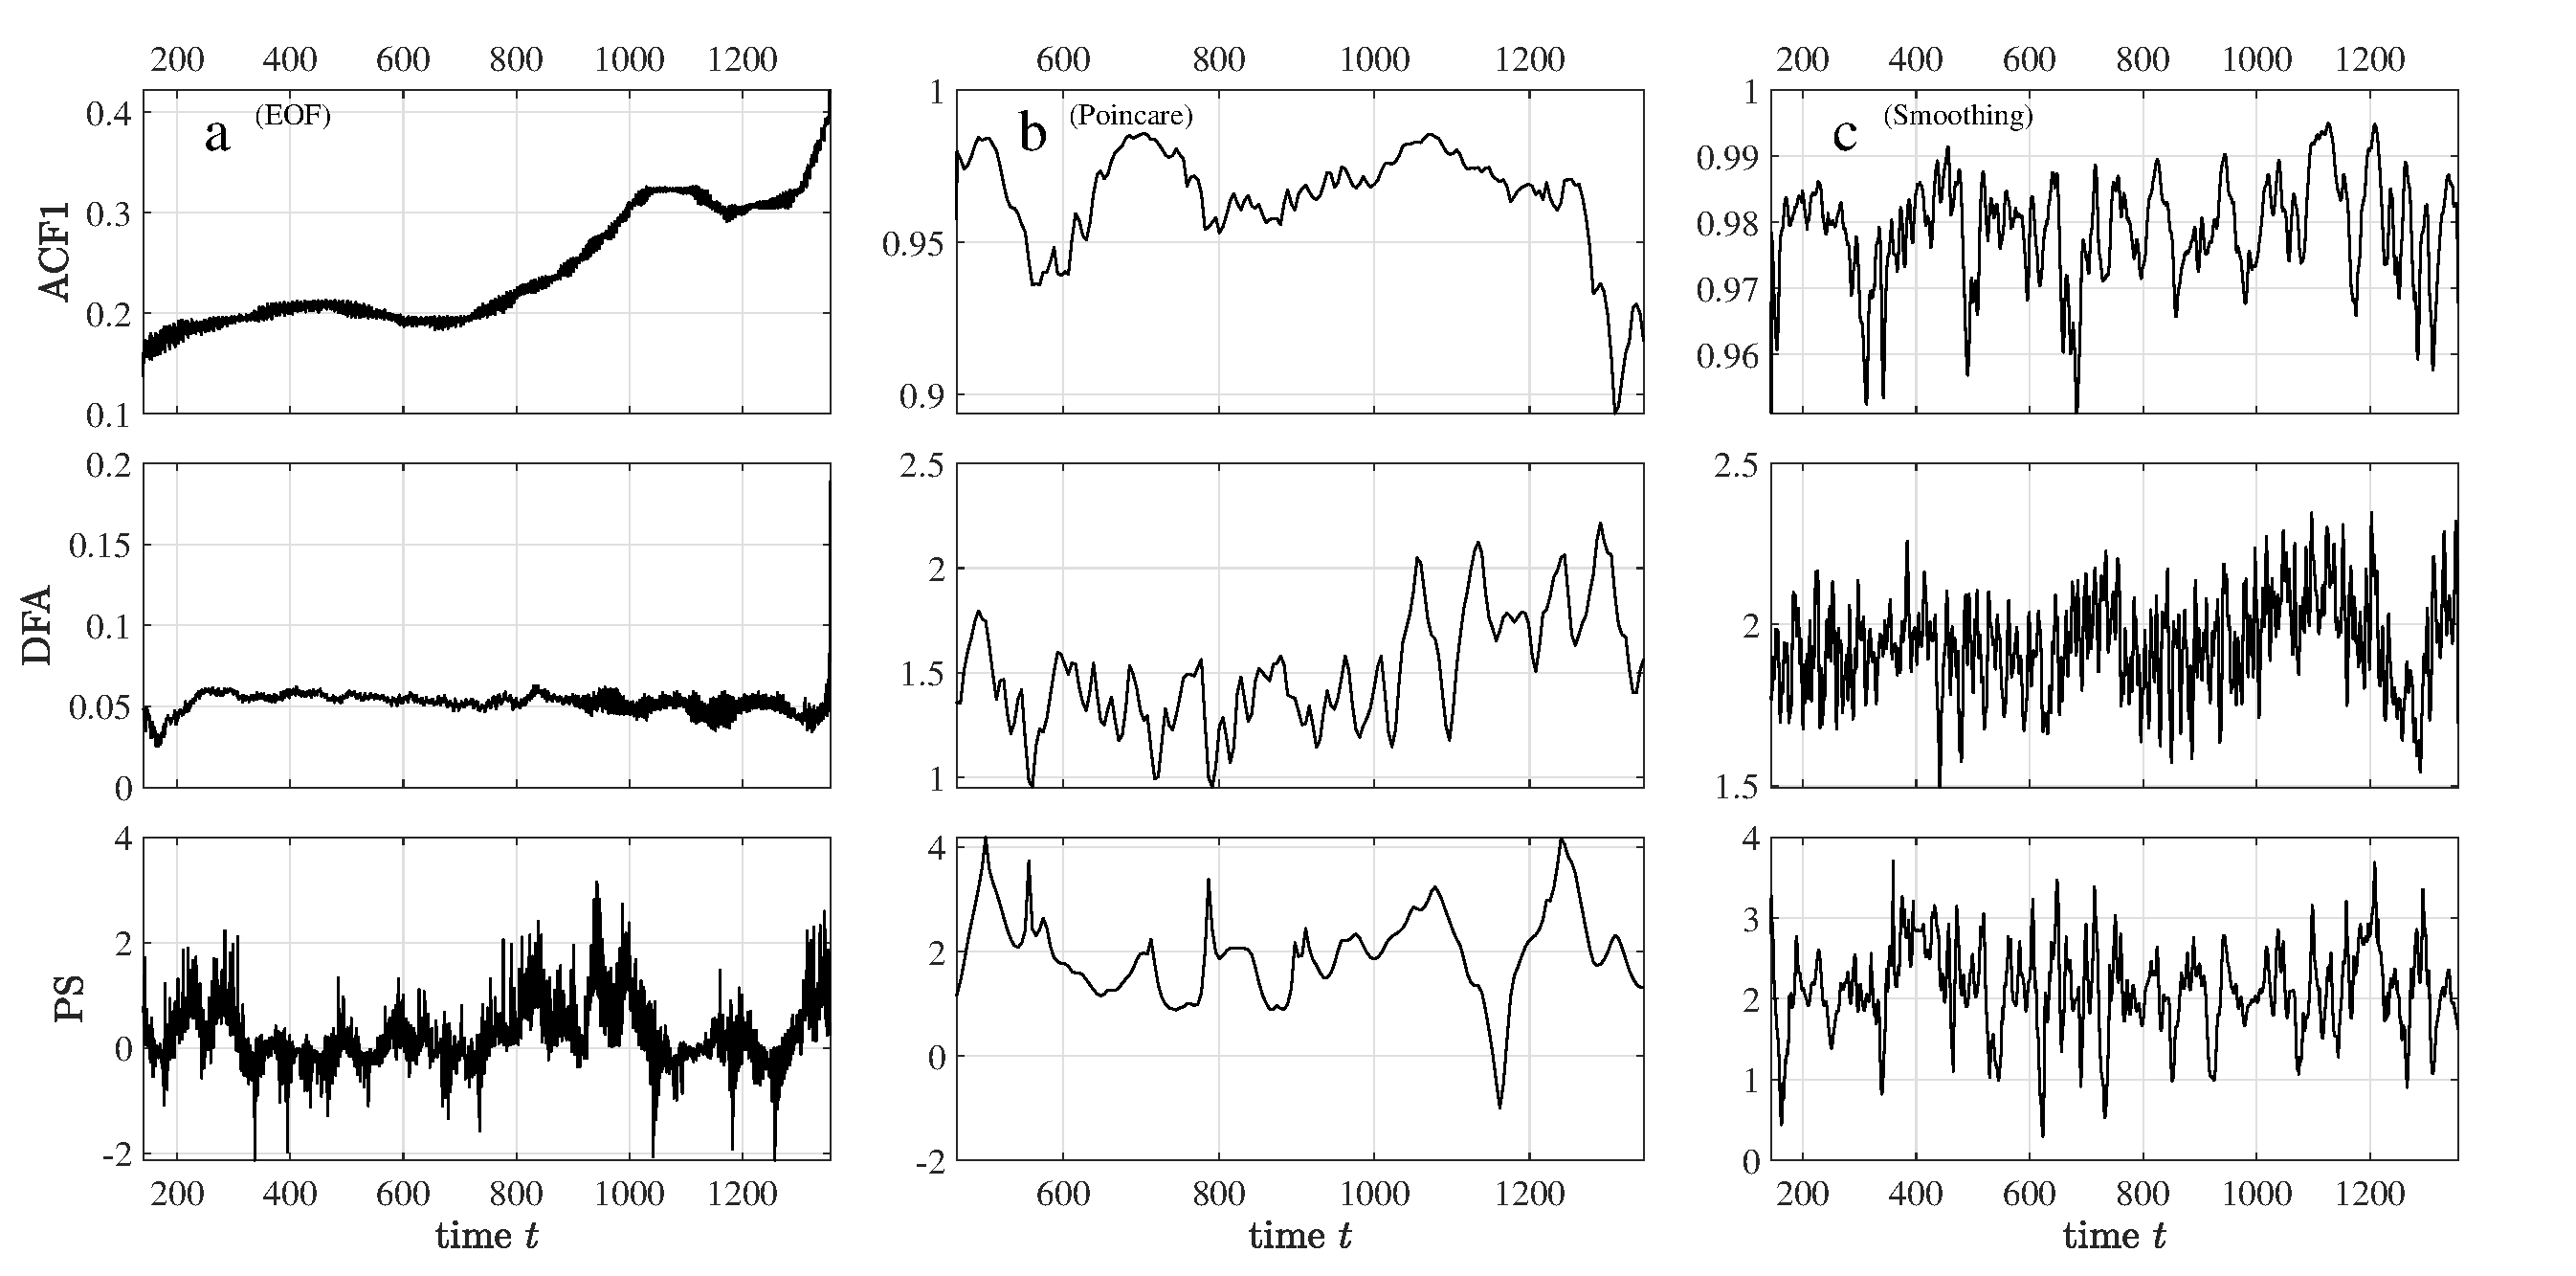
\includegraphics[width=\linewidth,keepaspectratio]{periodicity_results}
		\caption{\Red{ The ACF1 (top row), DFA (middle row) and PS (bottom row) indicators are calculated for the one dimensional time series resulting from each of the three methods illustrated in figure~\ref{fig:2D:periodicity:3Interpretations}: The EOF method (column {\bf a}), the Poincaré map approach (column {\bf b}) and the smoothing applied to the radius (column {\bf c}). We note that neither the Poincaré map nor the smoothing approaches result in any distinguishable EWS in any of the indicators.
		}}
		\label{fig:2D:periodicity:crap_results}
	\end{figure}
\end{landscape}

\section{Justification of EOF dimension reduction}
\label{sec:2D:EOF-justification}

In this section we attempt to justify the use of EOF for dimension reduction in an early warning signal context, as presented in section~\ref{sec:2D:EOF}. By taking the first EOF score of a set of time series, one is projecting on the basis such that the variance is maximised. However, one may favour a dimension which happens to be noisy, having a large variance but no interesting features indicative of a tipping point, whereas viewing the data set along another dimension, which contains lower variability, may yield a useful early warning signal. It is clear that including a single time series composed of white noise with very large variance will make the first EOF score useless. It should be hoped that such cases can be removed before applying the EOF method. However, even in less artificial cases, it is not obvious that viewing a system along a dimension such that the variance is maximised will provide the best EWS in a tipping points context. {\Red{ It may be the case that, in one projection, the variance in the system is large, but constant. In another projection the variance may be small, but \emph{increasing}. The EOF method will give the former projection, since it finds the projection such as to maximise the variance. However, in the context of tipping points, one would of course prefer the latter since it is only the \emph{increase in variance} which can be a useful EWS. The same argument may be made for autocorrelation, if an alternative EOF method sought to maximise autocorrelation rather than variance.
}}

{\Red{The analysis and results presented in this section have previously been presented in \cite{prettyman2019}.}}

\subsubsection{The hypothesis}
\label{sub:EOF-hypothesis}
The essential hypothesis relied upon when using EOF for dimension reduction prior to detecting an EWS, is that the basis in which the variance is maximised (using the EOF method) is similar to the basis in which the \emph{increase in the variance} is maximised. To investigate this hypothesis we consider the $P$-dimensional discrete-time dynamical system $\x_n$ described by 
	\begin{equation}
	\x_{n} = B\x_{n-1} + S\etab_n,
	\label{eqn:EOF-exampleSystem}
	\end{equation}
where $B$, $S$ are symmetric $P\times P$ matrices and the $\etab_n$ are column vectors with each element being independent Gaussian white noise. If $\x$ is one-dimensional ($P=1$), then the system is an AR(1) model. If $P>1$, one may want to study only the first EOF score in the hope that this captures most of the interesting behaviour of the system \citep{held2004}. 

In the simple case where $S$ is the zero matrix, we observe that, as $n$ goes to infinity, for each eigenvalue $\lambda_k$ of $B$ such that $|\lambda_k|<1$, the system goes to zero in the direction of the corresponding eigenvector. Similarly, for each eigenvalue $\lambda_k$ of $B$ such that $|\lambda_k|>1$, the system goes to infinity in the direction of the corresponding eigenvector. 

In this section we consider contracting systems, where all eigenvalues have magnitude less than one. In this case, we have a system which spirals towards zero, and approaches zero fastest in the direction of the eigenvector corresponding to the smallest eigenvalue. We then consider a matrix $B$ constructed such that one of its eigenvalues $\lambda_1$ increases over time, so that there is a tipping point at $\lambda_1=1$ when the system diverges to infinity in the direction of the eigenvector corresponding to $\lambda_1$. It is in the direction of this eigenvector that the tipping point will be most visible and, therefore, projecting the system onto this eigenvector will give the one-dimensional system in which detecting the tipping point will be easiest. If dimension reduction using the EOF method is to be used prior to using one-dimensional EWS methods, one would expect the vector onto which we project the system (the first column of $W$, see section \ref{sec:2D:EOF}), to be in the same direction as the eigenvector of $B$ corresponding to the eigenvalue which is approaching the value one.

This becomes more obvious if we say that $B$ is diagonal, which is equivalent to saying that $B$ is diagonalisable, and $S=0$. Say $B=\text{diag}(b_1, b_2, ..., b_n)$, then $b_1$, $b_2$, ..., $b_n$ are the eigenvalues of $B$ and the system becomes $P$ separate one-dimensional systems,
\begin{equation}
\x_n^{(i)} = b_i^n \x_{n-1}^{(i)}\, ,~~~~~~~ i=1,2,...,P.
\end{equation}
If $b_m = \min_i|b_i|$ the system will go to zero fastest in the direction of the standard basis vector $\mathbf{e}_m$, and we note that $\mathbf{e}_m$ is also the eigenvector of the diagonal $B$ corresponding to the eigenvalue~$b_m$.

\subsection{Analytic calculation of eigenvectors}
\label{sub:EOF-analysis}

In order to test the hypothesis of the EOF method, we calculate the EOF eigenvectors analytically. First, we calculate the empirical mean $\overline{\x}$ of the time series $\{\x_k\}_{k=0}^{N-1}$, defined by equation \ref{eqn:EOF-exampleSystem}, before applying the mean-centring step of the EOF method. We note that the system equation can be rewritten explicitly as
\begin{equation}
\x_k = B^k\x_0 + \sum_{j=0}^{k-1} B^{j} S \etab_{k-s},
\label{eqn:EOF-SytemRewrite1}
\end{equation}
and this can then be further rewritten to remove the dependence on $k$ from the sum:
\begin{align}
	\begin{split}
\x_k &= B^k\x_0 + \left[ \sum_{j=0}^{\infty} B^{j} S \etab_{k-j} - \sum_{j=k}^{\infty} B^{j} S \etab_{k-j}\right]\\
&= B^k\x_0 + \left[ \sum_{j=0}^{\infty} B^{j} S \etab_{k-j} - \sum_{j=0}^{\infty} B^{j+k} S \etab_{-j}\right]\\
&= \sum_{j=0}^{\infty} B^{j} S \etab_{k-j} - B^k \left(\sum_{j=0}^{\infty} B^{j} S \etab_{-j} - \x_0\right).
\label{eqn:EOF-SytemRewrite2}
\end{split}
\end{align}
There remains a dependence on $k$ inside the first sum in equation \ref{eqn:EOF-SytemRewrite2}, but this only affects the noise term and is easier to deal with. We also replace $k$ with $N_0+k$, effectively beginning our analysis of the system after $N_0$ steps, which will allow us to consider the long-term influence of the initial point $\mathbf{x}_0$. Now to find the empirical mean $\overline{\x}$, that is, we take the sum over $k$ in equation \ref{eqn:EOF-SytemRewrite2}:
\begin{align}
\begin{split}
	\overline{\x} &= \frac{1}{N}\sum_{k=0}^{N-1} \x_{N_0+k}\\
	&= \sum_{j=0}^{\infty} B^j S \frac{1}{N}\sum_{k=0}^{N-1}\eta_{N_0+k-j} - B^{N_0} \frac{1}{N}\sum_{k=0}^{N-1} B^k \left(\sum_{j=0}^{\infty} B^{j} S \etab_{-j} - \x_0\right).
\end{split}
\end{align}
Note that $\frac{1}{n}\sum_{k=0}^{n-1}\eta_{N_0+k-j} \rightarrow \mathbb{E}(\eta_0)$ since it is the empirical mean of independent noise terms, in this case the noise is Gaussian with mean zero, so we can ignore the first term. Also note that 
\begin{equation}
\sum_{k=0}^{N-1} B^k = (I-B)^{-1}(I-B^N),
\end{equation}
where $I$ is the identity matrix, thus we can write
\begin{equation}
\frac{1}{N}\sum_{k=0}^{N-1} \x_{N_0+k} =  B^{N_0} \frac{1}{N} (I-B)^{-1}(I-B^N)\left(\x_0 - \sum_{j=0}^{\infty} B^{j} S \etab_{-j} \right).
\label{eqn:EOF-simplifiedMean}
\end{equation}
Taking the $L^2$-norm of each side and noting that $\|I-B^N\|\leq 1$, we obtain
\begin{equation}
\left\|\frac{1}{N}\sum_{k=0}^{N-1} \x_{N_0+k}\right\| \leq \frac{\|B\|^{N_0}}{N} \left( \|(I-B)^{-1}\|\cdot \left\|\x_0 - \sum_{j=0}^{\infty} B^{j} S \etab_{-j} \right\| \right),
\end{equation}
and we note that the part in brackets does not depend on $N$, $N_0$ or $k$. We take the expectation of both sides and define
\begin{equation}
K := \mathbb{E}\left[ \|(I-B)^{-1}\| \left\|\x_0 - \sum_{j=0}^{\infty} B^{j} S \etab_{-j} \right\| \right]
\end{equation}
to say that for any value $c>0$ there is a choice of $N$ and $N_0$ such that
\begin{equation}
\mathbb{E}\left[\overline{\x}\right] \leq K\frac{\|B\|^{N_0}}{N} \leq c.
\end{equation}
With this choice of $N$ and $N_0$, we continue to use $\overline{\x}=0$. In effect, there exists a number $N_0$ such that after this number of iterations, the influence of the initial point $x_0$ is no longer significant. 

The covariance $C$, given by 
\begin{align}
C = \mathbb{E}\left[ \left(\x_{k+N_0} - \mathbb{E}(\x) \right) \left(\x_{k+N_0} - \mathbb{E}(\x) \right)^\top \right],
\end{align}
is calculated using the empirical mean to approximate the expected value as part of the EOF method by taking the sum over $k$. We also use the result $\overline{\x}=0$ to leave
\begin{equation}
C = \frac{1}{N}\sum_{k=0}^{N-1}\left[ (\x_{k+N_0})(\x_{k+N_0})^\top \right].
\label{eqn:EOF-simplifiedCovariance}
\end{equation}
Expanding this using equation \ref{eqn:EOF-SytemRewrite2}, most of the terms are essentially similar to the expression for $\overline{\x}$ and are similarly approximately zero for the same choice of $N$ and $N_0$. This is easily noticed if we simplify the expanded expression using
\begin{align}
\mathbf{p}_k &:= \sum_{s=0}^{\infty} B^{s} S \etab_{k-s}\,,\\
\mathbf{q} &:= \sum_{s=0}^{\infty} B^{s} S \etab_{-s} - \x_0\,,
\end{align}
which allows us to write $\x_k = \mathbf{p}_k - B^k\mathbf{q}$. The terms inside the sum in equation \ref{eqn:EOF-simplifiedCovariance} are then
\begin{equation}
(\mathbf{p}_{k+N_0})(\mathbf{p}_{k+N_0})^\top + B^{k+N_0}\mathbf{q}(B^{k+N_0}\mathbf{q})^\top - B^{k+N_0}\mathbf{q}(\mathbf{p}_{k+N_0})^\top - (\mathbf{p}_{k+N_0}) (B^{k+N_0}\mathbf{q})^\top.
\end{equation}
All terms except for the first involve multiplication by the matrix $B^{k+N_0}\mathbf{q}$, or its transpose. Taking the sum over $k$ gives the same expression for the mean $\overline{\x}$ as in equation \ref{eqn:EOF-simplifiedMean}, and we have chosen $N_0$ such that $\overline{\x}=0$. We now expand the remaining term inside the sum, that is, expand
\begin{equation}
(\mathbf{p}_{k+N_0})(\mathbf{p}_{k+N_0})^\top = \sum_{s=0}^\infty \sum_{r=0}^\infty B^s S(\eta_{k+N_0-s})(\eta_{k+N_0-r})^\top S^\top (B^\top)^r.
\label{eqn:EOF-double_sum_expansion}
\end{equation}
The expected value of the matrix $(\eta_{k+N_0-s})(\eta_{k+N_0-r})^\top$ is the zero matrix for $r\neq s$ and the identity matrix for $r=s$. Therefore
\begin{align}
\mathbb{E}\left[C\right] &= 
\mathbb{E}\left[\sum_{k=0}^{N-1}(\mathbf{p}_{k+N_0})(\mathbf{p}_{k+N_0})^\top\right]\\
&= 
\sum_{k=0}^{N-1}\mathbb{E}\left[(\mathbf{p}_{k+N_0})(\mathbf{p}_{k+N_0})^\top\right]\\
&= \sum_{k=0}^{N-1}\sum_{s=0}^\infty B^s S S^\top (B^\top)^s\\
&= \sum_{s=0}^\infty B^s S S^\top (B^\top)^s.
\label{eqn:EOF-covarianceFinal}
\end{align}

In the special case that $B = \text{diag}(b_1, b_2, ...)$ and $S = \text{diag}(s_1, s_2, ...)$, we are able to calculate the entire matrix component-wise to get
\begin{align}
\mathbb{E}([C]_{ii}) &= s_i^2\frac{1}{N-1}\sum_{r=1}^{N}\sum_{t=1}^{r} b_i^{2(t-r)}\\
&= s_i^2\frac{1}{N-1}\sum_{r=0}^{N-1}(N-r)b_i^{2r} \\
&= s_i^2\sum_{r=0}^{N}b_i^{2r} - s_i^2\sum_{r=0}^{N}\frac{r-1}{N-1}b_i^{2r}\\
&= s_i^2\sum_{r=0}^{\infty}b_i^{2r} - s_i^2\sum_{r=0}^{\infty}\frac{r-1 - (r+1)b^{2(N+1)}}{N-1}b_i^{2r}.
\end{align}
However, when substituting these diagonal matrices into our expression for the covariance matrix in equation \ref{eqn:EOF-covarianceFinal} we get simply
\begin{align}
\mathbb{E}([C]_{ii}) = s_i^2\sum_{r=0}^\infty b_i^{2r}.
\end{align}
This is because our working introduced the $N_0$ term in order to ignore the first terms of the series and approximate the mean as zero. It should be noted that equation \ref{eqn:EOF-covarianceFinal} is therefore only a first approximation to the covariance. 

We also note that the same calculation can be done with a time lag so that we are finding the covariance of $\x_k$ and $\x_{k+l}$. In this case the equation \ref{eqn:EOF-double_sum_expansion} becomes
\begin{align}
(\mathbf{p}_{k+N_0})(\mathbf{p}_{k+l+N_0})^\top = \sum_{s=0}^\infty \sum_{r=0}^\infty B^s S(\eta_{k+N_0-s})(\eta_{k+l+N_0-r})^\top S^\top (B^\top)^r,
\end{align}
and the expected value of the matrix $(\eta_{k+N_0-s})(\eta_{k+l+N_0-r})^\top$ is equal to the identity matrix when $r = s+l$, rather than $r=s$, and zero otherwise. So we have simply 
\begin{equation}
\mathbb{E}(C_{\text{lag-}l}) = \mathbb{E}\left[(\mathbf{p}_{k+N_0})(\mathbf{p}_{k+l+N_0})^\top\right] = \sum_{s=0}^\infty B^s S S^\top (B^\top)^{s+l},
\end{equation}
which is the same matrix as the regular (lag-0) covariance given in equation \ref{eqn:EOF-covarianceFinal} but right-multiplied by $(B^l)^\top$. For simplicity, we call this matrix $D$:
\begin{equation}
D:=\mathbb{E}(C) = \sum_{s=0}^\infty B^s S S^\top (B^\top)^s.
\end{equation}
This equation allows us to define $D$ intrinsically as
\begin{equation}
D = SS^\top + B D B^\top,
\end{equation}
which we can then solve component-wise. In the fairly trivial one-dimension case $d=s^2+b^2d$ we have 
\begin{equation}
d = \frac{s^2 }{1-b^2}\,.
\end{equation}
In two-dimensions we restrict our study to the case where $B$ is diagonal, which is equivalent to asking that $B$ is diagonalisable. We obtain
\begin{equation}
	D = \left[ 
	\begin{array}{cc}
	\frac{s_{12}^2+s_{11}^2}{1-b_{11}^2} & \frac{s_{12}s_{22}+s_{11}s_{21}}{1-b_{11}b_{22}}\\
	\frac{s_{12}s_{22}+s_{11}s_{21}}{1-b_{11}b_{22}} & \frac{s_{22}^2+s_{21}^2}{1-b_{22}^2}
	\end{array}
	\right],
\label{eqn:2D:B_diag}
\end{equation}
and are able to examine the eigenvalues easily because of its symmetry. The eigenvalues of a general symmetric $2\times 2$ matrix 
\begin{equation}
\left(
\begin{array}{cc}
a&b\\
b&c
\end{array}
\right)
\end{equation}
are 
\begin{equation}
\frac{1}{2}\left(a+c\pm\sqrt{(a-c)^2+4b^2}\right),
\label{eqn:EOF-generalEigenvalues}
\end{equation}
and we can see that, when matrix $D$ is substituted into this, the positive square root will give the largest (principal) eigenvalue. Note that for $b=0$ (i.e. the matrix is diagonal) the difference between the two eigenvalues is $|a-c|$, but for non-zero $b$ this difference increases, i.e. the eigenvalues become more distinct. Matrix $D$ is diagonal when two entries of $S$ are zero, not in the same column, in which case the system (equation \ref{eqn:EOF-exampleSystem}) is simply two separate AR(1) models. The eigenvector corresponding to the largest eigenvalue (taking the positive root) is 
\begin{equation}
\left[\begin{array}{c}
\frac{s_{12}^2+s_{11}^2}{1-b_{11}^2}-\frac{s_{22}^2+s_{21}^2}{1-b_{22}^2} + \sqrt{\left(\frac{s_{12}^2+s_{11}^2}{1-b_{11}^2}-\frac{s_{22}^2+s_{21}^2}{1-b_{22}^2}\right)^2+4\left(\frac{s_{12}s_{22}+s_{11}s_{21}}{1-b_{11}b_{22}}\right)^2}\\
~\\
2\left(\frac{s_{12}s_{22}+s_{11}s_{21}}{1-b_{11}b_{22}}
\right)
\end{array}\right].
\label{eqn:EOF-2x2eigenvector}
\end{equation}
This is the principal eigenvector used in the EOF method; the assumption is that projecting onto this eigenvector, which maximises variance, captures the interesting behaviour of the system. For the purpose of tipping point analysis, we would therefore expect that this eigenvector has something to do with the eigenvector corresponding to the largest eigenvalue of $B$ (closest to one), since this is the direction in which the system travels slowest to zero. A bifurcation occurs when one eigenvalue approaches one. 

Without loss of generality, we assume that the first eigenvalue of $B$ is approaching one; since $B$ is diagonal this is equal to the first entry of $B$, $b_{11}$, and the corresponding eigenvector is the standard basis vector $\mathbf{e}_1 = [1,0]^\top$.
We make the choice that $b_{11}\approx 1$ (from below), then 
$1-b_{11}$ is very small. We are therefore inclined to expand the terms in the principal eigenvector (equation~\ref{eqn:EOF-2x2eigenvector}) in leading order terms of $(1-b_{11})$, allowing us simplify the expression by ignoring negligible terms. The objective is to expand the square root
\begin{equation}
	Q := \sqrt{\left(\frac{s_{12}^2+s_{11}^2}{1-b_{11}^2}-\frac{s_{22}^2+s_{21}^2}{1-b_{22}^2}\right)^2+4\left(\frac{s_{12}s_{22}+s_{11}s_{21}}{1-b_{11}b_{22}}\right)^2}.
\end{equation}
To simplify the working we make the following substitutions:
	\begin{align}
	\begin{split}
		\varepsilon &:=1-b_{11},\\
		p &:= s_{11}^2+s_{12}^2,\\
		q &:= s_{21}^2+s_{22}^2, \\
		r &:= s_{12}s_{22}+s_{11}s_{21}.
	\end{split}
	\end{align}
The expression then becomes
	\begin{align}
	\begin{split}
		Q =& \sqrt{\left(\frac{p}{\varepsilon(1+b_{11})}-\frac{q}{1-b_{22}^2}\right)^2+4\left(\frac{r}{1-(1-\varepsilon) b_{22}}\right)^2}\\
		=& \frac{1}{\varepsilon}\sqrt{\frac{p^2}{(1+b_{11})^2}-\varepsilon\frac{2pq}{(1+b_{11})(1-b_{22}^2)}-\varepsilon^2\frac{q^2}{(1-b_{22}^2)^2}+\varepsilon^2\frac{4r^2}{(1-(1-\varepsilon) b_{22})^2}} \,\, .
	\end{split}
	\end{align}
Concentrating on the final term inside the square root, we use the Taylor expansion of $1/(1+x)$ to obtain
	\begin{align}
	\begin{split}
		\frac{1}{1-(1-\varepsilon) b_{22}} &= 1+(1-\varepsilon) b_{22}+(1-\varepsilon)^2 b_{22}^2+...\\
		&=\frac{1}{1-b_{22}} -
		\varepsilon\sum_{k=1}^\infty kb_{22}^k + \varepsilon^2\sum_{k=2}^\infty\left(\begin{array}{c}	k\\2\end{array}\right)b_{22}^k + \mathcal{O}(\varepsilon^3) \,\, ,
	\end{split}
	\end{align}
	and therefore
	\begin{equation}
		\varepsilon^2\frac{4r^2}{(1-(1-\varepsilon) b_{22})^2} = \varepsilon^2\frac{4r^2}{(1-b_{22})^2}+\mathcal{O}(\varepsilon^3) \,\, .
	\end{equation}
Then we can return to our square root:
{\small
	\begin{align}
	\begin{split}
		Q&= \frac{1}{\varepsilon}\sqrt{\frac{p^2}{(1+b_{11})^2}-\varepsilon\frac{2pq}{(1+b_{11})(1-b_{22}^2)}+\varepsilon^2\left[ \frac{4r^2(1+ b_{22})^2 -  q^2 }{(1-b_{22}^2)^2} \right] + \mathcal{O}(\varepsilon^3)}\\
		&= \frac{p}{\varepsilon (1+b_{11})} \sqrt{1+\varepsilon\frac{-2q(1+b_{11})}{p(1-b_{22}^2)}+\varepsilon^2(1+b_{11})^2\left[ \frac{4r^2(1+ b_{22})^2 -  q^2 }{p^2(1-b_{22}^2)^2} \right] + \mathcal{O}(\varepsilon^3)}\\
		&= \frac{p}{\varepsilon (1+b_{11})}\left[1+
		\varepsilon\frac{-q(1+b_{11})}{p(1-b_{22}^2)}+\varepsilon^2\frac{(1+b_{11})^2}{2}\left[ \frac{4r^2(1+ b_{22})^2 -  q^2 }{p^2(1-b_{22}^2)^2}\right] - 
		\right. \\
		& \qquad\qquad\qquad\qquad\qquad\qquad\qquad\qquad\qquad \quad \left.
		-\frac{1}{8}\left(\varepsilon\frac{-2q(1+b_{11})}{p(1-b_{22}^2)} \right)^2 + \mathcal{O}(\varepsilon^3)
		\right] \\
		&= \frac{p}{\varepsilon (1+b_{11})}\left[1+
		\varepsilon\frac{-q(1+b_{11})}{p(1-b_{22}^2)}+
		\varepsilon^2 \left[ \frac{4r^2(1+ b_{22})^2(1+b_{11})^2 -  q^2(1+b_{11})^2 }{2p^2(1-b_{22}^2)^2}\right] \right. \\
		&\qquad\qquad\qquad\qquad\qquad\qquad\qquad\qquad\qquad  \qquad\left.
		-\varepsilon^2\left[\frac{q^2(1+b_{11})^2}{2p^2(1-b_{22}^2)^2}\right]
		+ \mathcal{O}(\varepsilon^3)
		\right]\\
		&= \frac{p}{\varepsilon (1+b_{11})}\left[1+
		\varepsilon\frac{-q(1+b_{11})}{p(1-b_{22}^2)}+
		\varepsilon^2(1+b_{11})^2 \left[ \frac{4r^2(1+ b_{22})^2 -  2q^2 }{2p^2(1-b_{22}^2)^2}\right]
		+ \mathcal{O}(\varepsilon^3)
		\right]\\
		&=
		\frac{p}{\varepsilon (1+b_{11})} + 
		\frac{-q}{(1-b_{22}^2)}+
		\varepsilon(1+b_{11}) \left[ \frac{2r^2(1+ b_{22})^2 -  q^2 }{p(1-b_{22}^2)^2}\right]
		+ \mathcal{O}(\varepsilon^2)\\
		&=
		\frac{p}{(1-b_{11}^2)} + 
		\frac{-q}{(1-b_{22}^2)}+
		(1-b_{11}^2) \left[ \frac{2r^2(1+ b_{22})^2 -  q^2 }{p(1-b_{22}^2)^2}\right]
		+ \mathcal{O}(\varepsilon^2).
	\end{split}
	\end{align}
}
We can now substitute this expansion of $Q$ for the square root term in the first component of the principal eigenvector (equation~\ref{eqn:EOF-2x2eigenvector}), which becomes
	\begin{equation}
		\frac{2p}{(1-b_{11}^2)} + 
		\frac{-2q}{(1-b_{22}^2)}+
		(1-b_{11}^2) \left[ \frac{2r^2(1+ b_{22})^2 -  q^2 }{p(1-b_{22}^2)^2}\right]
		+ \mathcal{O}((1-b_{11})^2),
	\end{equation}
or simply
	\begin{equation}
		\frac{2p}{(1-b_{11}^2)} + 
		\frac{-2q}{(1-b_{22}^2)}
		+ \mathcal{O}((1-b_{11})).
	\end{equation}
A similar treatment of the second eigenvector component yields
	\begin{align}
		\frac{2r}{1-b_{11}b_{22}} & = 2r\left[\frac{1}{1-b_{22}} -
		\varepsilon\sum_{k=1}^\infty kb_{22}^k + \varepsilon^2\sum_{k=2}^\infty\left(\begin{array}{c}k\\2\end{array}\right)b_{22}^k + \mathcal{O}(\varepsilon^3)
		\right]\\
		& = 2r\left[\frac{1}{1-b_{22}} -
		\varepsilon\frac{b_{22}}{(1-b_{22})^2}
		\right]
		+ \mathcal{O}(\varepsilon^2)\\
		& = \frac{2r(1 - 2b_{22} + b_{11}b_{22})}{(1-b_{22})^2}
		+ \mathcal{O}((1-b_{11})^2)\\
		& = \frac{2r}{1-b_{22}}+ \mathcal{O}((1-b_{11})).
	\end{align}
Thus, if we ignore terms in $\mathcal{O}(1-b_{11})$, the principal eigenvector in equation~\ref{eqn:EOF-2x2eigenvector} becomes
\begin{equation}
\left[\frac{s_{12}^2+s_{11}^2}{1-b_{11}^2}-\frac{s_{22}^2+s_{21}^2}{1-b_{22}^2} ~,~\frac{s_{12}s_{22}+s_{11}s_{21}}{1-b_{22}}
\right]^\top,
\label{eqn:2D:EOFeigenVector}
\end{equation}
which, since $1/(1-b_{11}^2)$ is very large, is approximately equivalent to $[1,0]^\top$ as expected. If $S$ is diagonal ($s_{12}=s_{21}=0$) then the vector is actually equivalent to $[1,0]^\top$, in this situation the two system variables are actually separate one-dimensional AR(1) models, since $B$ is also diagonal. However, if $s_{11},s_{12}$ are very small and $s_{21},s_{22}$ are very large, it may not be true that the eigenvector is approximately in the direction $[1,0]^\top$. This implies that there is very large variability in the second component of the system (in the direction of $[0,1]^\top$), and so this exception is predicted by our knowledge of the EOF method. 

We have considered the expected value of the covariance matrix, since the noise will cause every realisation of the system to be different. This analysis is also intended to tell us something general about the validity of using dimension reduction by the EOF method prior to using tipping point analysis techniques. The method must be valid where the entries of $S$ are large, giving large variability due to noise, or in situation when given time series data of unknown origin which resembles the output of the general system in equation~\ref{eqn:EOF-exampleSystem}. In these situations the covariance matrix $C$ obtained from the data by the EOF method may be significantly different to the expectation $D = \mathbb{E}(C)$, in which case it may be uncertain which is truly the principal eigenvalue, especially when the eigenvalues are very similar. Equation~\ref{eqn:EOF-generalEigenvalues} tells us that the difference between the eigenvalues is smallest when the covariance matrix is diagonal, i.e. when the system is reducible to separate AR(1) models, and that the difference increases as the off-diagonal entries of $S$ increase, i.e. as the system becomes more strongly coupled.

\subsection{Numerical verification}
\label{sub:EOF-verification}
The analysis in section \ref{sub:EOF-analysis} makes some assumptions to aid the calculations. In particular, only two-dimensional systems are considered when calculating the eigenvectors of the covariance matrix. In this section we provide numerical experiments to further validate the conclusions of section \ref{sub:EOF-analysis} and also to provide some insight into three- and four-dimensional systems. 

\subsubsection{Two-dimensional system}
We first consider the two-dimensional system 
\begin{equation}
\x_{k} = \Lambda\x_{k-1} + S\etab_k,
\label{eqn:EOF-2DbasicSystem}
\end{equation}
where $\etab_k$ is a white noise vector and $\Lambda=\text{diag}(\lambda_1, \lambda_2)$ is diagonal. $\lambda_2 = 0.9$ and $\lambda_1$ is made to approach one from below:
\begin{equation}
	\lambda_1(k) = 0.9+10^{-6}k,
\end{equation}
so that $\lambda_1=\lambda_2$ at $k=0$, and at $k=10^5$ a bifurcation occurs as the system tips from convergence to divergence, diverging to infinity in the $x$-direction, i.e. in the direction of $(\pm 1,0)^\top$. In the previous section we concluded that the nature of the matrix $S$, specifically the values on the off-diagonal, determines the effectiveness of the EOF method in this context. As an illustration, we initially consider two extreme cases: 
\begin{enumerate}
	\item The two variables are entirely uncoupled:\begin{equation}
	\label{eqn:2D:uncoupledMatrix}
		S_1 = \frac{1}{20}\left(\begin{array}{cc}
		1 & 0 \\
		0 & 1
		\end{array}\right).
	\end{equation}
	\item The two variables are coupled:\begin{equation} 
	\label{eqn:2D:coupledMatrix}
		S_2 = \frac{1}{20}\cdot\frac{1}{\sqrt{2}}\left(\begin{array}{cc}
		1 & 1 \\
		1 & 1
		\end{array}\right).
	\end{equation}
\end{enumerate}
 The factor $1/\sqrt{2}$ in $S_2$ is to ensure that the standard deviation of the noise is the same in both cases. Na\"ively, we may expect that the leading EOF eigenvector will be similar to $(\pm 1,0)^\top$ since this is the direction in which the divergence happens, or, before the bifurcation, the direction in which the convergence is weakest and therefore the direction with the longest recovery time after a perturbation from the equilibrium. This may be true eventually but not when $\lambda_1$ and $\lambda_2$ are very close. According to equation~\ref{eqn:EOF-2x2eigenvector}, the eigenvector, when using the identity matrix $S_1$, will be 
\begin{equation}
	\left[\begin{array}{c}
	\frac{1}{1-\lambda_1^2}-\frac{1}{1-0.9^2}\\
	0
	\end{array}\right],
\label{eqn:2D:S1expected_eigenvector}
\end{equation}
which is in the direction $(\pm 1,0)^\top$ for $\lambda_1\neq 0.9$, but is the zero vector when $\lambda_1= 0.9$. At this point, the EOF eigenvector is determined only by the noise, and therefore the angle of that vector will be random in the range $[-\pi/2, \pi/2]$, with mean zero. The angle will tend to zero (i.e. the EOF eigenvector will approach $(1,0)^\top$) as the difference $|\lambda_1-0.9|$ is sufficiently large that the EOF method is able to distinguish the effect upon the system from the noise. 

When using the matrix $S_2$ we will have the vector
\begin{equation}
\left[\begin{array}{c}
\frac{1}{1-\lambda_1^2}-\frac{1}{0.19} + \sqrt{\left(\frac{1}{1-\lambda_1^2}-\frac{1}{0.19}\right)^2+\left(\frac{2}{1-0.9\lambda_1}\right)^2}\\
~\\
\frac{2}{1-0.9\lambda_1}
\end{array}\right]\,,
\label{eqn:2D:S2expected_eigenvector}
\end{equation}
which is in the direction $(1,1)^\top$ for $\lambda_1=0.9$ and approaches $(1,0)^\top$ as $\lambda_1\rightarrow 1$ as the $1/(1-\lambda_1^2)$ term becomes very large. The angle of this vector will therefore start as $\theta_\text{eig} = \pi/4$ when $k=0$ (i.e. $\lambda_1=0.9$) and tends towards zero as $k$ increases. 

Using both of these matrices $S_1$ and $S_2$ we calculate the terms $\x_k$ up to the point of the bifurcation ($k=10^5$). For each of the resulting series we perform the EOF analysis on 200 half-overlapping segments of length $10^3$, in order to see how the EOF eigenvectors change as $k$ increases. In each segment the angle variable of the EOF eigenvector is calculated.

Figure~\ref{fig:2D:EOFtest_extreme_simple} shows the result when using $S_1$ (panel \textbf{a}) and $S_2$ (panel \textbf{b}). 
\begin{figure}
	\centering
	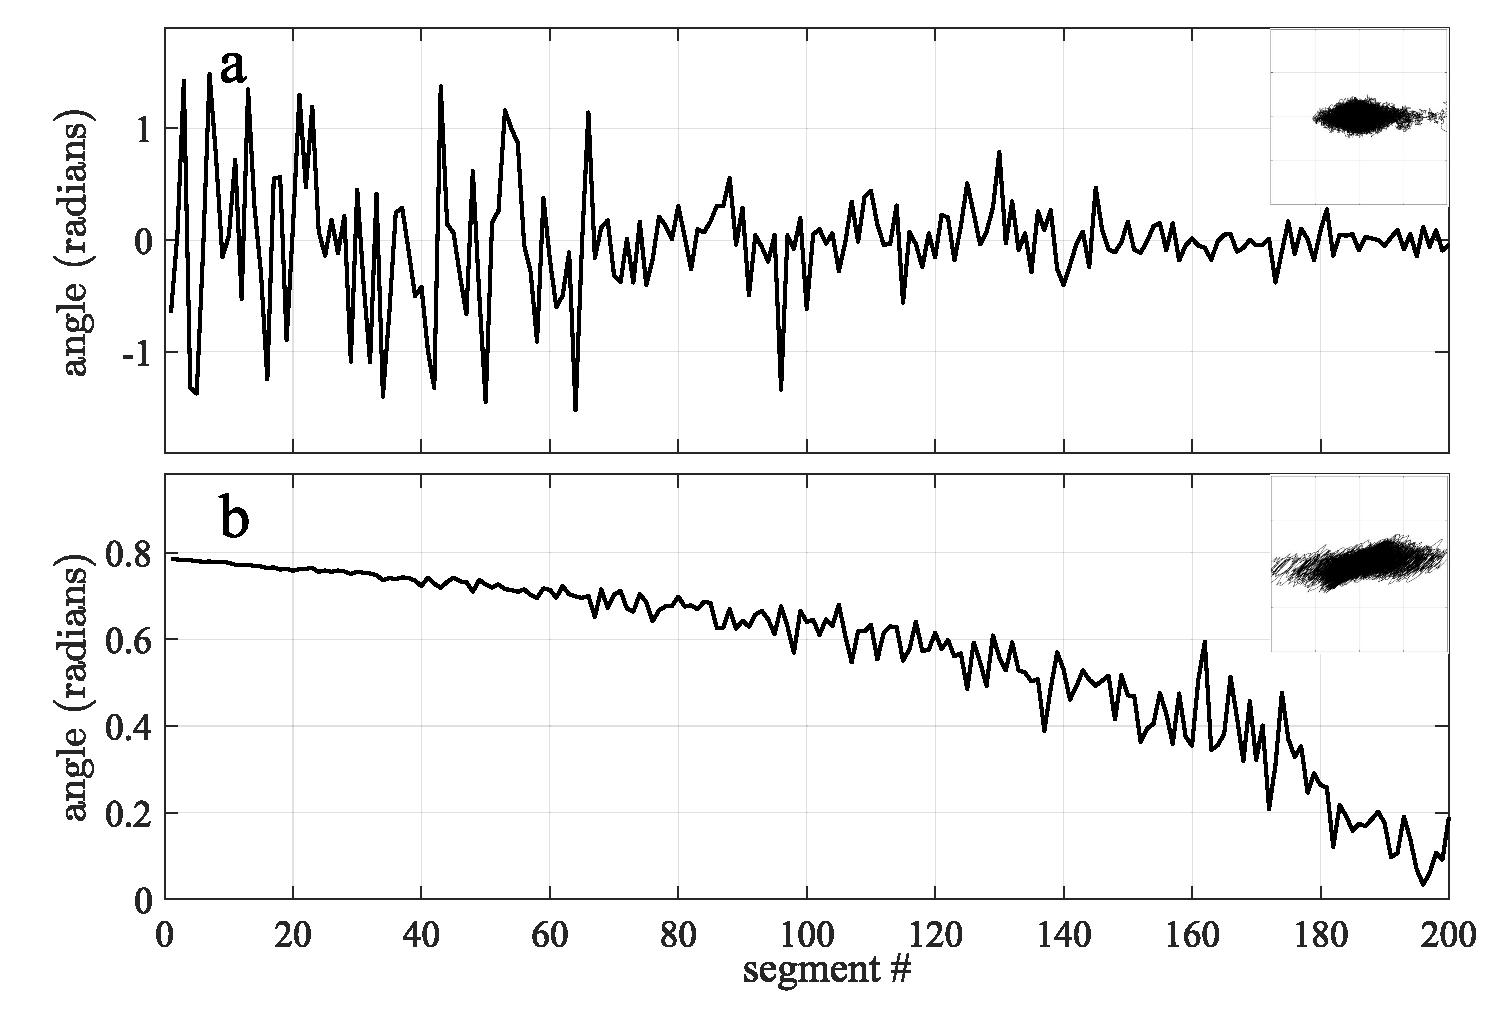
\includegraphics[width = 0.9\columnwidth]{EOFtest_extreme_simple2}
	\caption{The angle variable of the EOF eigenvector calculated in 200 overlapping segments of length $10^3$. Two cases of the system in equation~\ref{eqn:EOF-2DbasicSystem} are considered: using $S_1$ (panel \textbf{a}) and using $S_2$ (panel \textbf{b}), see equations~\ref{eqn:2D:uncoupledMatrix} and~\ref{eqn:2D:coupledMatrix}. The series itself is plotted, in each case, in the insert at the top-right of the panel, both $x$ and $y$ axes range from $-2$ to $2$.
		\label{fig:2D:EOFtest_extreme_simple}}
\end{figure}
We see that the nature of the matrix $S$ does affect the EOF projection. When the two systems are uncoupled (i.e. the two variables are two separate AR(1) models) the angle of the eigenvector is apparently random at first when $\lambda_1$ is close to the value $0.9$ but the angle converges towards zero as $\lambda_1$ goes to 1, as predicted. When the two variables are coupled, the angle variable of the EOF eigenvector starts at $\pi/2$ (for $\lambda_1=0.9$) and tends towards zero, also as predicted. 

We now perform the same analysis using a range of 30 intermediate symmetric matrices
\begin{equation}
	S^{(\phi)} = \frac{1}{20}\left(\begin{array}{cc}
	\cos(\phi) & \sin(\phi) \\
	\sin(\phi) & \cos(\phi)
	\end{array}\right),
\end{equation}
where $\phi$ varies from zero (giving the identity matrix $S_1$) to $\pi/4$ (giving the ones matrix $S_2$). For each of the 30 matrices $S^{(\phi)}$ the series $\x_k$ is calculated and the EOF eigenvector angle is found in three segments: one at the start of the series where $\lambda_1$ is close to 0.9 ($k\in[1\times 10^4,2\times 10^4]$); one in the middle of the series ($k\in[4.5\times 10^4,5.5\times 10^4]$); and one close to the bifurcation ($k\in[8\times 10^4,9\times 10^4]$). This is repeated ten times to overcome the effect of noise, and only the absolute value of the angle variable is recorded. The result is shown in figure~\ref{fig:2D:EOFtest_changeS}.
\begin{figure}
	\centering
	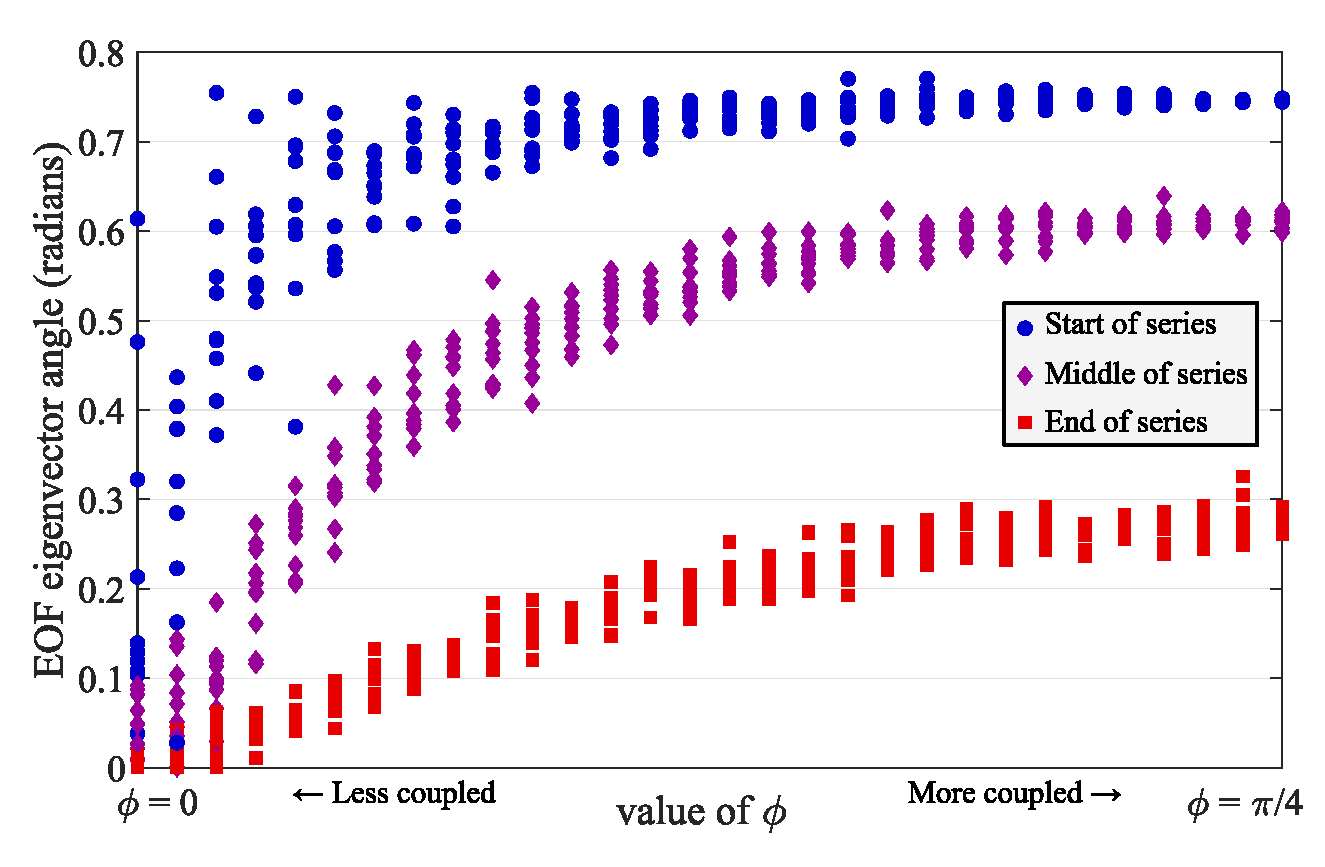
\includegraphics[width = 0.9\columnwidth]{EOFtest_changeS}
	\caption{The absolute value of the angle variable of the EOF eigenvector calculated in three segments of the series $\x_k$ (start, middle and end) using a range of matrices $S^{(\phi)}$. The series is calculated 10 times for each matrix $S^{(\phi)}$, showing the range of angles, particularly for low values of $\phi$ where the system variables are uncoupled.
		\label{fig:2D:EOFtest_changeS}}
\end{figure}
We see that the results at $\phi = 0$ (matrix $S_1$) and $\phi=\pi/4$ (matrix $S_2$) are similar to the results shown in figure~\ref{fig:2D:EOFtest_extreme_simple}, bearing in mind that, this time, the absolute angle is recorded. However, in the case of the uncoupled system (small $\phi$) there is less variability here at the start of the series than seen in figure~\ref{fig:2D:EOFtest_extreme_simple}. Rather than being distributed in the range $[0,\pi/2]$, the ‘start of series' points, which correspond to the same values of $k$ as segments numbered $20$ to $40$ in figure~\ref{fig:2D:EOFtest_extreme_simple}, do not exceed $0.8$. This is because of the larger sample used: $10^4$ points rather than $10^3$ points. Repeating the figure~\ref{fig:2D:EOFtest_extreme_simple} analysis with a larger segment size, we note that this results in a more accurate EOF projection since, with a larger sample, the effect of the system eigenvalues of the convergence or divergence is more easily distinguishable from the noise. 

We note that after about half way along the horizontal axis ($\phi>\pi/8$) there is almost no change in any of the segments. Most of the qualitative change occurs over the first six values of $\phi$ used, that is $\phi<\pi/20$, which leads us to consider the matrix 
	\begin{equation}
		S^{(\pi/20)} = \frac{1}{20}\left(\begin{array}{cc}
		0.988 & 0.156 \\
		0.156 & 0.988
		\end{array}\right).
	\end{equation}
At this level of noise (standard deviation = $1/20$) the degree to which the system variables are coupled does not qualitatively affect the EOF method beyond this point. 

\subsubsection{Three-dimensional system}
We now perform the same analysis as above with equation~\ref{eqn:EOF-2DbasicSystem} being a three dimensional system, that is, $\Lambda=\text{diag}(\lambda_1, \lambda_2, \lambda_2)$. In this system $\lambda_2 = 0.9$, and $\lambda_1$ is made to approach one from below:
	\begin{equation}
		\lambda_1(k) = 0.9+10^{-6}k\,.
	\end{equation}
We use the matrices $S_1 = \sigma I$ and $S_2 = \sigma(1/\sqrt{3}) J$ where $I$ is the identity matrix, $J$ is the ones matrix and $\sigma=1/20$ is the standard deviation. Again, the series $\x_k$ is calculated up to $k=10^5$ and the EOF eigenvector is found in overlapping sections of length 1000. This time the angle recorded is necessarily the absolute angle between the EOF eigenvector and $(1,0,0)^\top$, since a negative angle does not make sense in three dimensional space. The result is shown in figure~\ref{fig:2D:EOFtest3D_simple}. 
	\begin{figure}
		\centering
		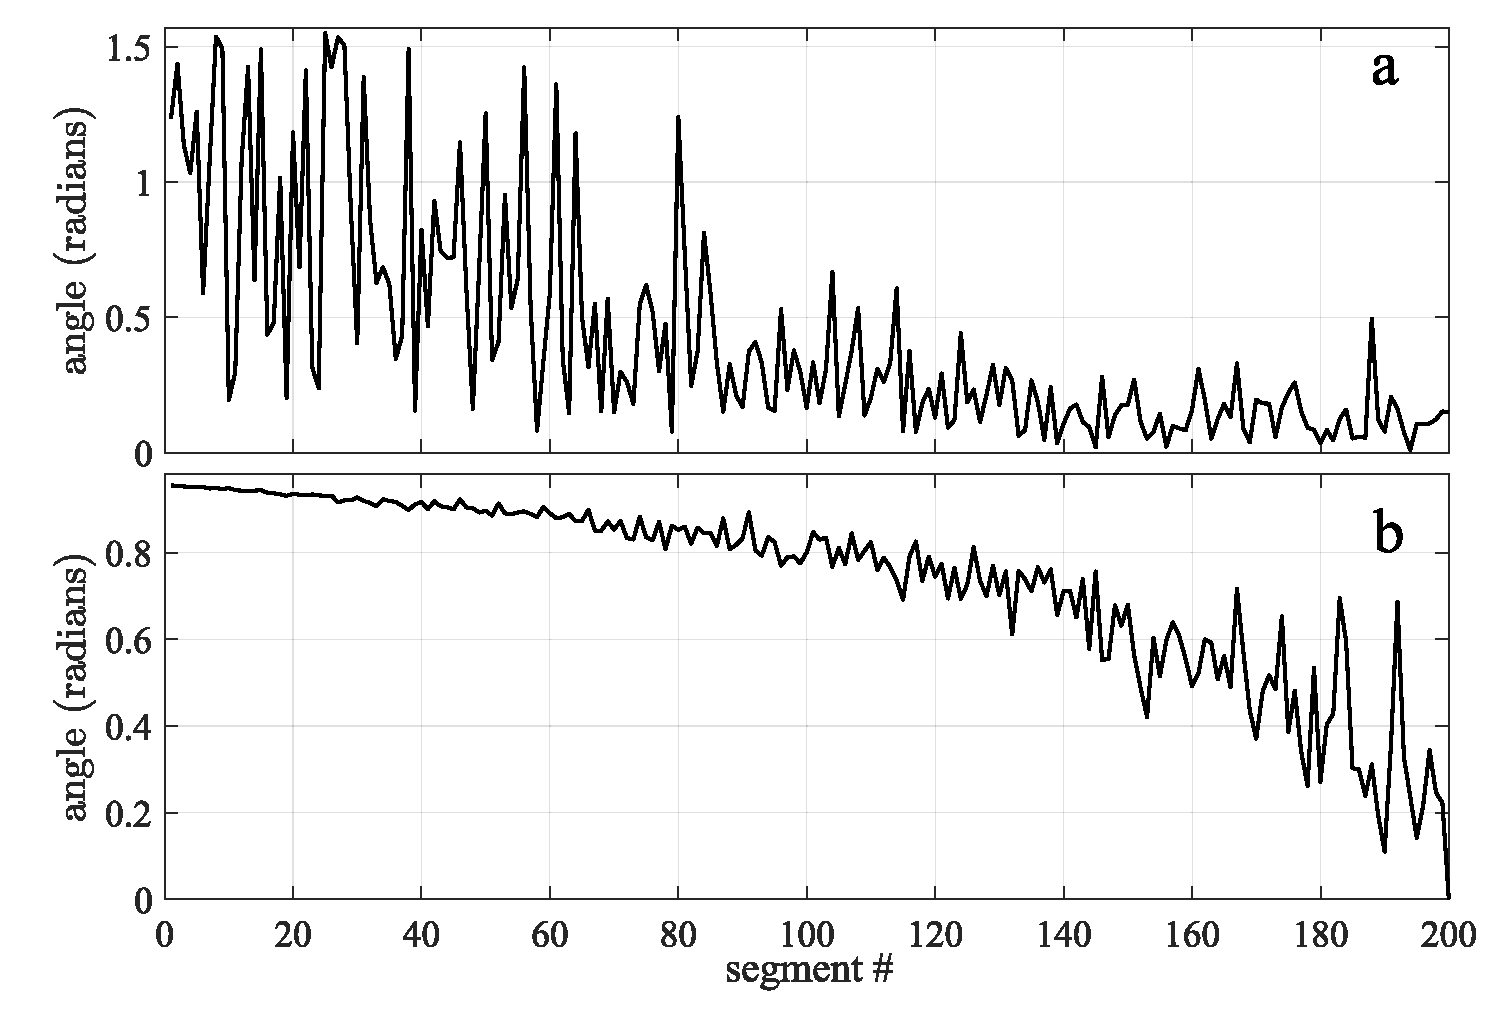
\includegraphics[width = 0.9\columnwidth]{EOFtest3D_simple}
		\caption{The angle variable of the EOF eigenvector calculated in 200 overlapping segments of length $10^3$. Two cases of the three-dimensional system in equation~\ref{eqn:EOF-2DbasicSystem} are considered: using $S_1$ (panel \textbf{a}) and using $S_2$ (panel \textbf{b}).
			\label{fig:2D:EOFtest3D_simple}}
	\end{figure}
We note the obvious similarity to figure~\ref{fig:2D:EOFtest_extreme_simple}, bearing in mind (looking at panel \textbf{a}) that the absolute value of the angle is now considered, so that the random angle will be distributed in the range $[0,\pi/2]$, and (looking at panel \textbf{b}) that the angle made by the vector $(1,1,1)^\top$ is $\arccos(1/\sqrt{3}) = 0.9553...$ which is the angle of the EOF eigenvector when $\lambda_1=0.9$. It appears that there is greater variability in the $S_2$ case close to the end of the series, but the general pattern is the same.

As a further confirmation we also repeat the analysis behind figure~\ref{fig:2D:EOFtest_changeS} using a three-dimensional system. We use the general $3\times 3$ matrix $S^{(\phi)}$ which has $\cos(\phi)$ on the diagonal and $\sin(\phi)/\sqrt{2}$ everywhere else:
	\begin{equation}
		S^{(\phi)} = \frac{1}{20}\left(\begin{array}{ccc}
		\cos(\phi) & \frac{1}{\sqrt{2}}\sin(\phi) & \frac{1}{\sqrt{2}}\sin(\phi)  \\
		\frac{1}{\sqrt{2}}\sin(\phi) & \cos(\phi) & \frac{1}{\sqrt{2}}\sin(\phi)  \\
		\frac{1}{\sqrt{2}}\sin(\phi) & \frac{1}{\sqrt{2}}\sin(\phi) & \cos(\phi) \\
		\end{array}\right).
	\end{equation}
Similarly to the two-dimensional case, as $\phi$ increases from zero to $\arctan(\sqrt{2})$ the matrix $S^{(\phi)}$ changes from $S_1$, which gives an uncoupled system of separate AR(1) models, to $S_2$, which gives a system with an identical noise term in all three variables. The same steps to produce figure~\ref{fig:2D:EOFtest_changeS} are followed in the three-dimensional case and the result is shown in figure~\ref{fig:2D:EOFtest3D_changeS}.
	\begin{figure}
		\centering
		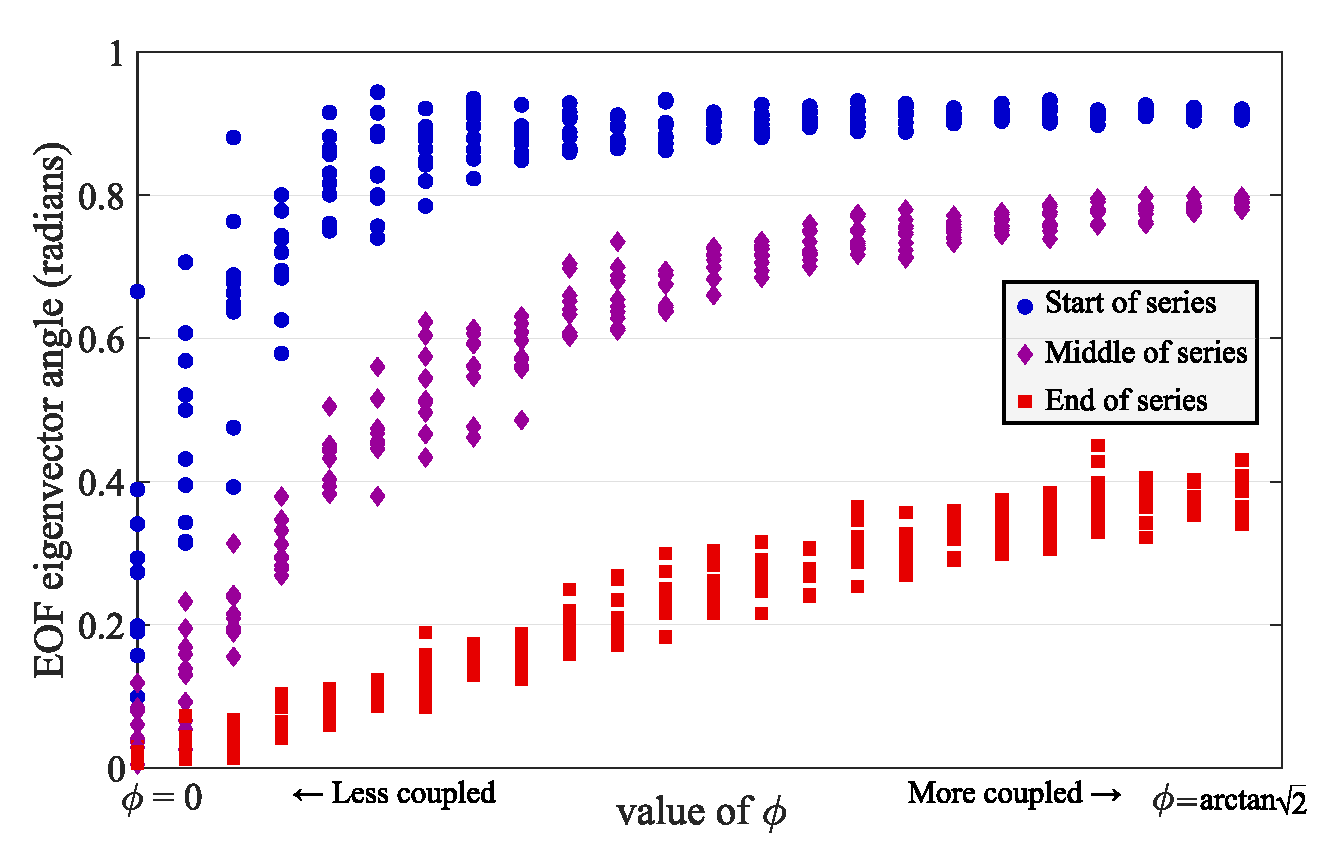
\includegraphics[width = 0.9\columnwidth]{EOFtest3D_changeS}
		\caption{The absolute value of the angle variable of the EOF eigenvector calculated in three segments of the three-dimensional series $\x_k$ (start, middle and end) using a range of $3\times 3$ matrices $S^{(\phi)}$. The series is calculated 10 times for each matrix $S^{(\phi)}$, showing the range of angles.
			\label{fig:2D:EOFtest3D_changeS}}
	\end{figure}
We note, as with the two-dimensional case, that the EOF method is more accurate at the start of the more uncoupled system series in this figure, where the segment sampled is $10^4$ points, than in figure~\ref{fig:2D:EOFtest3D_simple} where the segment size is $10^3$ points. We also note again that the EOF eigenvector at the start of the coupled system series is in the direction $(1,1,1)^\top$ with an angle $\arccos(1/\sqrt{3}) = 0.9553$ rather than $\arccos(1/\sqrt{2}) = \pi/4$ as in the two-dimensional case (from the direction $(1,1)^\top$). Again, there is very little change after about half way along the horizontal axis ($\phi>\arctan(\sqrt{2})/2$) and most of the qualitative change occurs over the first five or six values of $\phi$ used here ($\phi<0.2$). 

\subsubsection{Higher dimensions}


This same analysis is applied to higher dimensional systems where the matrix $S$ is given by the general formula
\begin{equation}
	S^{(\phi)} = 
	\frac{1}{20}\left(I_p\cos(\phi) + (J_p-I_p)\frac{\sin(\phi)}{\sqrt{p-1}} \right)\,,
\end{equation}
where $I$ is the identity matrix, $J$ is the ones matrix, and $p$ is the dimension of the system. In this way, the system changes from an uncoupled system of separate AR(1) models ($S=\sigma I$) to a coupled system ($S=\sigma J$) as $\phi$ increases from zero to $\phi_\mathrm{max}$, given by
\begin{equation}
\phi_\mathrm{max} = \arctan\left(\sqrt{p-1}\right).
\end{equation}

The results, presented similarly to the $p=3$ results in figure~\ref{fig:2D:EOFtest3D_changeS}, are shown for $p=4$ and $p=5$ in figure~\ref{fig:2D:EOFtest_changeS_4D}. We note that there is little qualitative difference as the dimension increases. 

	\begin{figure}
		\centering
		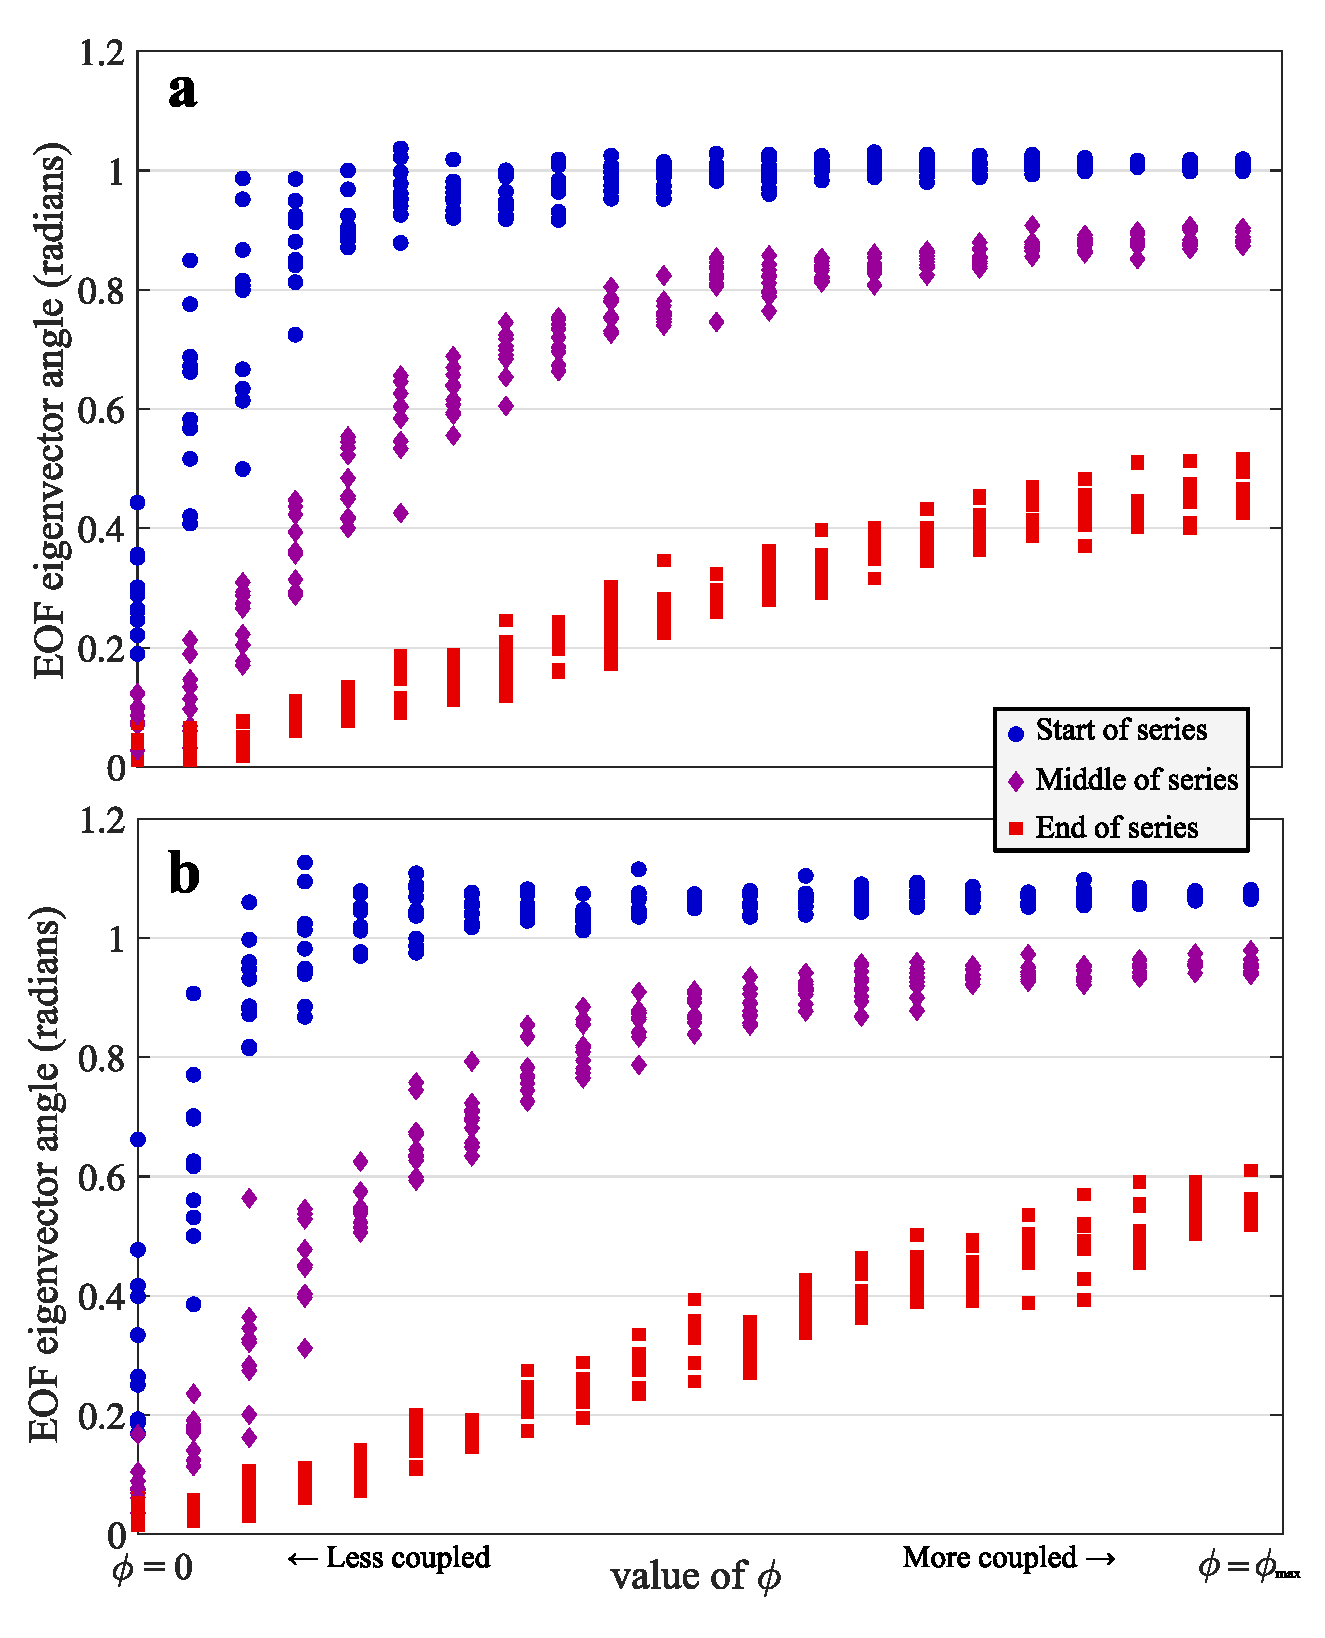
\includegraphics[width = 0.9\columnwidth]{EOFtest_changeS_4D}
		\caption{
			For four-dimensional (panel \textbf{a}) and five-dimensional (panel \textbf{b}) systems, the absolute value of the angle variable of the EOF eigenvector calculated in three segments of the series $\x_k$ (start, middle and end) using a range of $n\times n$ matrices $S^{(\phi)}$. In both cases, the series is calculated 10 times for each matrix $S^{(\phi)}$, showing the range of angles.
		\label{fig:2D:EOFtest_changeS_4D}}
	\end{figure}



\section{An alternative EOF method for dimension reduction}
\label{sec:2D:AlternativeEOF}

Although the EOF method is widely used in ecology and geosciences \citep{hasselmann1988,dommenget2001,bathiany2013p1} occasionally, even, in the process of detecting EWSs \citep{held2004}, it is not ideally suited for this purpose because it does not take into account the internal dynamics of the system. \cite{dommenget2001} note:
	\begin{quote}
		... EOF analyses have problems in identifying the dominant centres of action or the teleconnections between these centres of action in multivariate datasets. We therefore have to be very careful in interpreting the EOF modes as potential physical modes. 
	\end{quote}
\cite{hasselmann1988} proposes that the use of principal interaction patterns and principal oscillation patters (PIPs and POPs) \citep{von1995,kwasniok1996} is much better suited to applications where the evolution of a system over time is relevant, including EWS applications. The PIP technique is introduced by \cite{hasselmann1988} as an alternative to EOF analysis for reducing the dimension of a system to ``a few dominant patterns'', with the benefit that the system dynamics are modelled, similarly to an ARMA parametrisation. The use of PIPs and POPs may therefore be used to reduce the dimension of a system prior to applying one-dimensional tipping point indicators, as an alternative to EOFs. 

Besides these shortcomings, which lead one to favour PIPs and POPs as an alternative, we have noted (section~\ref{sec:2D:EOF-justification}) that it may not necessarily be the case that the EOF modes of a system will capture the largest changes in variance, which would be relevant to a variance-based EWS indicator. They are constructed so as to maximise the value of the variance. It is also not necessarily the case that the EOF modes will be relevant to an autocorrelation-based indicator. In this section we present an alternative to the EOF method where, rather than projecting the system onto a set of vectors such that the variance of the first mode is maximal (as in the typical EOF method), we do so such that the lag-1 autocorrelation is maximal. We investigate the result of using this alternative in the case of System A, described in section~\ref{sec:2D:MethodsApplied} (see equation~\ref{eqn:2D:homoclinicSystem}).
 

\subsubsection{An autocorrelation-based EOF method}

First, we consider the typical EOF method, this involves taking multiple time series and projecting onto the vector that maximises the variance. As an illustration, consider the two time series $[x_i]_{i=1}^N$ and $[y_i]_{i=1}^N$, which we assume to be mean-centred, i.e. 
\begin{equation}
\frac{1}{N}\sum_i x_i = \frac{1}{N}\sum_i y_i = 0\,,
\end{equation}
and non-dimensionalised. We then construct the matrix
	\begin{equation}
		X = \left(\begin{array}{cc}
		x_1 & y_1\\
		x_2 & y_2\\
		\vdots & \vdots\\
		x_N & y_N
		\end{array}\right),
	\end{equation}
and note that, in general, we may have any number of time series and, correspondingly, any number of columns of $X$. We now find the unit vector $\underline{u}$, and hence the time series $\mathbf{p}=[p_i]_{i=1}^N$ which is the projection of the matrix $X$ onto this vector,
	\begin{equation}
		\mathbf{p} = X\underline{u},
	\end{equation}
such that the variance of $\mathbf{p}$ is maximal given all possible unit vectors $\underline{u}$. The variance is expressed as
	\begin{equation}
		\text{Var}(\mathbf{p}) = \frac{1}{N}\mathbf{p}^2 = \frac{1}{N}(X\underline{u})^\top (X\underline{u}) = \underline{u}^\top C_0 \underline{u}\,,
	\end{equation}
where $C_0$ is the lag-zero auto-covariance matrix of $X$:
	\begin{equation}
		C_0 = \frac{1}{N}\sum_{i=1}^N \mathbf{x}_i^\top\mathbf{x}_i = \frac{1}{N}X^\top X\,.
	\end{equation}
To maximise the variance, with the constraint $||\underline{u}||=1$, we use Lagrange multipliers with the Lagrange function
	\begin{equation}
		\mathcal{L}\left(\underline{u},\lambda\right) =  \underline{u}^\top C_0 \underline{u} - \lambda\left[\left(\sum_i u_i^2\right) -1\right].
	\end{equation}
Calculating the gradient gives
	\begin{align}
		\nabla\mathcal{L} &=0\,,\\
		\frac{\partial}{\partial u_k}\left(\underline{u}^\top C_0 \underline{u}\right) - \lambda\frac{\partial}{\partial u_k}\left(\sum u_k^2\right) &= 0\,, \label{eqn:2D:maxVector_EOFreg}\\
		2C_0\underline{u} - 2\lambda\underline{u} &=0\,,
	\label{eqn:AltEOF-differentiation}
	\end{align}
since $C_0$ is symmetric, which implies $\underline{u}$ is an eigenvector of $C_0$. Say the corresponding eigenvalue is $\lambda_u$, then
	\begin{equation}
		\text{Var}(\mathbf{p}) = \underline{u}^\top C_0 \underline{u} = \underline{u}^\top \lambda_u \underline{u} = \lambda_u\, ,
	\end{equation}
because $\underline{u}^\top \underline{u}=1$. Thus to maximise $\text{Var}(\mathbf{p})$ we must choose $\underline{u}$ such that $\lambda_u$ is largest, i.e. $\underline{u}$ is the eigenvector corresponding to the largest eigenvalue of $C_0$.

Now, we may also calculate the lag-1 auto-covariance 
	\begin{equation}
		C_1 = \frac{1}{N-1}\sum_{i=2}^{N} \mathbf{x}_i^\top\mathbf{x}_{i-1} = \frac{1}{N-1}X^\top SX,
	\end{equation}
where $S$ is the matrix such that 
	\begin{equation}
		SX = \left(\begin{array}{cc}
		0\\
		\mathbf{x}_1\\
		\mathbf{x}_2\\
		\vdots\\
		\mathbf{x}_{N-1}
		\end{array}\right),
	\end{equation}
and we have the autocorrelation function 
	\begin{align}
		\begin{split}
		\text{ACF}_1(\mathbf{p}) &= \frac{\frac{1}{N-1}\sum_i p_i p_{i-1}}{\text{Var}(\mathbf{p})}\\
		&= \left(\frac{1}{N-1} (X\underline{u})^\top(SX\underline{u}) \right)\left(\frac{1}{N} (X\underline{u})^\top(X\underline{u}) \right)^{-1}\\
		&= \left( \underline{u}^\top C_1\underline{u} \right) \left(\underline{u}^\top C_0 \underline{u}\right)^{-1}.
		\end{split}
		\label{eqn:2D:maxVector_EOFalt}
	\end{align}
Now, instead of choosing a one-dimensional projection $\mathbf{p} = X\underline{u}$ such that $\text{Var}(\mathbf{p})$ is maximal, we may want to find the projection such that $\text{ACF}_1(\mathbf{p})$ is maximal. That is, we wish to find $\underline{u}_\text{max}$ such that
	\begin{align}
	\label{eqn:2D:maximumACFunitvector} 
	\begin{split}
		\text{ACF}_1(X\underline{u}_\text{max})
		 &= \max_{||\underline{u}||=1}\left[\text{ACF}_1(X\underline{u})\right]\\
		 &= \max_{||\underline{u}||=1}\left[\left( \underline{u}^\top C_1\underline{u} \right) \left(\underline{u}^\top C_0 \underline{u}\right)^{-1}\right]\,.
	\end{split}
	\end{align}
Attempting to maximise this expression in $\underline{u}$ using Lagrange multipliers, as for the simpler EOF problem (equation \ref{eqn:AltEOF-differentiation}), we obtain
	\begin{align}
	\begin{split}
		\nabla\mathcal{L} &=0\,,\\
		\frac{\partial}{\partial u_k}\frac{\left( \underline{u}^\top C_1\underline{u} \right)}{ \left(\underline{u}^\top C_0 \underline{u}\right)} &=  
		\lambda\frac{\partial}{\partial u_k}\left(\sum u_k^2\right)\,, \\
		\left(\underline{u}^\top C_0 \underline{u}\right)\frac{\partial}{\partial u_k}\left( \underline{u}^\top C_1\underline{u} \right) - \left( \underline{u}^\top C_1\underline{u} \right) \frac{\partial}{\partial u_k}\left( \underline{u}^\top C_0\underline{u} \right) &= 2\lambda \left(\underline{u}^\top C_0 \underline{u}\right)^2\underline{u}\,, \\
		\left(\underline{u}^\top C_0 \underline{u}\right)\left( C_1 + C_1^\top \right)\underline{u} - 2\left( \underline{u}^\top C_1\underline{u} \right) C_0\underline{u} &= 2\lambda \left(\underline{u}^\top C_0 \underline{u}\right)^2\underline{u}\,,
	\end{split}
	\label{eqn:AltEOF-LagrangeAttempt}
	\end{align}
which will not result in such an elegant solution and will require a tedious element-wise calculation. However, the maximisation problem can be solved using a computer, either by numerical solution of equation~\ref{eqn:AltEOF-LagrangeAttempt} or by other numerical optimisation methods applied to equation~\ref{eqn:2D:maximumACFunitvector}, once $C_0$ and $C_1$ have been calculated. A simple method to obtain a numerical solution, for problems with a low number of dimensions, is to project the time series onto many unit vectors $\underline{u}$ in a systematic way and select the $\underline{u}_\text{max}$ where the autocorrelation of $\mathbf{p}$ is largest.

\subsubsection{Application to bifurcating dynamical systems}

The method described above is applied to System A, which experiences a bifurcation when a series of stable orbits shrinks to a point and meets with a saddle node (see section~\ref{sec:2D:MethodsApplied}). The system is given by equations
	\begin{equation}
		\begin{array}{rcl}
		\dot{x} &=& y + \eta^{(x)},\\
		\dot{y} &=& \alpha - x^2 + \eta^{(y)},
		\end{array}
	\label{eqn:2D:Again-homoclinicSystem}
	\end{equation}
where $\eta^{(x)}$, $\eta^{(y)}$ are white noise terms. The system is integrated and sampled with a time step of $\Delta t = 0.5$ to produce a time series of 200 points (in each variable). The ACF-based EOF method is then applied to the two variables to reduce the dimension, yielding a one dimensional time series. To do this, the maximisation problem in equation~\ref{eqn:2D:maximumACFunitvector} is solved element-wise using Matlab's standard \texttt{fmincon} interior-point optimisation algorithm \citep{dennis1996numerical, byrd1999interior, byrd2000trust} to find $\underline{u}_\text{max}$, and the one-dimension projection $X\underline{u}_\text{max}$ is calculated, where $X$ is the mean-centred data matrix.

\begin{figure}
	\centering
	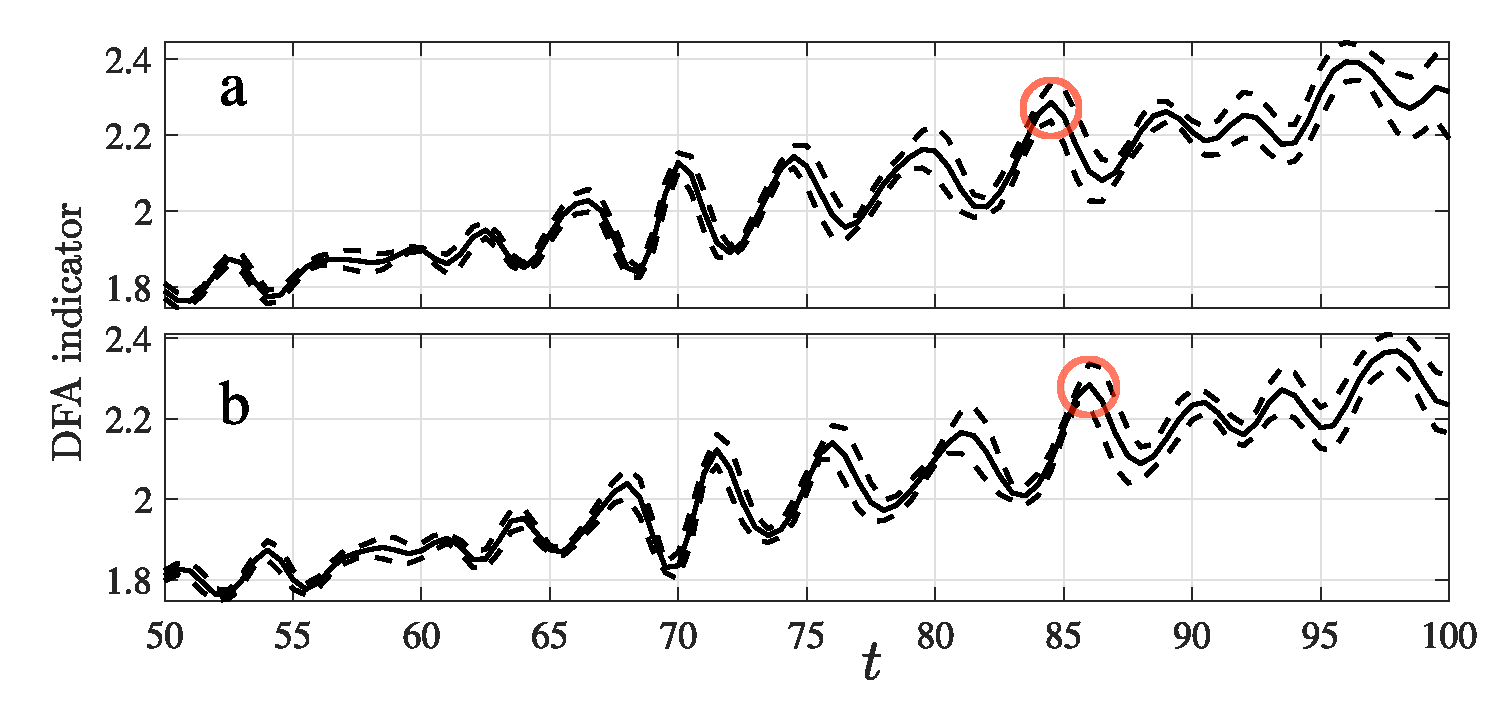
\includegraphics[width = 0.9\columnwidth]{AltEOFDFA_homoclinic}
	\caption{DFA indicator with a window of 100 points calculated for the one-dimensional time series obtained using the variance-based EOF technique (panel \textbf{a}) and the autocorrelation-based EOF technique (panel \textbf{b}) applied to the system described by equation~\ref{eqn:2D:Again-homoclinicSystem}, which experiences a bifurcation at $t=100$. In each panel the plot shows the mean over ten realisations of the dynamical system, with error bounds of one standard deviation. One example of a common feature is circled in red.
		\label{fig:2D:AltEOFDFA_homoclinic}}
\end{figure}

Having obtained the one-dimensional time series $X\underline{u}_\text{max}$ via this autocorrelation-based EOF technique, the DFA indicator is calculated with a window size of 100 points: figure~\ref{fig:2D:AltEOFDFA_homoclinic}b shows the result and, for comparison, the same process is also performed using the regular variance-based EOF technique (panel~\textbf{a}).  We see that there is little difference in the DFA indicator whichever EOF technique is used, the same features appear in both signals. However, the features appear earlier when the regular, variance-based EOF technique is used (panel~\textbf{a}). An example of a shared feature (a peak in the oscillating DFA indicator signal) is circled in red in figure~\ref{fig:2D:AltEOFDFA_homoclinic}: this feature occurs before $t=85$ in panel~\textbf{a} but slightly after $t=85$ in panel~\textbf{b}. This is not an artefact of the alternative EOF technique producing a lagged time series due to the lag in the autocorrelation, since only the lag-1 ACF is used and a single time step is of length $\Delta t=0.5$, whereas the apparent shift in the features of the DFA indicator signal is $\approx 1.5$. Rather, this is simply due to the different projection used to obtain the one-dimensional time series to which the DFA indicator is applied. 

To investigate the alternative EOF technique further, we also apply it to the other two-variable dynamical systems described in section~\ref{sec:2D:MethodsApplied}: the system experiencing a Hopf bifurcation (equation~\ref{eqn:2D:HopfSystem_noise}), to which we refer as "system B"; and the Van der Pol oscillator (equation~\ref{eqn:2D:VDPSystemCoupled}), or "system C". The system described in equation~\ref{eqn:2D:Again-homoclinicSystem} is referred to as "system A". Each of the three systems is integrated 100 times and both EOF techniques are applied to each resulting two-variable time series. In each case we record the eigenvector onto which the system is projected to obtain the one-dimensional time series. A multivariate time series has, for this purpose, two vectors $v_V, v_A$, characterised by their angles $\theta_V, \theta_A\in (-\pi,\pi]$, associated with it, and onto which we may chose to project it. The vector $v_V$ is the unit vector which maximises the variance, as the vector $\underline{u}$ in equation~\ref{eqn:2D:maxVector_EOFreg}, used in the regular variance-based EOF technique. The vector $v_A$ is the unit vector which maximises the autocorrelation, used in the alternative autocorrelation-based EOF technique. These vectors, for the three dynamical systems, are represented graphically on the half-circle in figure~\ref{fig:2D:EOFeigenvectors_comparison}. We see that in all three systems there is little variability in the variance-maximising vector (displayed in blue) but the autocorrelation-maximising vector is more sensitive to differences between different realisations of the system. This effect is visible, in particular, in System A, which is the subject of the study with the DFA indicator in figure~\ref{fig:2D:AltEOFDFA_homoclinic}. For each realisation of each system the angle difference $|\theta_V-\theta_A|$ is calculated and the mean is found to be 0.510 ($29.2^\text{o}$) in system A; 0.184 ($10.6^\text{o}$) in system B; and 0.162 ($9.30^\text{o}$) in system C. That is, in all three systems, the vector $v_A$ is closer to $v_V$ than the perpendicular. Particularly in systems B and C there will be little observable difference between the two projected time series. 


\begin{figure}
	\centering
	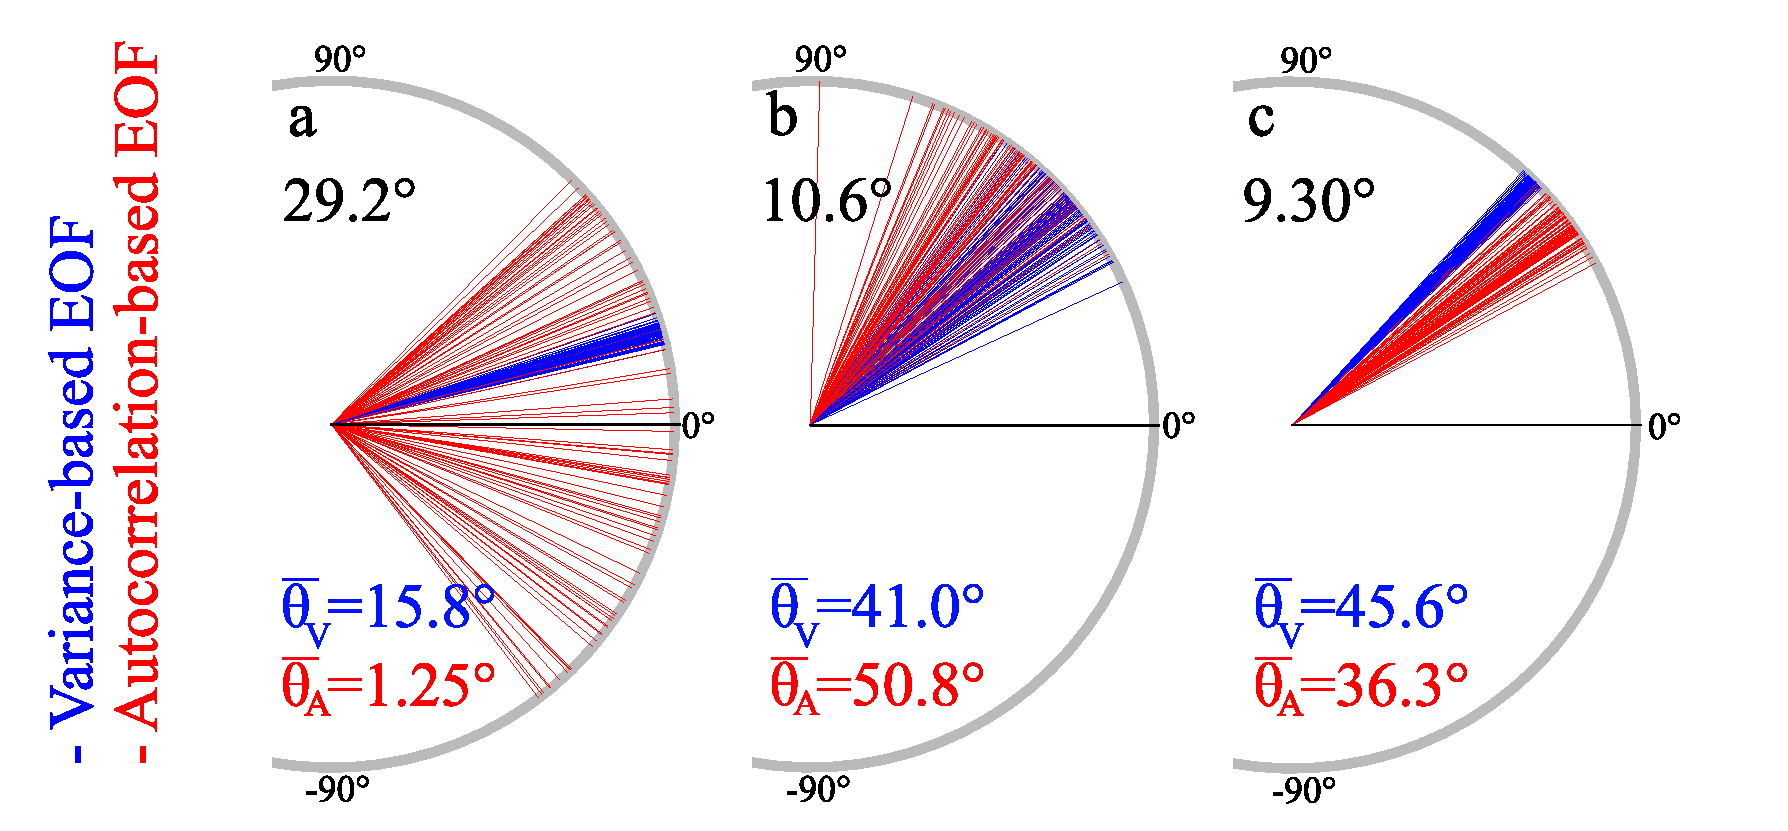
\includegraphics[width = 0.9\columnwidth]{EOFeigenvectors_comparison}
	\caption{Eigenvectors on the unit half-circle used to obtain the projection involved in the EOF technique (blue) and the alternative autocorrelation-based EOF technique (red) applied to 100 realisations of each dynamical system. Panel~\textbf{a}: system A (equation~\ref{eqn:2D:Again-homoclinicSystem}). Panel~\textbf{b}: system B (equation~\ref{eqn:2D:HopfSystem_noise}). Panel~\textbf{c}: system C (equation~\ref{eqn:2D:VDPSystemCoupled}). The mean difference (in degrees) in the angles, $\overline{|\theta_V-\theta_A|}$, is displayed in black font beneath the identifying panel letter. The mean angles $\overline{\theta_V}$ and $\overline{\theta_A}$ are displayed in their respective colours.
		\label{fig:2D:EOFeigenvectors_comparison}}
\end{figure}



\section{EWS in spatial data}
\label{sec:2D:ExtensionToGridded}

Besides techniques which allow one to detect or predict a tipping point in a multivariate system, we are also interested in dynamical systems evaluated over a data field. In a scenario where one has, for example, many time series associated with locations over a 2D field, one may reduce the dimension of the system using the EOF method to condense all of the available information. This can be refined if a specific region of interest is identified in advance: \citet{ludescher2013,ludescher2014} calculate the cross-covariance of a variable, at a specific time slice, between points inside the El Ni\~{n}o basin and points outside. In contrast, simply using the EOF method to reduce the dimension of such a system will not give specific spatial information such as the location of the tipping point or the direction of its progression in the case that a tipping at one location precipitates a tipping at other locations. However, one may also wish to use the spatial locations of the data, for example, to predict the location of the disturbance (a "hotspot") which is causing the tipping point: that is, locations where critical slowing down, and therefore loss of stability, is most apparent. \citet{bathiany2013p1} present a method to detect these hotspots: the method involves partitioning the locations ("elements") and, within each partition, discovering which elements contribute the most to the autocorrelation. This is done by combining the elements in different permutations, projecting onto the EOFs, and calculating the lag-1 autocorrelation of the resulting signal. Elements in each part are removed according to system-specific selection criteria and the remaining elements are re-partitioned. The process is repeated until only one partition remains, which is the slowing down hotspot where susceptibility to perturbations is large. The method is applied successfully to a highly idealised model of a vegetation cover. A similar method, also in the context of vegetation and aridity, is used by \citet{kefi2014early} who calculate the spatial correlation of the points across a two-dimensional field — the spatial variance and spatial frequency (where emerging spatially-repeating patterns are a symptom of the tipping) are also considered.

In this section we present a method to visualise the behaviour of the one-dimensional tipping point indicators introduced in chapter~\ref{chap:1D} evaluated at multiple locations, at a specific time slice, thus allowing one to observe locations, or hotspots, where a tipping point is likely to occur. 

\subsubsection{A 2D visualisation of indicator behaviour}

In figure \ref{fig:tikz-approachingfront} we illustrate an example of a propagating front over a 2D field. The time series $z_{xy}(t)$ is evaluated at each point $(x,y)$ on the field, and a tipping point occurs at the front (double line) which propagates from top-right to bottom-left. If we take the time series at points {\bf A} and {\bf B} and perform an EWS analysis, for example calculating the ACF1 indicator in a sliding window, we expect that the EWS will be stronger at point {\bf B} than at point {\bf A} because the tipping is closer (in time) to {\bf B}. Given some knowledge of the nature of the system one could conclude that the front is approaching from the right (from the positive $x$ direction) and, performing the analysis for more points in a grid over the field, one could determine more precisely the shape of the front and its direction. 

It will be difficult to visualise an ACF1 indicator series at every point on the grid (assuming the grid is larger than 3-by-3) in order to determine at which points the EWS is strongest. It is therefore useful to measure the increase in the indicator value at a specified point in time and to create a contour plot of this value over the grid.

\begin{figure}
	\centering
	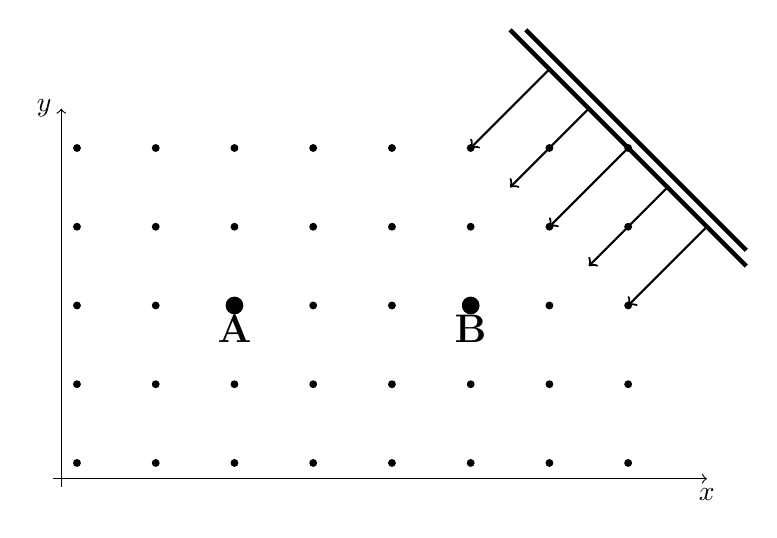
\begin{tikzpicture}
	\draw[->] (-2.3,-2.2) -- (6,-2.2) node[below] {$x$};
	\draw[->] (-2.2,-2.3) -- (-2.2,2.5) node[left] {$y$};
	
	\foreach \x in {-2,-1,...,5} {
		\foreach \y in {-2,-1,...,2} {
			\fill[color=black] (\x,\y) circle (0.05);
		}
	}
	
	\filldraw (0,0) circle (3pt) node[below] {\Large \bf A};
	\filldraw (3,0) circle (3pt) node[below] {\Large \bf B};
	
	\draw[-, ultra thick] (3.5, 3.5) -- (6.5,0.5);
	\draw[-, ultra thick] (3.7, 3.5) -- (6.5,0.7);
	\draw[->, thick] (4,3) -- (3,2);
	\draw[->, thick] (4.5,2.5) -- (3.5,1.5);
	\draw[->, thick] (5,2) -- (4,1);
	\draw[->, thick] (5.5,1.5) -- (4.5,0.5);
	\draw[->, thick] (6,1) -- (5,0);
	\end{tikzpicture}
	\caption{Propagating front. The time series $z_{xy}(t)$ is evaluated at each point on the field, and a tipping point occurs at the front (double line) which propagates from top-right to bottom-left. We expect that an EWS of the tipping point will be stronger at point {\bf B} than at point {\bf A} because the tipping is closer (in time) to {\bf B}.}
	\label{fig:tikz-approachingfront}
\end{figure}

As an example, we consider a system with a pitchfork bifurcation, which was used as an example in section \ref{sec:1D:indicatorComparison}. In this example, many similar dynamical systems are defined over the discrete $xy$ plane $\mathbb{Z}^2$, by the equation 
	\begin{equation}
		\frac{dz_{xy}}{dt} = -\frac{\partial}{\partial z_{xy}}\left(z_{xy}^4+\frac{\mu-x-y}{10}z_{xy}^2\right)+\sigma\eta_{xy},
	\label{eqn:propagatingPitchfork}
	\end{equation}
where the $\eta_{xy}$ are independently distributed Gaussian noise series. The line $y=-x+\mu$ defines the front: if $x+y<\mu$ the $z^2$ coefficient is positive and the system $z_{xy}(t)$ has a double-well generalised potential function; if $x+y\geq\mu$ then the system has a single-well potential. 

We create a 10-by-10 grid and integrate equation \ref{eqn:propagatingPitchfork} at each point $(x,y)$ from $t=0$ to $t=1000$ with time step $\Delta t = 0.05$. Parameter $\mu$ is made to decrease linearly at each time step so that at $t=0$, $\mu = 20$ and at $t=1000$, $\mu=10$. The series is sampled, after the integration, at intervals of one time unit to give a series of length 1000 points. For each time series $z_{xy}$, the ACF1 indicator is calculated in a sliding window of 100 points. In order to determine the location of the moving front at time $t$, one must determine whether the ACF1 indicator is increasing at each point $(x,y)$. We use the Mann-Kendall coefficient given by the equation
	\begin{equation}
		\label{eqn:2D:KendallCoef} 
		c(X) = \frac{2}{N(N-1)}\sum_{i=1}^{N-1}\sum_{j=i+1}^{N}\text{sign}(X_j-X_i),
	\end{equation}
for a time series $X$. This coefficient $c$ is calculated for each indicator series in the range $[t-100, t]$, thus showing whether the indicator series is increasing (positive coefficient) or decreasing (negative) in the 100-point window prior to time $t$. Figure~\ref{fig:2D:PitchforkContour-N10} shows the result when $t=1000$, that is, the time when $\mu=10$ and the pitchfork bifurcation is occurring in systems $z_{xy}$ on the line $x+y=10$. To the top-right of this line, the bifurcation has already occurred and the lag-1 ACF is decreasing (negative Mann-Kendall coefficient). To the bottom-left of this line, the systems have not yet bifurcated and the ACF1 indicator is increasing (positive Mann-Kendall coefficient) as an EWS of the approaching tipping point. As demonstrated in the simple application of the ACF1 indicator to the pitchfork bifurcating system in section \ref{sec:1D:indicatorComparison}, there is some variability in the indicator series and we cannot expect a completely smooth gradient to appear in the contour plot. However, the figure \ref{fig:2D:PitchforkContour-N10} does accurately represent the existence of a front. We note that a clear line between positive and negative appears to exist along the line $x+y =11$, because of the lag effect caused by the window size of 100 points used in the calculation of both the ACF1 indicator and the Mann-Kendall coefficient. This effect can be taken into account to conclude that the bifurcation is actually occurring some way in before the front apparent in the figure. The speed at which the front is advancing can be ascertained by taking snapshots of the system at intervals, that is, using a varying values of $t$ when calculating the Mann-Kendall coefficient in the preparation of the contour plot.
\begin{figure}
	\centering
	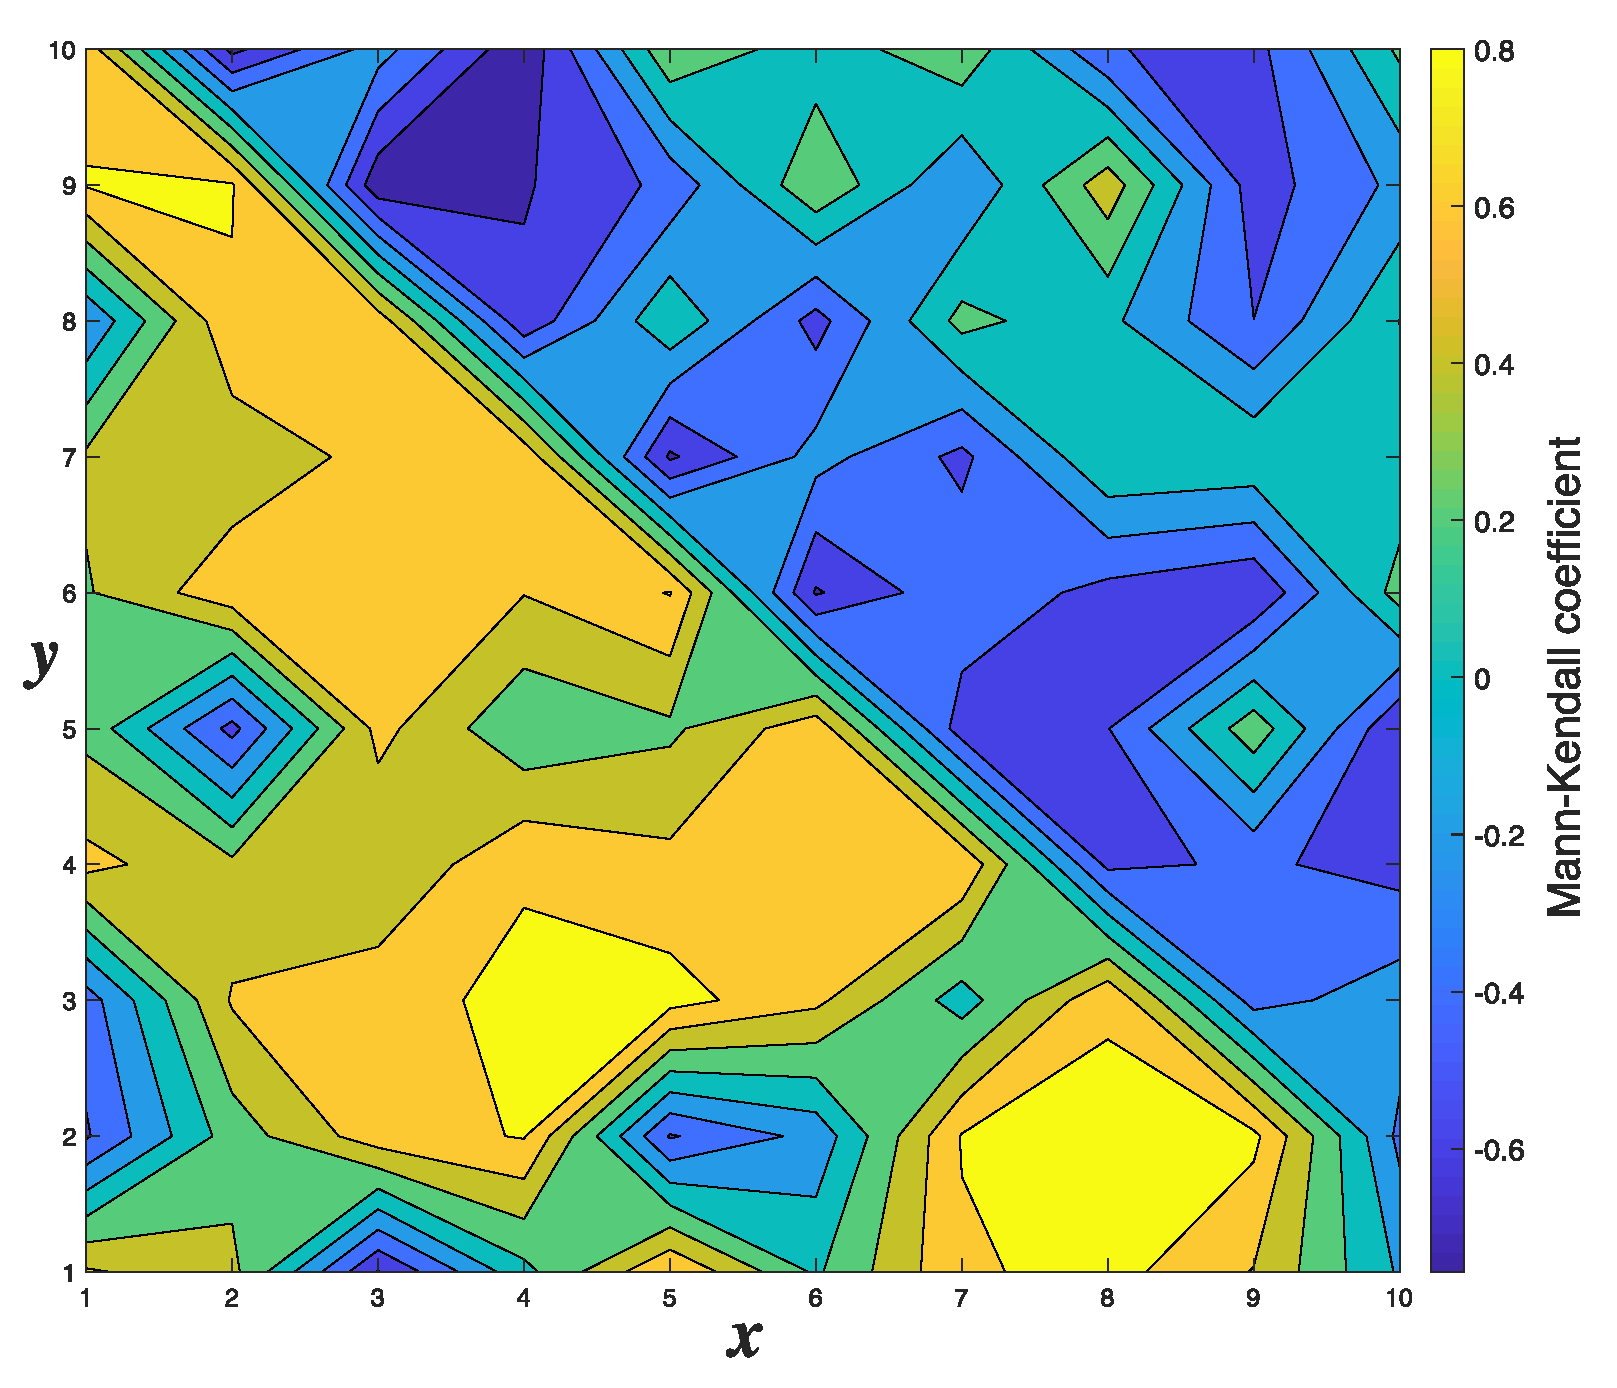
\includegraphics[width=0.9\textwidth]{PitchforkContour_N10}
	\caption{A 2D bifurcation caused by an approaching front. At each point $(x,y)$ a system is described by equation \ref{eqn:propagatingPitchfork} where the value of $\mu$ is decreasing. The figure shows the Mann-Kendall coefficient of the ACF1 indicator of the series when $\mu=10$, when the bifurcation is occurring at points on the line $y+x=10$. To the top-right of this line, the bifurcation has already occurred and the lag-1 ACF is decreasing (negative Mann-Kendall coefficient). To the bottom-left of this line, the systems have not yet bifurcated and the ACF1 indicator is increasing (positive Mann-Kendall coefficient) as an EWS of the tipping point.}
	\label{fig:2D:PitchforkContour-N10}
\end{figure}

If the experiment is repeated several times and the Mann-Kendall coefficient is calculated for the mean over all ACF1 indicator series at each point, the variability in the indicator will be smoothed and the line representing the front will be clearer. This may be necessary for systems where the indicator series contain greater variability, but impractical for applications where the experiment occurs only once.


\section{Discussion}
\label{sec:2D:discussion}

In this chapter we have presented techniques for detecting early warning signals in time series of more than one variable. The first technique, introduced by \citet{williamson2015}, reconstructs the eigenvalues of the system's Jacobian matrix using the relationship to the autocorrelation matrix. These eigenvalues are then used as indicators of a tipping point based on assumptions about the nature of the tipping. For example, a Hopf bifurcation in a two-variable system occurs when the Jacobian eigenvalues cross the imaginary axis, so calculating the behaviour of the imaginary part over time will provide a useful indicator which predicts a bifurcation as it approaches zero. The other technique presented uses EOFs to reduce the dimension of the system, before applying a familiar one-dimensional indicator to the resulting one-dimensional time series. We have applied both of these techniques to time series data from three known two-variable dynamical systems. In all cases the DFA indicator applied to the first EOF series provided a clear EWS in the mean. The ACF and PS indicators applied to the first EOF series did not give such a clear signal. The reconstructed Jacobian eigenvalues did provide an EWS in some cases, but it is necessary to know which eigenvalue to use.

We noted that the use of EOFs to reduce the dimension of a system, in an EWS context, assumes that the relevant signal will not be lost in the process. The EOF method projects a time series in such a way as to maximise the variance, which may not maximise the increase in the relevant tipping point indicator. We calculated the EOF scores analytically of a general linear dynamical system. We found that, except in contrived cases with very large variance in one variable, the EOF projection vector is similar to the direction in which the system diverges at a tipping point. We also devised an alternative EOF method which maximises the lag-1 autocorrelation of the projection rather than the variance. When applied to three dynamical systems we found that the projection vector was similar to that for the regular, variance-based, EOF method, but there was greater variability. 

In addition to this work, which concentrates on time series in several variables, with examples of two-variable systems, we have also studied dynamical systems defined over a discrete two-dimensional field. This type of data are particularly common in meteorology where data is collected at discrete locations over a geographic area (including the entire globe). We have proposed a simple method which may be used to visualise tipping point indicators over a field, and have applied this to an example based on a simple pitchfork bifurcation for which a reliable EWS can be obtained. This is a method to aid the visualisation of the tipping point indicator and it works as expected.

\subsubsection{Future work}

In the chapter we have used three dynamical systems as examples. It is always possible to apply the techniques presented here to more systems with different types of tipping. This work has been done with an aim of demonstrating the validity of using various techniques, rather than with a view to studying early warning signals in a comprehensive collection of dynamical systems. Indeed, when meteorological data is presented the type of tipping is often unknown: that is, it is not known whether or not the tipping is caused by, for example, a Hopf bifurcation in the underlying system. It is therefore useful to have a variety of techniques available that could be compared to infer the possible nature of the critical transition.

When calculating the EOF eigenvectors analytically for the general linear system, we did not calculate an error term by considering the variance in the system, we have only considered the mean. This does not appear to be possible without making further simplifications to the equations, but it may be possible to provide an estimate in future work.

It would be particularly interesting to use a general, simple system which is relevant to a meteorological event. In the next chapter, a specific model of a tropical cyclone is presented as a further test of the technique.


